\documentclass[prd, nofootinbib, floatfix, 11pt,tightenlines,times]{article}

% latex W13report.tex; bibtex W13report; latex W13report; latex W13report; dvips W13report; ps2pdf W13report.ps ; gv W13report.pdf

\usepackage[paperwidth=8.5in,paperheight=11in,centering,margin=1in]{geometry}
\usepackage{amsmath}
\usepackage{amsbsy}
\usepackage{natbib}
\usepackage{rotating}
\input epsf
\usepackage{amsmath}
\usepackage{caption}
\usepackage{wasysym}
\usepackage{subfig}
\usepackage{graphicx}
\usepackage{epsfig}
\usepackage{color}
%\usepackage{ulem}
%\usepackage{epstopdf}
\usepackage[toc,page]{appendix}

\renewcommand{\thefootnote}{\fnsymbol{footnote}}

%\renewcommand{\baselinestretch}{0.98}
\usepackage{epsfig}
\usepackage{titletoc}

% HOW TO SET UP AN 8.5 x 11:
% http://www.pages.drexel.edu/~pyo22/students/latexRelated/latexTutorial.html
\topmargin -1.5cm        % read Lamport p.163
\oddsidemargin -0.04cm   % read Lamport p.163
\evensidemargin -0.04cm  % same as oddsidemargin but for left-hand pages
\textwidth 16.59cm
\textheight 21.94cm 
\parskip 7.2pt           % sets spacing between paragraphs
\parindent 0pt		     % sets leading space for paragraphs

\def\aap{{\it Astr.~Ap.}}     %Astronomy & Astrophysics%
\def\aaps{{\it A\&AS}}
\def\apj{{\it ApJ}}

\author{Andrew Becker, Simon Krughoff, Andrew Connolly, Russell Owen\vspace{-2ex}}
\title{Report on Late Winter2013 Production: Image Differencing\vspace{-2ex}}
\date{\vspace{-2ex}\today}

\begin{document}

\maketitle
\vspace{-2ex}
We provide here a technical report on the LSST Data Management
late--Winter 2013 production runs.  This production focused on the
evaluation of LSST DM image differencing code, in particular on
evaluating the rate of false detections the pipeline generates.  As
inputs, we used a suite of simulated images generated in idealized
conditions and containing no intrinsic variability.  Thus {\it any}
sources detected in these image differences are ``false positives''.

We investigated two distinct operational modes of the pipeline.  The
first pre--filters the science image with its own PSF, yielding a
point--source maximum likelihood image.  The template is then
PSF--matched to this image, subtracted from it, and detection and
measurement happen directly on this difference.  The second mode
matches the template image to the science image, creates their
difference, post--filters the difference with the science image PSF,
and then runs detection on this maximum likelihood image.  Measurement
happens on the detected footprints, but in the difference image.  We
also investigated the complexity of the basis functions used to model
the PSF--matching kernel, and the degree to which this kernel varies
across the images.  We generated several goodness of fit statistics
for a control sample of sources that were {\it not} used in the kernel
fit, in order to assess the interpolation ability of the matching
kernel.

We compared the measured numbers of false detections to the number we
expect due to random fluctuations in a background Gaussian field.  The
latter is a function of both seeing in the images, and of the
detection threshold used.  At the fiducial detection threshold of
5--sigma, the number of expected false positives per LSST sensor is of
order {\bf XX}, and we measure of order {\bf YY}, indicating that we
are able to achieve the systematic floor in false detection rate.  We
examined our measured false detection rate as a function of detection
threshold and find that it roughly scales as expected.  In order for
there to be less than 1 expected false detection per sensor, we must
operate at a detection threshold of {\bf X.X} sigma.

We found a severe dependence of the false positive rate on our
understanding of the variance; even a 1\% misestimate of the noise may
increase or decrease the false positive rate by a factor of {\bf XX}
at 5--sigma.  Prefiltering is preferred in this regard, as our
variance planes are shown to track the variance to higher fidelity at
the detection stage.  We find that over/undersubtraction of the image
background leads to a bias in the positive to negative false detection
ratio, but not on the overall numbers of detections.  Prefiltering
also prevents, in many cases, a deconvolution of the template image
when the science image has better seeing, which is a clear advantage
of the technique.

We outline several additional steps we will pursue on the Summer 2013
timescale, including operating on images with more astrophysical and
atmospheric complexity, improving measurement on PSF--filtered
sources, adopting Gaussian processes for modeling of the spatial
kernel, and using statistics calculated during the image subtraction
to tune the algorithm ``on the fly'' (i.e. predict the numbers of
false positives it will generate).



\clearpage
\tableofcontents
\clearpage

\section{Production Scope and Goals}

The focus of this production was to optimize and quantify the false
detection rate in the PSF--matched subtraction of a science image and
a reference image (referred to as the template image below).  We used
simulated images generated using ideal conditions, and with no
intrinsic variability in the sources.  The metric we optimized is the
number of false detections that are detected and measured on the image
difference.  As the input were simulated with no variability, any
detections found in the difference images are ``false positives''.  We
calculated several additional quality metrics during the image
subtraction process, and correlated them with the number of false
detections, as a means to predict the number of false detections we
may expect downstream from the image subtraction.  Once we found an
optimum configuration, we perturbed the solution along multiple
dimensions to understand how the false detection rate responded.  

\subsection{Algorithm and Background}

We outline the image subtraction process below.  We assume that science
image $S(x,y)$ can be modeled as a convolution of the template image
$T(x,y)$ by a PSF--matching kernel $K(u,v,x,y)$.  The images will have
different point spread functions (PSFs), which are the time--averaged
transfer functions of a point source through the Earth's atmosphere,
telescope optics, and into the silicon of the detector before being
read out.  The essence of image subtraction is to match the PSFs of
these two images so that they may be subtracted pixel by pixel.  We
further assume that the PSF--matching kernel may be decomposed using a
set of basis functions $K(u,v) = \sum_i a_i K_i(u,v)$, where the
coefficients in front of each basis are determined through:
%
\begin{eqnarray}
C_i & \equiv & (K_i \otimes T) \\ \nonumber
b_{i}  & = & \sum_{x,y} {{C_i(x,y) S(x,y)}\over{\sigma^2(x,y)}}   \nonumber \\ 
M_{ij} & = & \sum_{x,y} {{C_i(x,y) C_j(x,y)}\over{\sigma^2(x,y)}}  \nonumber \\ 
a_{i}  & = & M^{-1}_{ij} b_{j} \nonumber 
\label{eq-soln}
\end{eqnarray}
where $\sigma^2(x,y)$ is the per--pixel variance stored in the {\tt
  variance} plane of each LSST {\tt exposure}.  To generate a
spatially varying model for the kernel, we assume that the relative
weights of the basis functions $a_i$ themselves vary spatially,
i.e. $K(u,v,x,y) = \sum_i a_i(x,y) K_i(u,v)$.  We also assume that
there is a differential background between the two images $b(x,y)$
that may be fit for using a low--order Chebyshev polynomial.  The
image difference is then calculated through $D(x,y) = S(x,y) - T(x,y)
\otimes K(u,v,x,y) - b(x,y)$.

The basis functions themselves $K_i(u,v)$ are a degree of freedom in
this problem.  The original implementations \citep{Alard98,Alard00}
used a set of 3 Gaussians (represented by our {\tt Config} variable
nGauss), each with a different sigma (sigGauss), and each modified by
a Laguerre polynomial to a given order (degGauss).  Subsequent studies
\citep[e.g.][]{2007AN....328...16I} have suggested that a constant
ratio be maintained between the different Gaussian widths, such that
$\sigma_{i+1} = \beta \times \sigma_{i}$.  We use the value $\beta =
2.0$ for this production.  We set the overall scale for sigma by
noting that, under the assumption that the PSFs of the images are
Gaussian ($\sigma_S$ for the science image and $\sigma_T$ for the
template image), the sigma of the matching kernel should be simply
$\sigma_K^2 = \sigma_S^2 - \sigma_T^2$.  We use this width for the
central Gaussian in the basis sequences where we use more than one
Gaussian, or the sole Gaussian in the sequences when we use only one.

Detection on the difference image occurs through correlation of
$D(x,y)$ with the science image's PSF, yielding optimally filtered
detection image $D'(x,y) = D(x,y) \circ PSF_S(x,y,u,v)$ where $\circ$
denotes correlation.  The values of the pixels in $D'(x,y)$ provide a
maximum likelihood estimate of there being a point source at that
position.  Detection occurs by simply finding pixels that are more
than N sigma above the variance.  

In this production, we investigated two orders of operations for the
optimal filtering by the PSF.  In the first method, called
prefiltering, we PSF--match the template image to a pre--filtered
science image:
\begin{eqnarray}
D_{Pre}(x,y) & = & S(x,y) \circ PSF_S(x,y,u,v) - T(x,y) \otimes K(u,v,x,y) \nonumber \\ 
D'_{Pre}(x,y) & = & D_{Pre}(x,y). \nonumber 
\end{eqnarray}
By pre--smoothing the image that we are matching the template to --
$S(x,y) \circ PSF_S(x,y,u,v)$ -- we more frequently avoid the case of
PSF--matching {\it deconvolution}, where the FWHM of $T$ is broader
than $S$.  This pre--filtering increases $\sigma_S$ by $\sqrt{2}$.
The PSF matching kernels will need to be correspondingly larger to
account for the larger effective PSFs.  We are able to run detection
directly on this image.

In the second, which is the classical postfiltering implementation of
the technique, we create a difference image that is then
post--filtered with the PSF for detection:
\begin{eqnarray}
D_{Post}(x,y) & = & S(x,y) - T(x,y) \otimes K(u,v,x,y) \nonumber \\ 
D'_{Post}(x,y) & = & D_{Post}(x,y) \circ PSF_S(x,y,u,v).  \nonumber 
\end{eqnarray}

%One complication is that measurement on $D'_{Pre}$ is necessarily
%different than on $D'_{Post}$.

\section{Input Data}

Specialized simulations were developed with constrained astrophysical
complexity for the initial test data. The purpose of these images was
to define a baseline for how well image subtraction would perform in
the absence of chromatic effects (e.g.\ differential chromatic
refractions), and perturbations in the optical system. To accomplish
this the data comprised $i$-band simulations of a random distribution
of stars with a density of $\sim 1000$ stars per CCD and with an
equivalent $r$-band magnitude range ($19<r<21$). All stars in this
sample had identical spectral energy distributions
(km50\_5000.fits\_g20\_5140.gz), and, for all sources, variability,
proper motion, and parallax were set to zero. All simulations were
made at the zenith.

Nine sensors of the central raft were simulated, for a total of 27
difference images per configuration to use in our comparative
analysis.  Each simulation run was generated using the following
configurations:
\begin{itemize}
\item Visit 6866600: A pair of 300s exposure template images with
  an atmospheric seeing value of 0.88 arcsec.
\item Visit 6866601: A pair of 15s exposure exposures with 0.6
 arcsec atmospheric seeing.
\item Visit 6866602: A pair of 15s exposure exposures with 0.88
 arcsec atmospheric seeing.
\item Visit 6866603: A pair of 15s exposure exposures with 1.2
 arcsec atmospheric seeing.
\end{itemize}

For each configuration, v3.2.5 of the LSST phosim package was used to
generate the data. The sky background was dark and set to produce
$\sim$150 counts per pixel, with airglow variations set to
zero. Telescope and camera perturbations, tracking errors, field
rotation, and saturation and blooming effects were all disabled. To
enable the use of eimages directly within the analysis (i.e.\ to
remove the need for the construction of a full CCD from the amplifier
images, calibration of the simulated data, and the generation of
photometric zero points) the pixel quantum efficiency variations were
set to zero, cloud screens were turned off and no cosmic rays were
generated.  The phosim commands file for the generation of the
simulated data listed in Appendix~\ref{sec-phosim}.  Reference
catalogs and astrometry.net indices were constructed from the input
catalogs.  A secondary set of simulation images was generated for the
extended analysis.  These data are described in
Appendix~\ref{sec-phosimextend}.

\section{Work Performed}

Major tasks that were completed in the run--up to production include:
implementing prefiltering for image subtraction (ticket \#2551);
implementing source selection for image subtraction (\#2554, \#2596);
implementing measurement for difference image source ({\tt DiaSource})
characterization (\#2595); implementing RegisterTask for
image--to--image registration (\#2562, \#2650); defining and
implementing metrics for testing ip\_diffim (\#2636); designing a tool
to scrape metadata from data repositories (\#2640); and implementing
flux measurement for PSF--filtered sources (\#2754).

Below we describe in detail the overall pipeline that was established
as the results of these tasks.  We follow with in--depth analysis of
implemented algorithms that are central to this production.

\subsection{Pipeline Implementation}

At the beginning of the pipeline, we have as an input the science
image $S(x,y)$ as a {\tt calexp} instance.  The bounding box of the
science image, in celestial coordinates, is ideally used to query the
coadd repository to return the coadd patches that overlap the image.
However, because of difficulties in fitting absolute astrometry to the
images (Section~\ref{subsec-astrom}), we instead took the approach of
directly using the {\tt calexp} of the deep visit (v6866600) as the
reference visit (as opposed to taking this deep {\tt calexp} and
turning it into a coadd).

Next, we used the DiaCatalogSourceSelector to query the ImSim
reference catalog for appropriate sources to use for PSF matching.
This selector allows the user to specify the brightness and color
range of the objects, toggle star or galaxy selection, and to include
variable objects or not.  We selected a fraction (1/5) of these
objects to serve as a control sample, in order to assess the
effectiveness of $K(u,v,x,y)$ to subtract objects that were {\it not}
used in the least squares fit.

The reference and science {\tt calexps} were then astrometrically
registered to each other, with the resampling operations happening on
the reference visit as it has the larger signal--to--noise (S/N).
Object--to--object matching, done using the source list above
cross--matched with a source list extracted from the coadd, was used
to provide a relative astrometric transformation between the two
images.  RegisterTask was used to do the resampling.  The resulting
warped reference image was what we use as the template image $T(x,y)$.
The residuals of the object--to--object match were persisted as part
of the debugging infrastructure.  We assumed that the background
subtraction on the input {\tt calexps} removed the high order features
in the backgrounds; therefore we simultaneously fit for a 1st--order
spatially varying differential background $b(x,y)$ along with the
kernel coefficients.

Images $S(x,y)$ (optionally pre-filtered with $PSF_S(x,y,u,v)$) and
$T(x,y)$ were sent to ImagePsfMatchTask, whose purpose is to fit for
$K(u,v,x,y)$ and to produce $D(x,y)$.  The first step is to use the
PSF Gaussian sigmas to define the {\it sizes} of the Gaussians shapes
in $K_i(u,v)$.  As mentioned above, the main width was chosen to be
$\sqrt{\sigma_S^2 - \sigma_T^2}$.  We investigated variations on the
configuration where we used one Gaussian with the above width, and
where we used three Gaussians, the central of which has this width and
the others are a factor of $\beta = 2.0$ smaller and larger.  We
modified each of the Gaussians by a set of Laguerre polynomials of a
given order.  The smallest Gaussian was modified to the specified
order, with the others modified by order//2.  Figure~\ref{basis}
provides an example basis set with this configuration.  The total
number of shapes in each basis were: $\sum_i^{\rm nGauss} ({\rm
  degGauss}_i+1)\times({\rm degGauss}_i+2)/2$ \footnote{ A notable
  exception to this algorithm is found in the case where $\sigma_T >
  \sigma_S$, i.e. a sharpening must be done to the template to match
  it to the science image.  This is the case of deconvolution.  A
  theoretical prescription for basis design in this case is given in
  \cite{0266-5611-26-8-085002}.  In this algorithm, nGauss is {\it
    always} fixed to value 3, and degGauss is always fixed to 3.  The
  widths of the Gaussians are determined through the algorithm
  specified in \cite{0266-5611-26-8-085002}, using as inputs the
  sequence of Gaussians that we would have used to match a Gaussian of
  width $\sigma_S$ to $\sigma_T$ (i.e. as if we would have convolved
  the science image and not the template image).  There are a variety
  of reasons that actually operating on the science image is
  undesirable, including: the science image is lower S/N than the
  template; the science image is likely to have masked defects,
  including cosmic rays and bad pixels, whose reach would be expanded
  due to the convolution; unmasked features such as faint cosmic rays
  are more likely to look PSF--like after convolution (cosmic rays
  will likely have been sigma clipped out of the coadd).  However, it
  is not clear that deconvolving the template image is in principle
  any better.  A far better option, which we explore here, is to
  pre--filter the science image, which will in the vast majority of
  cases provide a larger PSF (by a factor of $\sqrt{2}$) to match the
  template to.  This is the case for v6866601 in this study, where the
  postfiltered analysis yields deconvolution of the template, while
  the prefiltered analysis does not.  }.
%
The dimensions of the PSF matching kernel were chosen to be 6 times
the largest Gaussian width, with a minimum kernelSize of 21x21 pixels.
For kernels that are significantly smaller than this, the Gaussians
have significant (non--zero) power at the kernel boundaries, leading
to square systematic artifacts at the scale of the kernel in the
difference images (see Figure~\ref{fig_galleryBad}).


\begin{figure}
\centering{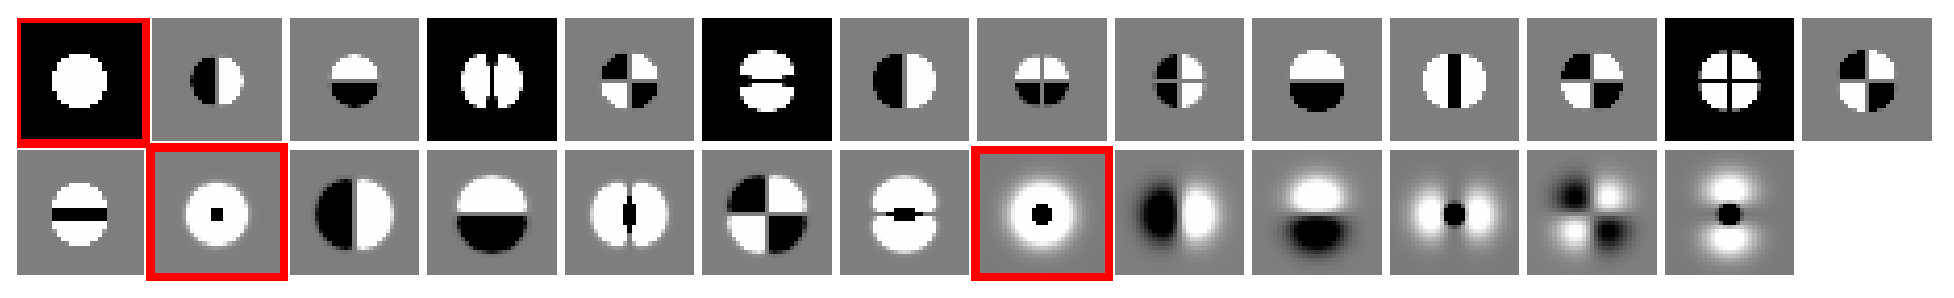
\includegraphics[width=0.8\textwidth]{figures/basis3.eps}}
\caption{Example basis set with nGauss=3 (highlighted in red),
  sigGauss=(0.5 sig, 1.0 sig, 2.0 sig), and degGauss=4, yielding
  Laguerre polynomials of order (4,2,2).}
\label{basis}
\end{figure}

For each source $j$ returned by DiaCatalogSourceSelector, we created a
{\tt KernelCandidate} instance, which holds substamps of $T_j(x,y)$
and $S_j(x,y)$ centered on the source.  These were used to fit for a
local solution $K(u,v)$; the ensemble of local solutions at each
source's $x,y$ was used to fit for the full spatial solution
$K(u,v,x,y)$.  We emphasize that the dimensions of the substamps are
important.  Note from equation~\ref{eq-soln} that the coefficients
$a_i$ are derived from a convolution of the template substamp with the
kernel basis functions $K_i$.  This convolution means that
kernelSize//2 pixels along each substamp edge are rendered unusable.
To maintain a significant number of pixels in $C_i$, we set the {\tt
  KernelCandidate} dimensions to be twice that of the kernel (i.e. the
number of pixels remaining in $C_i$ is equal to the number of pixels
in the kernel, which is fewer than the number of bases $i$).  For each
{\tt KernelCandidate}, we solved for $K(u,v)$ and create a local
difference image $D_j(x,y)$.  We evaluated several statistics on this
local difference image, normalized by the square root of its variance,
which puts the pixels in units of sigma (see also
Section~\ref{sec-stats}).  We measured the mean sigma, the RMS of this
distribution, the $\chi^2$ of these pixels normalized by the degrees
of freedom (number of pixels in $D_j(x,y)$ minus the number of kernel
bases), and the mean squared error.  These are referred to as the
LOCAL kernel metrics, and reflect how appropriate the chosen kernel
basis is (see again Figure~\ref{fig_galleryBad}).

The ensemble of {\tt KernelCandidates} was then used to constrain a
spatial model of the kernel $K(u,v,x,y)$.  This was done using the
{\tt SpatialCellSet} formalism, whereby the {\tt KernelCandidates} are
distributed across the image in a grid of {\tt SpatialCells}.  This
formalism attempts to distribute constraints on the spatial model
evenly across the image.  At most 3 {\tt KernelCandidates} per {\tt
  SpatialCell} were input to the spatial kernel fit.  For the spatial
kernel model, we assumed that each of the kernel coefficients $a_i$
may be represented by a $N^{th}$ order 2--dimensional Chebyshev.
Normally, we would perform sigma--clipping iterations on candidates
having bad residuals after spatial modeling.  However in this
production we expect that all objects should fit, so we performed no
sigma clipping.  Having generated the full spatial solution
$K(u,v,x,y) = \sum_i a_i(x,y) K_i(u,v)$, we evaluated the kernel
solution at the position of each {\tt KernelCandidate}, created a
difference image using this kernel, and recalculated the metrics
defined above.  These are referred to as the SPATIAL kernel metrics.
Importantly, we also interpolated this solution to the positions of
the control sample, which were explicitly {\it not} used in the
spatial fit, and evaluate these same metrics.  The differences between
the {\tt KernelCandidate} LOCAL and SPATIAL metrics, as well as the
values of the SPATIAL metrics for the control sample, reflect the
appropriateness of the spatial model and our ability to interpolate
and extrapolate to the full extent of the images.  We used the Mean
Square Error (MSE) of the control sample to example the tradeoff
between bias and variance in the spatial interpolation.

We next ran the SourceDetectionTask on the difference image, using a
``polarity'' of {\it both} to search for both positive and negative
deviations.  We initially used a nominal detection threshold of 5
sigma.  In the case of pre--filtering, we detected on the difference
image directly.  In post--filtering, we correlated the difference
image with its PSF (by design, the same as the PSF of $S$) before
detection.  All else being equal, the images immediately preceding the
detection step ($D'$) should be {\it exactly} the same.  Detections
were merged using a grow radius of 2 pixels.

Finally, we ran DipoleMeasurementTask on the detections to create {\tt
  DiaSources}.  DipoleMeasurementTask is an extension of
SourceMeasurementTask that includes specific dipole measurement
algorithms.  Measurement was necessarily different in the
pre--filtered and post--filtered data.  In particular, in
post--filtering, detection happens on the filtered maximum likelihood
image and measurement on the associated pixels in the unfiltered
difference image.  In pre--filtering, the latter image does not exist,
and thus detection and measurement happen on the same image.  This
restricts the types of measurements that may be made on the sources
(see Section~\ref{sec-meas}).  While these measurements were
straightforward to implement, additional work needs to be done on how
to implement the remainder of the measurement suite on post--filtered
data (e.g. shapes, moments, and PSF goodness--of--fit metrics).

All {\tt DiaSources} were associated with the {\tt calexp's} sources
and with the reference catalog, with a matching radius of 3''.  {\tt
  DiaSources} that matched with sources may be true residuals around
stars {\it or} true false positives that are also found in the {\tt
  calexp} SourceDetectionTask.  For this reason, we used the
associations with the reference catalog objects as the assessment of
if a given {\tt DiaSource} matched with an input object or whether it
was an orphan (e.g. a statistical fluctuation in the background).  In
addition, all {\tt KernelCandidates} were persisted with the above
{\tt LOCAL} and {\tt SPATIAL} metrics.  Repositories were accessed
with a specially written RepositoryIterator that aggregates {\tt
  KernelCandidates} from a given source across multiple output
repositories.  Finally, the {\tt DiaSource} lists for all production
repositories were compared to find the configurations that yielded the
lowest numbers of false detections.

\subsection{Improvements to Measurement \label{sec-meas}}

We measured flux of {\tt DiaSources} on postfiltered difference images
using PSF--weighted flux photometry (as implemented in the LSST
measurement algorithm "flux.psf").  For measuring fluxes of point
sources on prefiltered images we implemented a new algorithm
"flux.filtered", which works as follows:
%
\[flux = \frac{\sum_{(x,y)}I(x,y) * \phi(x,y)}{\sum_{(x',y')}\phi^2(x',y')}\]
%

where $I(x,y)$ is the image before PSF filtering and $\phi(x,y)$ is an
image of the PSF centered on the source. This equation assumes an
isolated point source, an assumption that is reasonable for difference
images.  We do not weight by the per--pixel variance to avoid
non--linearity in the flux measurement, at the expense of less precise
measurements.

Filtering is performed by convolving the image with its PSF, so the
peak of the filtered image of a given source is:
%
\[Ipeak_{filt} = \sum_{(x,y)}I(x,y) * \phi(x,y)\]
%
Hence the equation for measuring its flux reduces to:
%
\[flux = \frac{Ipeak_{filt}}{\sum_{(x',y')}\phi^2(x',y')}\]
%
Similarly, the predicted uncertainty of the flux measurement is:
%
\[\sigma = \frac{\sqrt{\sum_{x,y}\sigma{^2(x,y)}\phi^2(x,y)}}{\sum_{x',y'}\phi^2(x',y')}\]
%
where $\sigma{^2(x,y)}$ is the is the per-–pixel variance of the
unfiltered image. This reduces to the following:
%
\[\sigma = \frac{\sqrt{\sigma peak{_{filt}^2}}}{\sum_{x',y'}\phi^2(x',y')}\]
%
where $\sigma peak{_{filt}^2}$ is the value of the variance plane,
after filtering, at the peak of the source.

The center of each source is determined using an LSST adaptation of
the SDSS centroiding algorithm "centroid.sdss". In general the source
will not be centered on a pixel, so "flux.filtered" uses a Lanczos 4
resampling kernel to shift the source to be centered on the nearest
pixel before applying the equations above.

\subsection{KernelCandidate Statistics \label{sec-stats}}

We implemented several diagnostics on the quality of the image
subtractions for a given {\tt KernelCandidate}.  This was done for the
original $T_j(x,y)$ to $S_j(x,y)$ kernel fit, yielding LOCAL quality
statistics.  These were re--evaluated using the spatial kernel model
$K(u,v,x_j,y_j)$ evaluated at the {\tt KernelCandidate} location,
yielding SPATIAL quality statistics.  The task metadata was augmented
with summary statistics of these values (mean, median, RMS), and the
information on each {\tt KernelCandidate} persisted in a new {\tt
  kernelSrc} data product.  We briefly describe more useful of these
statistics below.

The first statistic, KCDiffimStDev, measures the standard deviation of
all the non--{\tt EDGE} pixels in the difference image, normalized by
the sqrt of the variance in the difference image.  In the idealized
case, this value should be 1.0, i.e. pixels in the image are drawn
from a normal (0,1) distribution.  In cases of overfitting or
underfitting, this value will be lower than / higher than 1.0.

We also calculate a reduced $\chi^2_\nu$ value called KCDiffimChiSq.
The numerator of this term is the sum of the squares of the
noise--normalized pixel values.  This sum is normalized by the number
of pixels in the data, minus the number of basis shapes in the kernel
plus 1.

Finally in order to investigate the bias--variance trade--off in the
overall fit, we calculate the mean square error (MSE) of each {\tt
  KernelCandidate's} difference image as statistic KCDiffimMseResids.
We define the bias as $\left| data - model \right|$, the variance as
$\left| (data - model)^2 \right|$, and the MSE as {\tt bias$^2$ +
  variance}.  In this context, the bias is the mean of the difference
image, and the variance is the mean square of the difference image.
Ideally, the MSE gives a means for identifying the location in
parameter space of optimal fitting without overfitting.

For all statistics, we have a FITTED sample, which are the {\tt
  KernelCandidates} that were used to derive the spatial model.
Importantly we also have a CONTROL sample of {\tt KernelCandidates}
that were explicitly held out of the fitting to use as a cross
validation sample.

{\bf MOVE ME}
In each case there is a minimum in the measured MSE of the CONTROL sample suggesting
that the test configs span a sufficient range of complexity in the parameter space to 
go from under to over fitting.  Table \ref{tab-bestconfig_MSE}.

\section{Production Runs}

We ran several pre--productions to tune the following aspects of the
pipeline: the dimensions of the kernels and {\tt KernelCandidates};
the widths of the Gaussians (sigGauss) based on the FWHM of the input
images; and the scaling of the Gaussians ($\beta$) in the basis
sequence.  Figure~\ref{fig_galleryBad} provides a rogue's gallery of
image subtraction failures encountered at this stage, each centered on
{\tt KernelCandidates}, and outlines reasons for each failure.
Figure~\ref{fig_galleryGood} provides a gallery showing what the
results from a successful image subtraction appeared like, for
postfiltering on the {\it top} and prefiltering on the {\it bottom}.

The main production runs included: an outer loop over the use of
pre--filtering or post--filtering for detection; variations of the
complexity of the Kernel basis, including the number of Gaussians
(nGauss = 1,3) and the degree of the modifying Laguerre polynomials
(degGauss = 1..6); and the spatial order of the Chebyshev polynomials
on $a_i(x,y)$ (spatialKernelOrder = 1..6).  The final production run
was labeled {\bf run10}, and data are available on the NCSA compute
cluster\footnote{/nfs/lsst8/becker/sparse\_diffim/production10\_sparse}.

Finally, we ran several post--productions focused on perturbing the
solutions that yielded the fewest numbers of {\tt DiaSources} along specific
dimensions.  This included: the RMS of the WCS solution used by
RegisterTask; including a DC offset in the source positions prior to
RegisterTask, to determine the ability of the kernel basis to
accommodate astrometric misregistration; the size of the {\tt
  SpatialCells} used in the spatial interpolation, which effectively
regulates the numbers of constraints that go into the spatial fit; and
modifying the detection thresholds to determine how the number of
false detections scales with threshold.


\section{Results: False Detection Rate}

\subsection{Theoretical \label{sec-analyticfp}}

\subsection{Empirical}

After running an ensemble of 144 pipeline configurations, we
aggregated the numbers of false detections.  We report here the results for
each of the 3 visits, and for pre-- and postfiltering for
detection.  We cut on {\tt flags.pixel.edge} to remove spurious
detections on the immediate border of the image; other than that we do
no other cuts other than requiring that the {\tt centroid.sdss} is
finite.  We separated the {\tt DiaSources} that match with the reference
catalog (3'' matching radius) from those that don't (referred to as
orphans) to investigate the origins of the detections.  We found no
significant correlation of false detections with sensor within the
raft; therefore we report the aggregate results for all 9 sensors in
the analyses that follow.

A set of ``heat maps'' is presented in Figure~\ref{fp_heatmap}, that
demonstrate the total number of detections across all 9 sensors as a
function of the config parameters spatialKernelOrder and degGauss, for
nGauss = 3.  Qualitatively, these heat maps indicate that a Chebyshev
spatial order greater than 3 is required for all data.  In addition,
with the exception of the deconvolution case (v6866601 and
prefilter=False), the Gaussians need to be modified by Laguerre
polynomials of order 4 or higher.  The minimum of these detection maps
are found using the configs of highest complexity, with a very flat
slope in the number of false detections beyond spatialKernelOrder$>$3
and degGauss$>$3.  There is not much evidence for an upturn in the
numbers of false detections, meaning we have likely not reached the
case of severe overfitting using these configs.

The numbers of false detections in each best case are given in
Table~\ref{tab-bestfp10}.  We undertook a manual inspection of all
difference images to associate the {\tt DiaSources} with sources in the
images, and also use a 3'' association with the input source catalog
to define matches and orphans.  Associations are listed in the
N$_{Match}$ column of Table~\ref{tab-bestfp10}, with the unmatched
false positives in the N$_{Orphan}$ column.  The former are likely to
come from systematics in the subtractions of stars, while the latter
would be due to fluctuations in the background.  We note 2 effects
that may impact N$_{Match}$.  The first is that, with a 3'' matching
radius, 4\% of random fluctuations will by--chance associate with a
Source.  Assuming that N$_{Orphan}$ represents 96\% of the background
fluctuation population, we estimate the number of fluctuations from
that same population that would have associated with Sources as
N$_{Random}$.  Finally, we count all matches that occur within 100
pixels of the image boundary, where we might expect deficiencies in
the various spatial extrapolations (astrometry, backgrounds,
PSF--matching kernels) to yield systematic residuals, as N$_{D<100}$.
Figure~\ref{edgedist} provides the distribution of distances from the
edge of the sensor for all false detections in {\it blue}, with a
random sample of points in the image given in {\it green}.
Uncertainties are plotted using the square root of the number of
points in each bin, and the histograms are normalized to provide a
probability density.  Aside from the deconvolution reduction, we find
no significant correlation of false detections with the boundaries of
the fitting functions.  To the extent that N$_{Random}$ $<$
N$_{Match}$, we have a small residual set of systematic false
detections in our imaging ensemble.  Aside from the deconvolution run,
this is at the level of 10 total false detections over 9 sensors in 5
production runs, or 1 every 4--5 images. {\bf REDO BASED ON SIMON'S REANALYSIS}

We also list the ratio of negatively detected to positively detected
{\tt DiaSources}.  That this ratio is significantly greater than 1.0 in most
cases suggests that there is an over-subtraction of the background in
the process, which biases this ratio (see Section~\ref{sec-bg}).  For
completeness, the optimal configurations yielding these false detection
rates are given in Table~\ref{tab-bestconfig10}.

\section{Results: False Detection Dependencies}

After finding the configurations that yielded the minimal numbers of
false detections, we then perturbed the solutions to examine how the
numbers of false detections scaled with different effects.  This
included, in order of importance for this production: the difference
image detection threshold; the number of {\tt KernelCandidates} going
into the spatial model; and astrometric registration errors.  We also
used the theoretical analysis of the number of false detections
expected in a 4k x 4k image as a function of detection threshold in
Section~\ref{sec-analyticfp}, and examine the requirements this sets
on our ability to model the variance and backgrounds in the images.
We compare the empirical variation of false detections with detection
threshold in our data, and show that our results are consistent with
reaching the systematic floor in these data.

\subsection{Effect of Uncertainty on Measured ${S}\over{N}$ \label{sec-sn}}

Section \ref{sec-analyticfp} discusses the theoretical foundation 
that sets the floor on the number of false positives we expect from a 
pure Gaussian random field.  The number of false positives is a strong
function of the seeing and the confidence level of the detection.  
By comparing the empirical false positive rate to the analytic predictions
we can quantify how close we are getting to the theoretical floor in these
data.  Because the number of false positives is such a strong function of
detection threshold, misestimation of the signal to noise of the detections
has a large impact on how many false positives are observed.  

The Figure \ref{fig-fpthresh} shows the 
effect of misestimating the noise in the detections for each of three different
seeing values (0.6$^{\prime\prime}$, 0.88$^{\prime\prime}$, 1.2$^{\prime\prime}$ respectively).  In each case the top panel shows
the number of additional false positives in an LSST size CCD given a fractional misestimation
of the noise in the image and a detection threshold (recall the baseline numbers are given in 
Table~\ref{tab-fp}).  A 1\% under-estimate of the noise
corresponds to ~4 additional false positives at a threshold of $5\sigma$ in the best seeing case.  
The bottom panel shows 
the effect of over-estimating the noise in the measurement.  The effect is to reduce
the number of false positives.  A 1\% under-estimate of the noise results in 2 fewer false positives
per chip.

%By comparing false positive rates to expected rates from the analytic expressions, we may be able to
%estimate the inherent over/under estimation of the reported variance in the images.

The signal of a detection may also be misestimated by over or under subtracting the background.  
The result of errors in modeling the background is to change the ratio of positive to negative
false detections.  The top pane of Figure \ref{fig-skythresh} shows how the ratio of sources of 
different polarities changes as a function of cutoff threshold.  At a threshold of 5$\sigma$
one can observe 50\% more false detections of one polarity over the other with only a 1\% error in background
modeling.  This, of course, also means that {\it different} false positives are detected than if the
background is subtracted perfectly.

Interestingly, the total number of false detections is not nearly as strong a function of background 
modeling errors.  As the number of one polarity decreases, the number of the other polarity increases
almost in proportion.  This is shown in the bottom panel for Figure \ref{fig-skythresh}.

The fact that the total number of false positives depends strongly on the accuracy of the estimation
of the variance but not the background estimation, coupled with the fact that the ratio of positive to 
negative sources should be unaffected by variance misestimation but is very strongly correlated with 
background modeling, gives us leverage to estimate the overall accuracy of both noise estimation and 
background modeling with a single measurement of the number of positive and negative orphans.


%To estimate the numbers of false detections we would expect in a
%$4000\times4072$ pixel science image with a given FWHM in pixels, we
%do the following.  The theoretical expectations for the number of
%false detections due to random Gaussian fluctuations is outlined in
%\cite{Kaiser-PointSources}.

\subsection{Number of KernelCandidates {\bf ANDYB}}

We effectively decreased the numbers of {\tt KernelCandidates} in the
spatial solution by increasing the size of {\tt SpatialCells} used to
model the solution, while keeping the number of objects used from each
cell the same.  We increased this configuration from the default size
of 128 pixels to (256, 384, 512, 640) pixels.  We tracked the numbers
of false detections, and the number of used {\tt KernelCandidates},
and these curves are displayed in Figure~\ref{cellsize}.  The {\it
  left} panel shows the numbers of false detections, while on the {\it
  right} the numbers of {\tt KernelCandidates} used, summed across all
9 sensors.

We note that in the prefiltered data the numbers of false detections
are not strongly dependent on the number of constraints on the spatial
solution.  For visits v6866601 and v6866603 this number is even seen
to decrease with decreasing {\tt KernelCandidates}.  This suggests
that in prefiltering there is not a significant difference in quality
of fit when using $\sim$600 vs. $\sim$300 {\tt KernelCandidates} per
sensor.  The overall fit is demonstrably worse when using only
$\sim$100 constraints on the model (cell size = 640).  The indication
is that 300 constraints on the spatial model (which has 28, 28, and 21
terms per basis for visits v6866601, v6866602, and v6866603
respectively) appears sufficient in the case of prefiltering.

In the case of postfiltering, aside from the deconvolution case, the
number of false detections continually increases as the number of {\tt
  KernelCandidates} decreases.  This indicates that the best mode to
operate in when postfiltering is to maximize the number of constraints
on the model.

\subsection{Registration Errors}

We implemented two simple perturbations of the inputs to the
image--to--image RegisterTask: we first added a random offset to each
object's (x,y)-coordinates, with an amplitude that was specified in
the Config and multiplied by a random number pulled from a normal
distribution; and we added a DC offset to the coordinates at an
amplitude specified in the Config.  These offsets, added to the Source
coordinates, will cause misalignments of the objects in the registered
images, as the registration is done assuming the specified positions
are correct.  In this way we are able to investigate how random
uncertainties and bulk astrometric offsets impact the false positive
rate.  We explicitly do {\it not} investigate spatial variation in
these offsets, for example using a pincushion distortion.  We
anticipate that this latter effect will be most important for spatial
interpolation and extrapolation of the matching kernel, yielding a
dipole residual field associated with the distortion.  However, we
start with the basics here to investigate the individual terms in such
misalignments.

\subsubsection{Coordinate RMS}

We perturbed the coordinates of each template Source that was input to
RegisterTask with amplitudes of (0.025, 0.05, 0.075, 0.1, 0.125, 0.15,
0.175, 0.2, 0.3, 0.4, 0.5, 1.0, 1.5, 2.0, 2.5, 3.0, 3.5, 4.0) pixels,
and to randomize the effects we multiplied each offset by a number
pulled from a normal (0,1) distribution.  The output RMS reported by
RegisterTask was noted to track these offsets.  

Figure~\ref{wcsrms} shows how the numbers of false positives scales
with this RMS.  Note that the distribution is very flat out to 1.0
pixel (0.2'') for all images except for the deconvolution
configuration.  The number of false positives doubles after an RMS of
1.5--2.0''.  This test indicates that, for this very simplified case,
random astrometric uncertainties do not strongly impact the difference
image quality.  This may change with more realistic distributions of
stellar brightnesses, if individual objects pull the fit more than
others due to inverse variance weighting.  In this production, with the
stars having the same brightness, no single random offset is likely to
drive the fit.

\subsubsection{Coordinate Offsets}

We offset the coordinates of each template Source that was input to
RegisterTask with amplitudes of (0.025, 0.05, 0.075, 0.1, 0.125, 0.15,
0.175, 0.2, 0.3, 0.4, 0.5, 1.0, 1.5, 2.0, 2.5, 3.0, 3.5, 4.0) pixels.
Post--registration, this will offset the positions of sources in the
two images by the desired amount.

Figure~\ref{wcsshift} shows how the numbers of false positives scales
with this shift.  Surprisingly, the distribution is very flat out to
nearly 1.0 pixels (0.2'') for all images except for the deconvolution
configuration.  The number of false positives doubles after a shift of
1.5''.  This test indicates that, for this very simplified case, bulk
astrometric offsets of the degree expected from nightly processing
should not drive the false positive rate.  

Figure~\ref{kernel_offsets} demonstrates the ability of the
PSF--matching kernel to redistribute flux to account for bulk
astrometric misalignments.  Since these offsets are common--mode
amongst all {\tt KernelCandidates}, the basis shapes themselves drive
the pipeline's ability to compensate for them.  Having a Gaussian
basis function whose sigma is commensurate with the amplitude of the
offset enables the software to place significant power in this basis
term.  We expect that, if these misalignments are a vector field, the
ability of the spatial kernel model to account for the spatial
variation of the misregistration will begin to drive the solution.
The take--away from this analysis is that the PSF--matching basis
appears flexible enough to account for, individually, random scatter
and bulk offsets in the WCS solution.  This narrows the focus down to
understanding how spatial variation in the WCS--based registration may
drive the difference image quality, and what requirements need to be
put both on the kernel basis and its spatial variation.


\subsection{Variance Misestimation}

{\bf good point: note that the curves nfp vs. threshold are
  correlated, its a cumulative distribution}.

Because these images will have gone through multiple convolutions
before reaching the detection stage, it is expected that the
propagated per-pixel variance will not provide an exact representation
of the empirical variance in the image planes \citep{Price-Stacking}.
Because the astrometric resampling uses a warping kernel that is
designed to preserve the noise properties of the images, we expect
that the kernel convolution and PSF--filtering will provide the largest
sources of error.

To quantify these errors, we first compared the empirical variance in
the image planes with the level tracked by the variance planes.  We
calculated the ratio of the interquartile range of unmasked pixels in
the image plane, multiplied by 0.741 and then squared, with the median
of unmasked pixels from the variance plane.  The former represents the
empirical variance, while the latter the propagated variance.  We
investigate their ratio (empirical/propagated) at 2 stages in the
processing: after creation of the difference image (image $D$), and
immediately preceding detection (image $D'$).  Recall that for
prefiltering, $D = D'$.  These results are summarized in
Table~\ref{tab-variance1}.  For prefiltering, we find that the
variance plane typically underestimates the true variance by $1\%$ for
all visits.  When using postfiltering, the deconvolution visit
v6866601 yields a similar underestimate in the difference image, but
for the other two visits the variance is tracked to better than 1\%,
with a small RMS.  However, when postfiltering with the PSF, the
variance becomes {\it overestimated} by nearly a factor of two for
deconvolution visit v6866601, and {\it underestimated} by $4-5\%$ for
the other visits.

We next investigated the variance properties of the images that are
input to the detection stage, i.e. the difference image itself in the
case of prefiltering, and the difference image correlated with its PSF
in postfiltering.  These results are summarized in
Table~\ref{tab-variance2}.  We find that the image planes have very
similar empirical noise properties at the detection stage, with the
deconvolution visit having larger variance by $1\%$ but the other
visits having essentially equal noise properties, with a bias towards
the postfiltered data having slightly higher variance (while the RMS
is small, all values are greater than 1.0)\footnote{For completeness,
  we note the median differences between the image planes at the time
  of detection are 3--4 counts (or 0.2 sigma relative to the empirical
  variance) for v6866601, 0.2 counts (0.02 sigma) for v6866602, and
  less than 0.1 counts (0.01 sigma) for v6866603.}.  The medians of
the variance planes tell a different story though.  For the
deconvolution visit, the median per--pixel variance is $70\%$ higher.
While this will suppress the detections of false positives, it will
also significantly suppress the detection efficiency for true
variability.  For the other visits, the postfiltered per--pixel
variance is relatively {\it lower} by $3-4\%$.  This will increase
the sensitivity of the postfiltered data to false positives; as shown
above, the rate is indeed larger using the postfiltering pipeline.
This analysis demonstrates that this is primarily due to an {\it
  underestimate} of the per--pixel variance in the postfilter
processing: while the prefiltered variance is a 1\% underestimate, the
postfiltered variance is a 5\% underestimate.  As outlined by
\cite{Price-Stacking}, this may be due to loss of pixel covariance
when undergoing multiple convolutions, as covariance is not currently
tracked in the DM stack.  In prefiltering, the science image undergoes
a single convolution, and the template image a single convolution.  In
postfiltering, the template image undergoes a convolution, is
subtracted from the science image, and then undergoes a second
convolution with the Psf.  As we have demonstrated here, this second
convolution is where our variance bookkeeping lags the empirical
variance.

\subsection{Detection Threshold}
Obviously the number of false positives is strongly dependent on the detection threshold.  In order to
check the scaling of our false positive rates with detection threshold, we ran the same config (see \ref{tab-bestconfig10} 
for the config parameters)
at several detection threshold values for each visit both prefiltering and postfiltering.  As discussed in 
Section~\ref{sec-analyticfp} one can predict the number of false positives expected in a sensor given
seeing and threshold values.  Some example values of the number of false positives (both +ve and -ve)
expected in LSST size detectors are given in Table \ref{tab-fprate}.  

As discussed in the Section \ref{sec-sn}, the accuracy of the noise estimation in the detection is crucial to 
understanding the false positive rate.  In the previous section we quantify the under--estimation of the variance
by the variance plane in the case of pre and post filtering.  In our analysis of the threshold dependence of
our false detection rate we must correct for this under--estimation in order to put the counts from each algorithm
on the same normalization.

Figure \ref{fig-fp_v_thresh} shows the results of this analysis.  In all figures red squares are postfiltered data and
blue circles are for the prefiltering technique.  All values are for the number of false positives in a 4000x4072 sensor.
Using a Monte Carlo approach we 
estimate the variance on the predicted false positive rate as a function of threshold.  The 1-$\sigma$ confidence envelope is shown
as shaded grey about the model line in dark black.  From left to right the panels are for v6866601 -- 0.6$^{\prime\prime}$ FWHM,
v6866602 -- 0.88$^{\prime\prime}$ FWHM and v6866603 -- 1.2$^{\prime\prime}$ FWHM respectively.  Except in the case of deconvolution
in the postfiltering case (v6866601) the count rates between the two algorithms agree very well when corrected for the
observed under--estimation of the noise by the variance plane.  In the case where postfiltering requires a deconvolution, the high $\over{S}{N}$
detections come primarily from detection of the ringing around stars.

In all cases the empirical results are below the predicted results indicating
that the number counts are smaller than the theoretical floor.  {\bf What should we say about this here?} We can correct for this by scaling
the prediction by 2.5\%, 1.5\% and 1\% for v6866601, v6866602, and v6866603 respectively.  The data plotted with these corrections are shown
in the bottom row.  Once this correction is done, the trend of false positive rate with detection threshold agrees to within 1-$\sigma$ for the 
prefiltering case for all three seeing values.

\section{Results: Correlation with KernelCandidate Statistics}

In Figures~\ref{corrpre} and \ref{corrpost} we correlate statistics
calculated on the control sample of {\tt KernelCandidates} with the
numbers of false detections that come out of detection and
measurement, for the prefiltering and postfiltering cases
respectively.  We do this for statistics that represent the median
standard deviation of the pixels in the {\tt KernelCandidate} SPATIAL
difference image (KCDiffimStDev), the median reduced chi2 of the
pixels in the difference image (KCDiffimChiSq), and median MSE of the
residuals (KCDiffimMseResids).  These values are defined in
Section~\ref{sec-stats}.  There is one point in each figure from each
sensor in each of the 72 production runs per prefilter and postfilter
configuration.

For postfiltering, Figure~\ref{corrpost} indicates that these metrics
correlate strongly with each other, meaning there is likely little
advantage to looking at more than one metric.  The deconvolution visit
in {\it red} is a clear outlier in this distribution.  While there is
a relationship between the values of these metrics and the numbers of
false positives, it is relatively flat until $\sim 10^2$ false
detections per sensor; the scatter below this threshold is similar to
the trend, meaning there is no single metric studied that may be used
to predict the numbers of false detections during the fitting process,
within the range of interest ($<10$ false detections per sensor).

For prefiltering, Figure~\ref{corrpre}, the slope between $10^0$ and
$10^1$ false detections is steeper, but still commensurate with the
scatter within that range.  The metrics are still strongly correlated
with each other, but not to the degree as for the postfiltered
statistics.  A less--noisy relationship may be obtained through a
linear combination of these metrics, but we have not fully
investigated this option.  As a summary, these statistics clearly
correlate with the numbers of false positives, and we plan to quantify
these correlations in further detail as we continue our work in Summer
2013.

Using this simplified data set, we can begin to look at how we may predict 
optimal configs based measured statistics.  We notice that the MSE of the
control sample has a minimum in all cases.  See Figures \ref{fig-MSE_CONTROL}
and \ref{fig-MSE_FITTED} to see the behavior of the MSE for the control sample and
fitted sample respectively.  We note that the config at the minimum MSE value is
not always the same config.  Table \ref{tab-bestconfig_MSE} lists the configs
at the minimum of the MSE for the control sample.  This can be compared to
the configs in Table \ref{tab-bestconfig10}.

Since we were looking as MSE values for all chips at once, it's possible that
each sensor has it's own optimal config and thus the aggregate MSE is not a 
good indicator of overall config optimization.  To get a handle on this, we
looked at per sensor MSE values and per sensor false positive rates.  In fact,
the config that produces the minimum number of false positives is variable
from sensor to sensor.  It is worth investigating how much the false positive rate
per chip goes down if per sensor optimal configs are used instead of per visit optimal
configs.

When we look at the MSE per chip and compare with the minimum false positive config we 
find good agreement.  The findings are summarized in Table \ref{tab-MSE_persensor}.  Because
the MSE is sensitive to over fitting, we observe that it tends to lower complexity configs
even if the false positive rate is slightly higher.

However, the trends are encouraging and we will pursue these methods
in our future work with the more complicated simulations.

\section{Results: Measurement}

Figure~\ref{fluxerr} provides a mosaic of absolute--value S/N
measurements for the {\tt DiaSources} detected at 5--sigma.  The {\it
  top} panel shows the PSF flux measurements reported in the
postfiltered analysis, while the {\it bottom} panel shows the filtered
flux measurements in the prefiltered analysis.  Both distributions are
strongly peaked at 5--sigma, indicating we are not grossly
mismeasuring fluxes or flux uncertainties in either case.

\section{Results: Computational Performance}

For this production, the understanding of the algorithm and
optimization of the false detection rates took priority over
optimizing the computational performance of the algorithms.  In
particular, debugging hooks were implemented and workarounds of
problems were devised with the focus on understanding the core
PSF--matching algorithm.  Therefore there are several key ways in
which the production as--implemented will differ from how the code is
used in Nightly and Data Release Processing.  We outline these
differences below.

The first difference is that due to problems with the {\tt
  meas\_astrom} package, detailed in Section~\ref{subsec-astrom}, we
were unable to exercise the envisioned data flow where we query a
coadd repository for the template image.  Instead we used a single
deep {\tt calexp} as the template image.  The astrometric registration
of these images was trivial, as the images almost exactly overlap and
are exactly the same size.  Thus the timings of the {\tt
  imageDifference:register} task are {\it underestimates} of the
expected astrometric registration subtask computational performance.

Second, the core performance of the {\tt imageDifference:subtract}
task will be significantly impacted by debugging hooks that were put
in place specifically to generate the metrics being evaluated in this
production.  The core functionality, {\tt matchMaskedImages}, does the
convolution kernel fitting and actual convolution of the template
image, and will be least impacted by these add--ons.  The reported
timings of {\tt matchMaskedImages} are thus an {\it overestimate} of
the method's performance.

The reported {\tt imageDifference:detection} task performance is an
accurate representation of its computational requirements.  However,
the {\tt imageDifference:dipolemeasurement} task represents a
significant overestimate of the true dipole measurement requirements.
In particular, the PSF--flux dipole measurement is explicitly
sub--optimal, in that its centroid fitting algorithm is a 4--deep {\tt
  for} loop.

With these caveats, the timings of the {\tt imageDifference} subtasks
are presented in Table~\ref{tab-timings}.

\section{Conclusions}

{\bf DOUBLE CHECK THESE WHEN THE DUST SETTLES}

\begin{itemize}

\item We can reach near the theoretical limit for false detection rate
  in these ideal data, something which has not been demonstrated for
  image subtraction algorithms in the past.

\item Pre--filtering is clearly preferred when the traditional process
  would lead to deconvolution, or sharpening, of the data.  When the
  standard processing results in a convolution, or smoothing of the
  data, pre--filtering provides fewer false detections.  As a
  trade--off, the measurement of these false detections is not yet
  well defined.

\item We find that the overall number of false detections is not
  strongly sensitive to bulk background misestimation
  (Figure~\ref{XXX});

\item However, the ratio of positive to negative false detections is
  strongly dependent on background fitting, with {\bf XXX}
  (Figure~\ref{XXX}).


and \ref{fig-MSE_FITTED} to see the behavior of the MSE for the control sample and
fitted sample respectively.  We note that the config at the minimum MSE value is
not always the same config\item Our empirical negative to positive false detection ratio is {\bf
  X.X}, indicating a bias in the background levels of {\bf X\%}.

\item At the 5--sigma detection threshold, for the range of seeings
  considered in this production, the theoretical numbers of false
  detections per 4k x 4k sensor numbers 10+.  This function is steep;
  by increasing the detection threshold to 5.X sigma this number may
  be lowered to less than 1 per sensor.

\item Due to the steepness of this function, the number of false
  detections is strongly dependent on the variance being correct, at
  the 5--sigma detection threshold.  When detecting at 5--sigma,
  having the variance underestimated by 1\% leads to an increase
  in false positives of {\bf XXX} (Figure~\ref{}).

\item An empirical computation of the variance from the image plane,
  compared to the median propagated variance in the variance plane,
  indicates that we consistently underestimate the variance in
  prefiltering by $1-2\%$, and in postfiltering by $4-5\%$ when not
  strongly deconvolving (Table~\ref{tab-variance1}).  The latter
  effect is shown to arise from the PSF--filtering of the difference
  image immediately before detection.  This is likely due to the
  double--convolution that is happening to the template image, and our
  having no current mechanism to track pixel covariance.

\item The empirical variance of the detection images in prefiltering
  and postfiltering are similar to within $1\%$
  (Table~\ref{tab-variance2}).  However, the variance in the
  postfiltered data is $3-4\%$ {\it lower} in the postfiltered data,
  leading to a larger number of false positives when using the
  variance plane as the definition of sigma.

\item When strongly deconvolving, the postfiltered variance is 70\%
  {\it higher} at the time of detection compared to the prefiltered
  data (Table~\ref{tab-variance2}).  This is consistent with the
  understanding that deconvolution increases high frequency noise in
  the images, and provides a {\it lower} detection efficiency in
  deconvolved data.  Prefiltering is clearly preferred in the case of
  significant deconvolution (v6866601).

\item The postfilter pipeline can produce difference images with a
  minor deconvolution (v6866602) at a quality commensurate with a subtraction that uses a
  smoothing convolution (v6866603).

\item The false detection rate is seen to scale with detection
  threshold in a manner consistent with theory (Figure~\ref{}).

\item The measurement of {\tt DiaSources} detected at 5--sigma are
  shown to have a commensurate measured signal--to--noise
  (Figure~\ref{fluxerr}).  

\item Measurements on prefiltered difference images contain less
  information than in postfiltered difference images, because the
  paradigm of detection on filtered data but measurement on the
  unfiltered data is broken.  Thus while we detect on average fewer
  false positives in prefiltered data, we are (so far) able to
  characterize them less well.  This trade--off is clearly something
  to explore in future work.

\item Several statistics that we are able to calculate at the time of
  image subtraction are shown to correlate strongly with the numbers
  of false detections (Figure~\ref{corrpost} and
  Figure~\ref{corrpre}).  However, these relationships have a shallow
  slope in the area of interest (number of false detections per sensor
  less than 10).  Additional work will be required to produce a robust
  predictor of false positive rate.


\end{itemize}

\section{Outstanding Issues}
We ran into some issues during this production that required work--arounds.  
In some cases we did not have the time to drill all the way down
to the root cause.  We itemize these issues here so that they may be addressed 
as part of the Summer 2013 work.


\subsection{Astrometric Registration \label{subsec-astrom}}
The original plan for this production was to use the single deep exposures (v6866600) as 
inputs to the coadd process, to exercise use of the coadd repository.  As 
such we warped the exposures to coadd patches for use in the image difference
task.  The register task was unable to solve a differential WCS between the coadd
and science {\tt calexp} because in coadds, the parent WCS is for the entire {\tt tract}.
Each coadd {\tt patch} thus has a CRPIX at the center of the {\tt tract}, which is
typically off the {\tt patch} image.  TAN--SIP is unable to perform in this circumstance,
as it expands its polynomials around the CRPIX.  To get around this 
we tried re--solving the coadd patches using a TAN--SIP solution that was solved from
scratch.  This worked fairly will part of the time,
yielding residuals in the 40--100 mas range, compared to the 250 mas previously.  However,
as we did not understand the origin of these problems, and there were legitimate bugs
in meas\_astrom  that were uncovered as a result of this investigation, we reverted to
using the deep {\tt calexp} as the template directly; the direct deep {\tt calexp} to science {\tt calexp} 
registration typically yielded residuals in the range of 4--5 mas.

We investigated potential causes of the large residuals.  To do this, we looked at the 
residuals for template--to--refcat solutions, science image--to--ref solutions, and 
direct template to science image registration to attempt to isolate where the astrometry 
was being degraded.  The results are shown
in table \ref{tab-wcsrms}.  We show the results for the nine sensors in the best seeing visit.  

The solutions for the three steps that do not involve any warping show results consistent with 
the accuracy we expect to get.  We also see the expected trend that the deep exposures have 
smaller RMS than the solutions of the science images.  The coadd--to--science registration
depends critically on the WCS fitting and warping process: the WCS of the deep {\tt calexp} is warped
into the coadd {\tt patch}; the coadd {\tt patch} is then warped into the science {\tt calexp} frame.
This places two dependencies on the warping code, and two on the WCS fitting, where
this degradation may have occurred.

\subsection{Detection and Measurement on Negative Sources}
We see more negative false detections than positive false detections.  This drove an investigation 
into the symmetry of detection and measurement on positive/negative sources.  To do this we looked at the 
results of the image difference task and compared it to the same runs when the difference image was inverted
(multiplied by -1) before measurement.  The results are as follows:
\begin{itemize}
\item Centroids of negative sources always have integer of half--integer values.
\item The {\tt DiaSource} lists are always the same length.
\item Centroiding on negative sources fails almost all the time: 99.7\% sources with negative flux
have the {\tt badcentroid} flag set.
\item psfFlux can be measured at 0. even when no flags are set.
\item psfFlux can be measured as NaN with valid centroid values and no other flags set.
\item psfFlux can have the same sign in both the initial and inverted image 0.1\% of measurements.
\item Some sources are have the {\tt EDGE} bit set at one polarity but not the other.  
  This leads to a difference in the reported number of false positives as we only consider 
  those without the {\tt EDGE} flag set.
\end{itemize}

The suspicion is that the differences in the precision of the centroids is linked to the differences in flags.
We have not had the time to chase this down completely, but plan on doing so in Summer 2013.


\section{Future Work}

We intend to research additional aspects of the problem going forward,
including:
\begin{itemize}
\item How the false detection rate varies with more realistic SEDs;
\item How the false detection rate varies with airmass;
\item How the system behaves with a realistic mix of stars and galaxies;
\item How the false detection rate looks in crowded fields;
\item Adoption of Gaussian processes for spatial modeling of the kernel;
\item Investigating the differences in measurement on positive/negative sources;
\item Developing a measurement suite (shape, moment, goodness of fit) for sources in prefiltered data;
\item Determining how much ``on the fly'' configuration we may do to optimize PSF--matching.
\end{itemize}

\clearpage
\bibliographystyle{apj}
\bibliography{refs}

\clearpage

\begin{table}
\centering
\begin{tabular}{lcc}
\hline
\multicolumn{3}{|c|}{Theoretical Number of False Detections per Sensor} \\
\hline
Visit    & FWHM (pixels) & N\\
\hline
v6866601 & 3.0 & N \\
v6866602 & 4.4 & N \\
v6866603 & 6.0 & N \\
\end{tabular}
\caption{Total number of false detections that we expect based on
  {\bf blah}.  We list the total number of positive {\it plus} negative detections;
  they should be present in equal quantities. \label{tab-fp}
}
\end{table}



\begin{table}
\centering
\begin{tabular}{clcccccc}
\hline
\multicolumn{8}{|c|}{Best Results: Production 10} \\
\hline
Visit    & Prefilter & Total False Detections &  N$_{Orphan}$ & N$_{Match}$ & N$_{Random}$ & N$_{D<100}$ & Nneg / Npos \\
\hline
v6866601 & True      & 70      &60         & 10 & 3     & 4   & 1.8 \\ 
         & False     & 143     &51         & 92 & 2     & 11  & 0.4 \\
v6866602 & True      & 42      &36         & 6  & 2     & 1   & 2.6 \\
         & False     & 53      &45         & 8  & 2     & 1   & 0.5 \\
v6866603 & True      & 23      &23         & 0  & 1     & 0   & 2.8 \\
         & False     & 36      &35         & 1  & 1     & 0   & 3.4 \\
\end{tabular}
\caption{Total number of {\tt DiaSources} detected at 5--sigma from
  all 9 sensors in raft 2,2, for the configurations that yielded the
  lowest number of false detections.  Matches are determined using a
  3'' match radius with the input reference catalog.  Objects with the
  {\tt EDGE} flag are ignored.  We list the number of background
  fluctuations that are expected to randomly associate with a Source
  N$_{Random}$, given the density of objects in the images and a 3''
  match radius, assuming that N$_{Orphan}$ represents 96\% of the
  total population of detections from Gaussian fluctuations.
  We also list the number of false detections that are found within
  the outer 100 pixels of the image N$_{D<100}$.  The final column
  lists ratios of the number of negatively detected false detections
  to those with positive flux, a 5--sigma. \label{tab-bestfp10}}
\end{table}


\begin{table}
\centering
\begin{tabular}{clccc}
\hline
\multicolumn{5}{|c|}{Best Configs: Production 10} \\
\hline
Visit    & Prefilter & nGauss & degGauss & spatialOrder \\
\hline
v6866601 & True      & 3      & 6        & 6 \\
         & False     & 3      & 1        & 5 \\
v6866602 & True      & 3      & 6        & 6 \\
         & False     & 3      & 6        & 5 \\
v6866603 & True      & 3      & 5        & 5 \\
         & False     & 3      & 4        & 6 \\
\end{tabular}
\caption{Configurations that led to the best results listed in
  Table~\ref{tab-bestfp10}.  All post-production runs include
  perturbations about these configurations. \label{tab-bestconfig10}}
\end{table}

\clearpage

\begin{table}
\centering
\begin{tabular}{clccc}
\hline
\multicolumn{5}{|c|}{Best Configs: From Minimum MSE} \\
\hline
Visit    & Prefilter & nGauss & degGauss & spatialOrder \\
\hline
v6866601 & True      & 3      & 4        & 5 \\
         & False     & 3      & 1        & 6 \\
v6866602 & True      & 3      & 4        & 6 \\
         & False     & 1      & 3        & 5 \\
v6866603 & True      & 3      & 5        & 5 \\
         & False     & 3      & 5        & 5 \\
\end{tabular}
\caption{The best configs as derived from the minimum in the measured MSE.  It should 
be noted that the minimum is fairly shallow.
\label{tab-bestconfig_MSE}}
\end{table}

\clearpage

\begin{table}
\centering
\begin{tabular}{clccc}
\hline
\multicolumn{4}{|c|}{Variance Ratios: Empirical / Propagated} \\
\hline
Visit    & $D_{pre} = D'_{pre}$ & $D_{post}$ & $D'_{post}$ \\
\hline
v6866601 &$1.012 \pm 0.002$&$1.018 \pm 0.005$&$0.599 \pm 0.017$ \\
v6866602 &$1.010 \pm 0.002$&$1.007 \pm 0.001$&$1.046 \pm 0.002$ \\
v6866603 &$1.015 \pm 0.003$&$1.008 \pm 0.001$&$1.045 \pm 0.003$ \\
\end{tabular}
\caption{Ratio of the empirical variance in the difference images,
  calculated via (0.741 times the interquartile range)$^2$, to the
  median of the variance plane.  In all cases (except the deconvolution configuration) the variance plane
  represents an {\it underestimate} of the true variance in the
  images.  We report the mean and RMS across all sensors for the best
  configurations.  }
\label{tab-variance1}
\end{table}

\begin{table}
\centering
\begin{tabular}{ccc}
\hline
\multicolumn{3}{|c|}{Variance Ratios: $D'_{post} / D'_{pre}$} \\
\hline
Visit    & Empirical & Propagated \\
\hline
v6866601 & $1.011 \pm 0.016$    & $1.710 \pm 0.049$    \\
v6866602 & $1.001 \pm 0.001$    & $0.967 \pm 0.001$    \\
v6866603 & $1.002 \pm 0.001$    & $0.974 \pm 0.002$    \\
\end{tabular}
\caption{Ratios of the variance planes immediately before detection
  $D'$.  Ratios are in the sense of the variance of the postfiltered
  image divided by the variance of the prefiltered image.  The first
  column represents the ratios of the empirical variance, calculated
  via (0.741 times the interquartile range)$^2$.  The second column
  reports the ratios of the medians of the propagated variance planes.
  We report the mean and RMS across all sensors for the best
  configurations.}
\label{tab-variance2}
\end{table}


\clearpage
\begin{table}
\centering
\begin{tabular}{|c|c|c|c|c|}
\hline
\multicolumn{5}{|c|}{WCS RMS in mas at various stages} \\
\hline
Sensor    & Deep & Science &  Deep to Science & Coadd to Science \\
\hline
R22:S00&4.2&5.8&3.8&382\\ 
R22:S10&2.6&4.4&4.4&389\\
R22:S20&1.4&3.6&4.2&375\\
R22:S01&2.6&5.0&4.2&86\\
R22:S11&1.2&3.4&4.0&81\\
R22:S21&1.6&3.8&4.0&382\\
R22:S02&1.6&3.4&4.0&178\\
R22:S12&1.8&4.0&4.0&78\\
R22:S22&1.4&4.2&4.2&389\\
\hline
\end{tabular}
\caption{We looked at the resulting RMS from WCS fitting on the source lists of the deep exposure to the reference catalog, the science exposure to the reference catalog,
fitting the deep exposure directly to the science exposure, and fitting a warped coadd to the science exposure.  Fitting 
the coadd to the science exposure produces an order of magnitude more scatter in the fit than at any other point. {\bf SIMON MAKE SURE NUMBERS ARE STRAIGHT}\label{tab-wcsrms}}
\end{table}
\clearpage


\begin{figure}
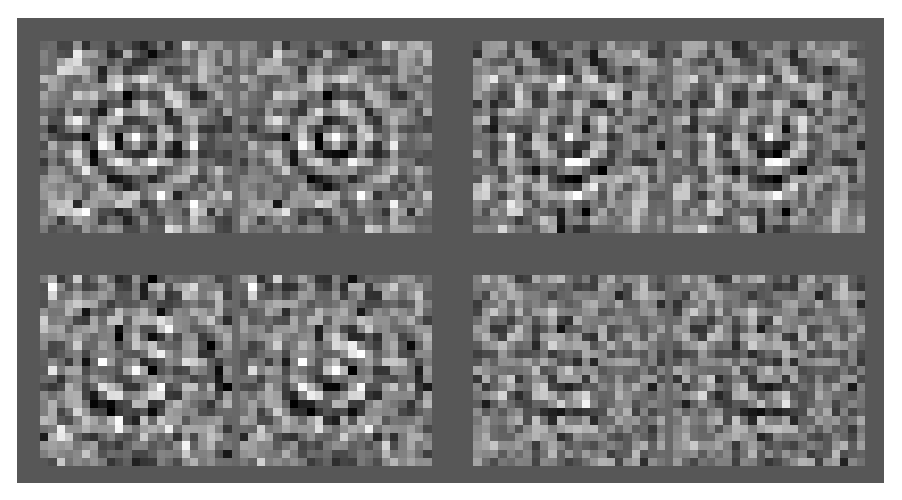
\includegraphics[width=0.5\textwidth, height=0.25\textwidth]{figures/deconv2.eps} 
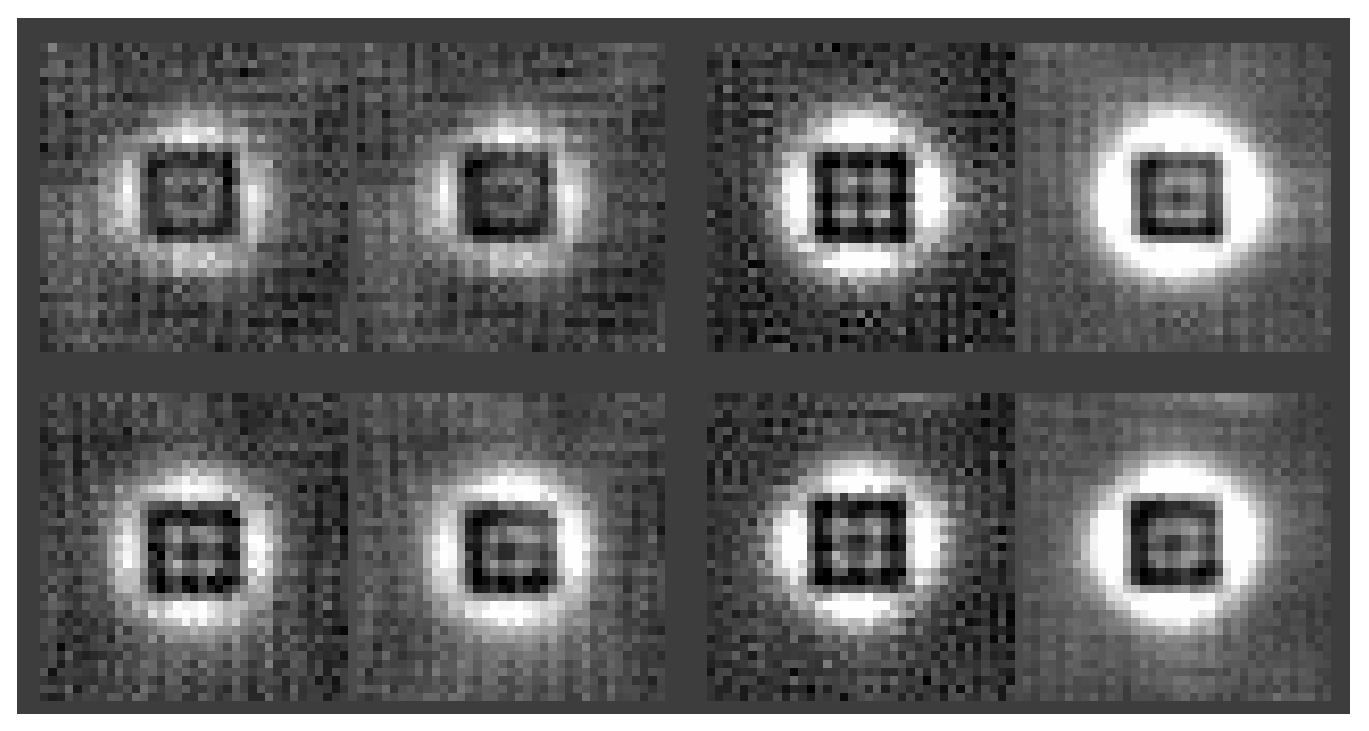
\includegraphics[width=0.5\textwidth, height=0.25\textwidth]{figures/size2.eps} \\
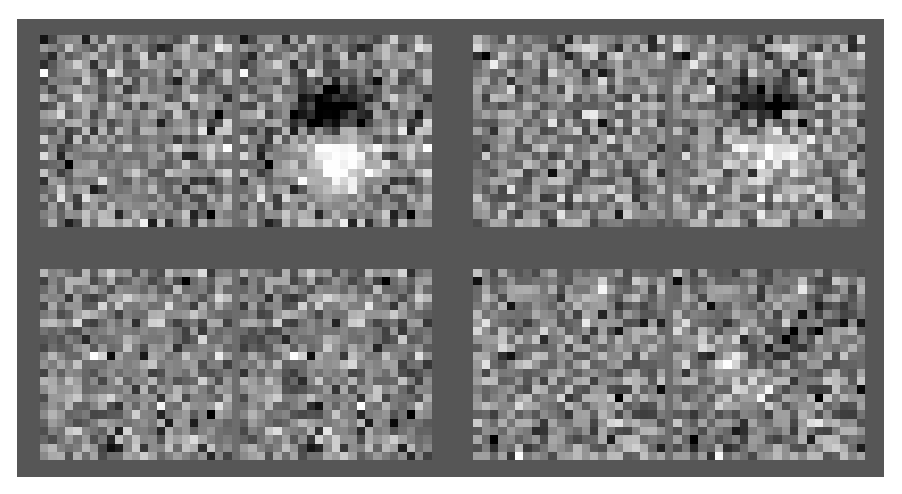
\includegraphics[width=0.5\textwidth, height=0.25\textwidth]{figures/order2.eps} 
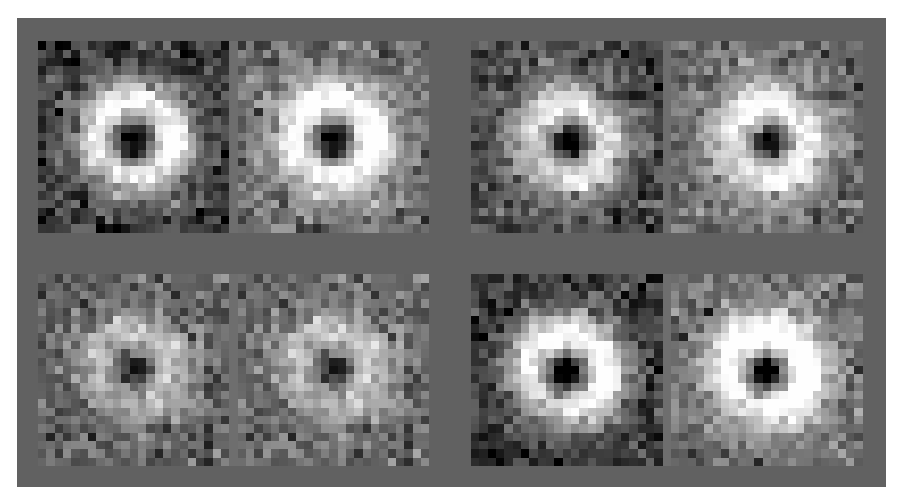
\includegraphics[width=0.5\textwidth, height=0.25\textwidth]{figures/shape2.eps} \\
\caption{Four example panels showing failure modes of the image
  subtraction software.  Each panel itself shows a 2x2 pair of
  {\tt KernelCandidate} difference images; on the {\it left} subpanel is the residual from
  the LOCAL fitting, and on the {\it right} from the SPATIAL fitting.
  Starting in the upper left and going clockwise, the first panel
  shows the residuals when deconvolving the template image; the
  ringing is characteristic of the deconvolution process.  Next, a set
  of difference images where the kernel dimensions (kernelSize) are
  too small to match the sources, leaving square kernel--sized
  residuals around each object.  Next, a set of images where the
  kernel shape (sigGauss) is inappropriate to match the sources; note
  that the LOCAL residuals show circular residuals, indicating the
  basis set itself is at fault (as opposed to the spatial model).
  Finally, in the lower--left, a set of images that demonstrate how
  the residuals degrade when the spatial kernel model is at fault.
  Note that the LOCAL residuals appear to be white noise, while the
  SPATIAL residuals show a clear dipole signature.  For this reason, a
  comparison between the LOCAL and SPATIAL residuals is a useful
  diagnostic of the spatial model.  }
\label{fig_galleryBad}
\end{figure}

\begin{figure}
\begin{center}
\centering{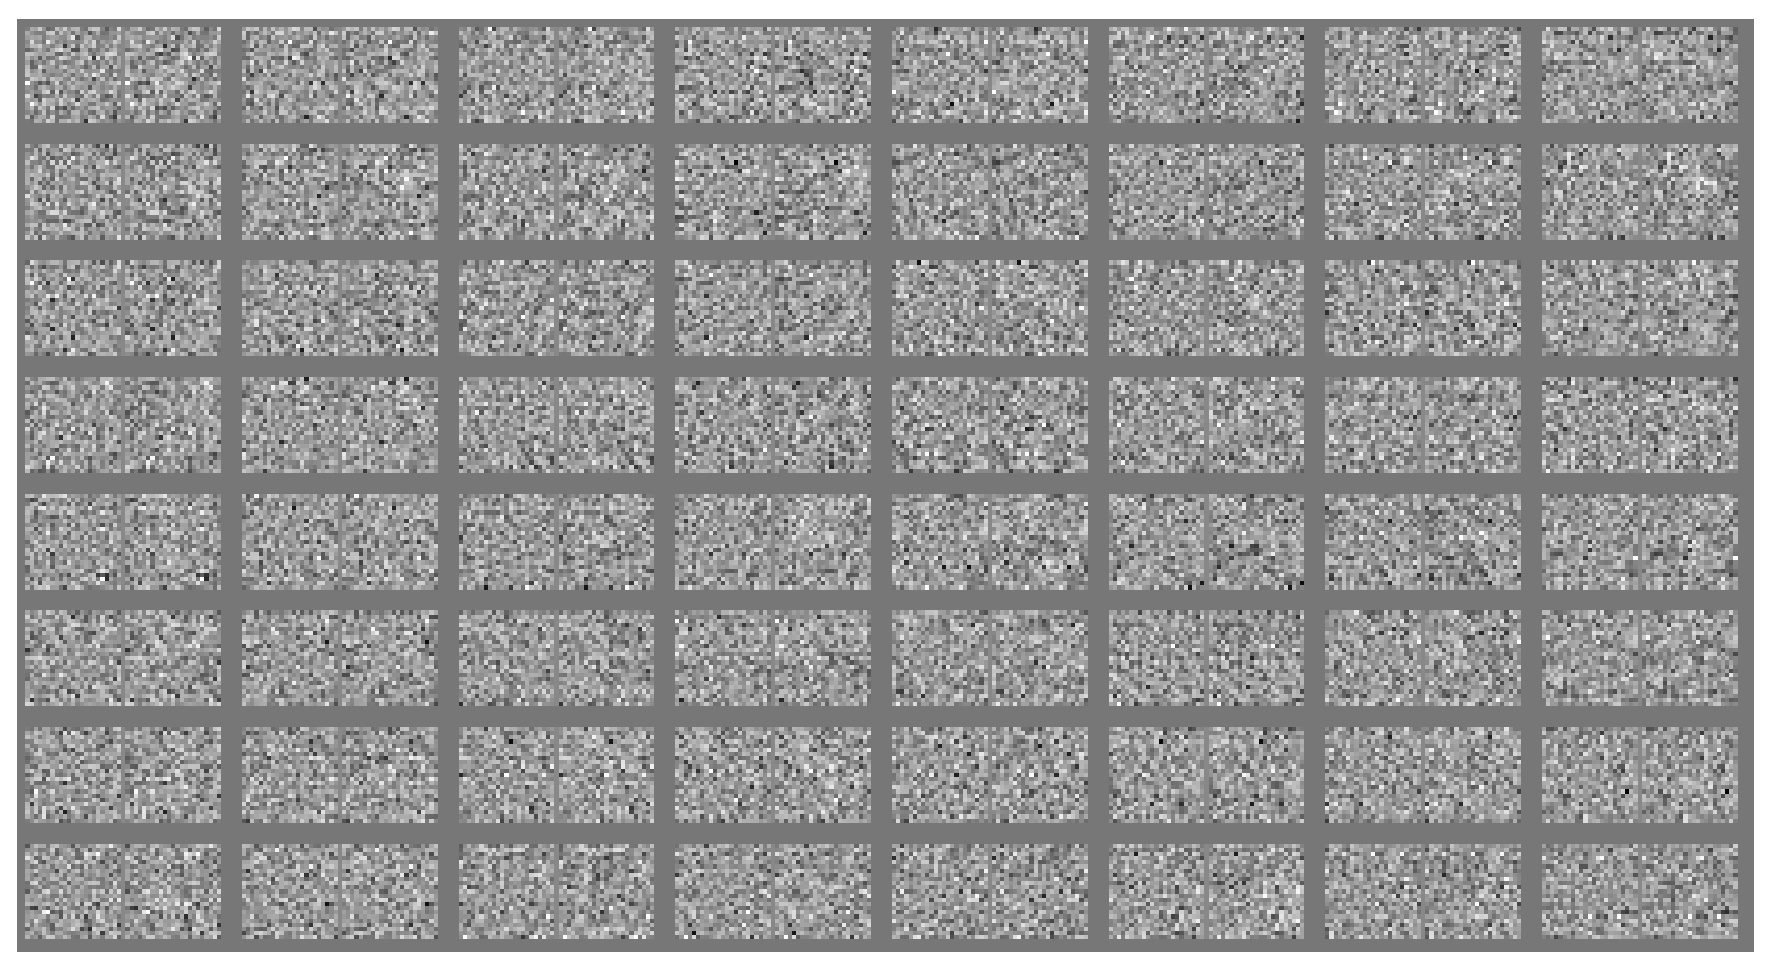
\includegraphics[width=0.9\textwidth]{figures/normal2.eps}} \\
\centering{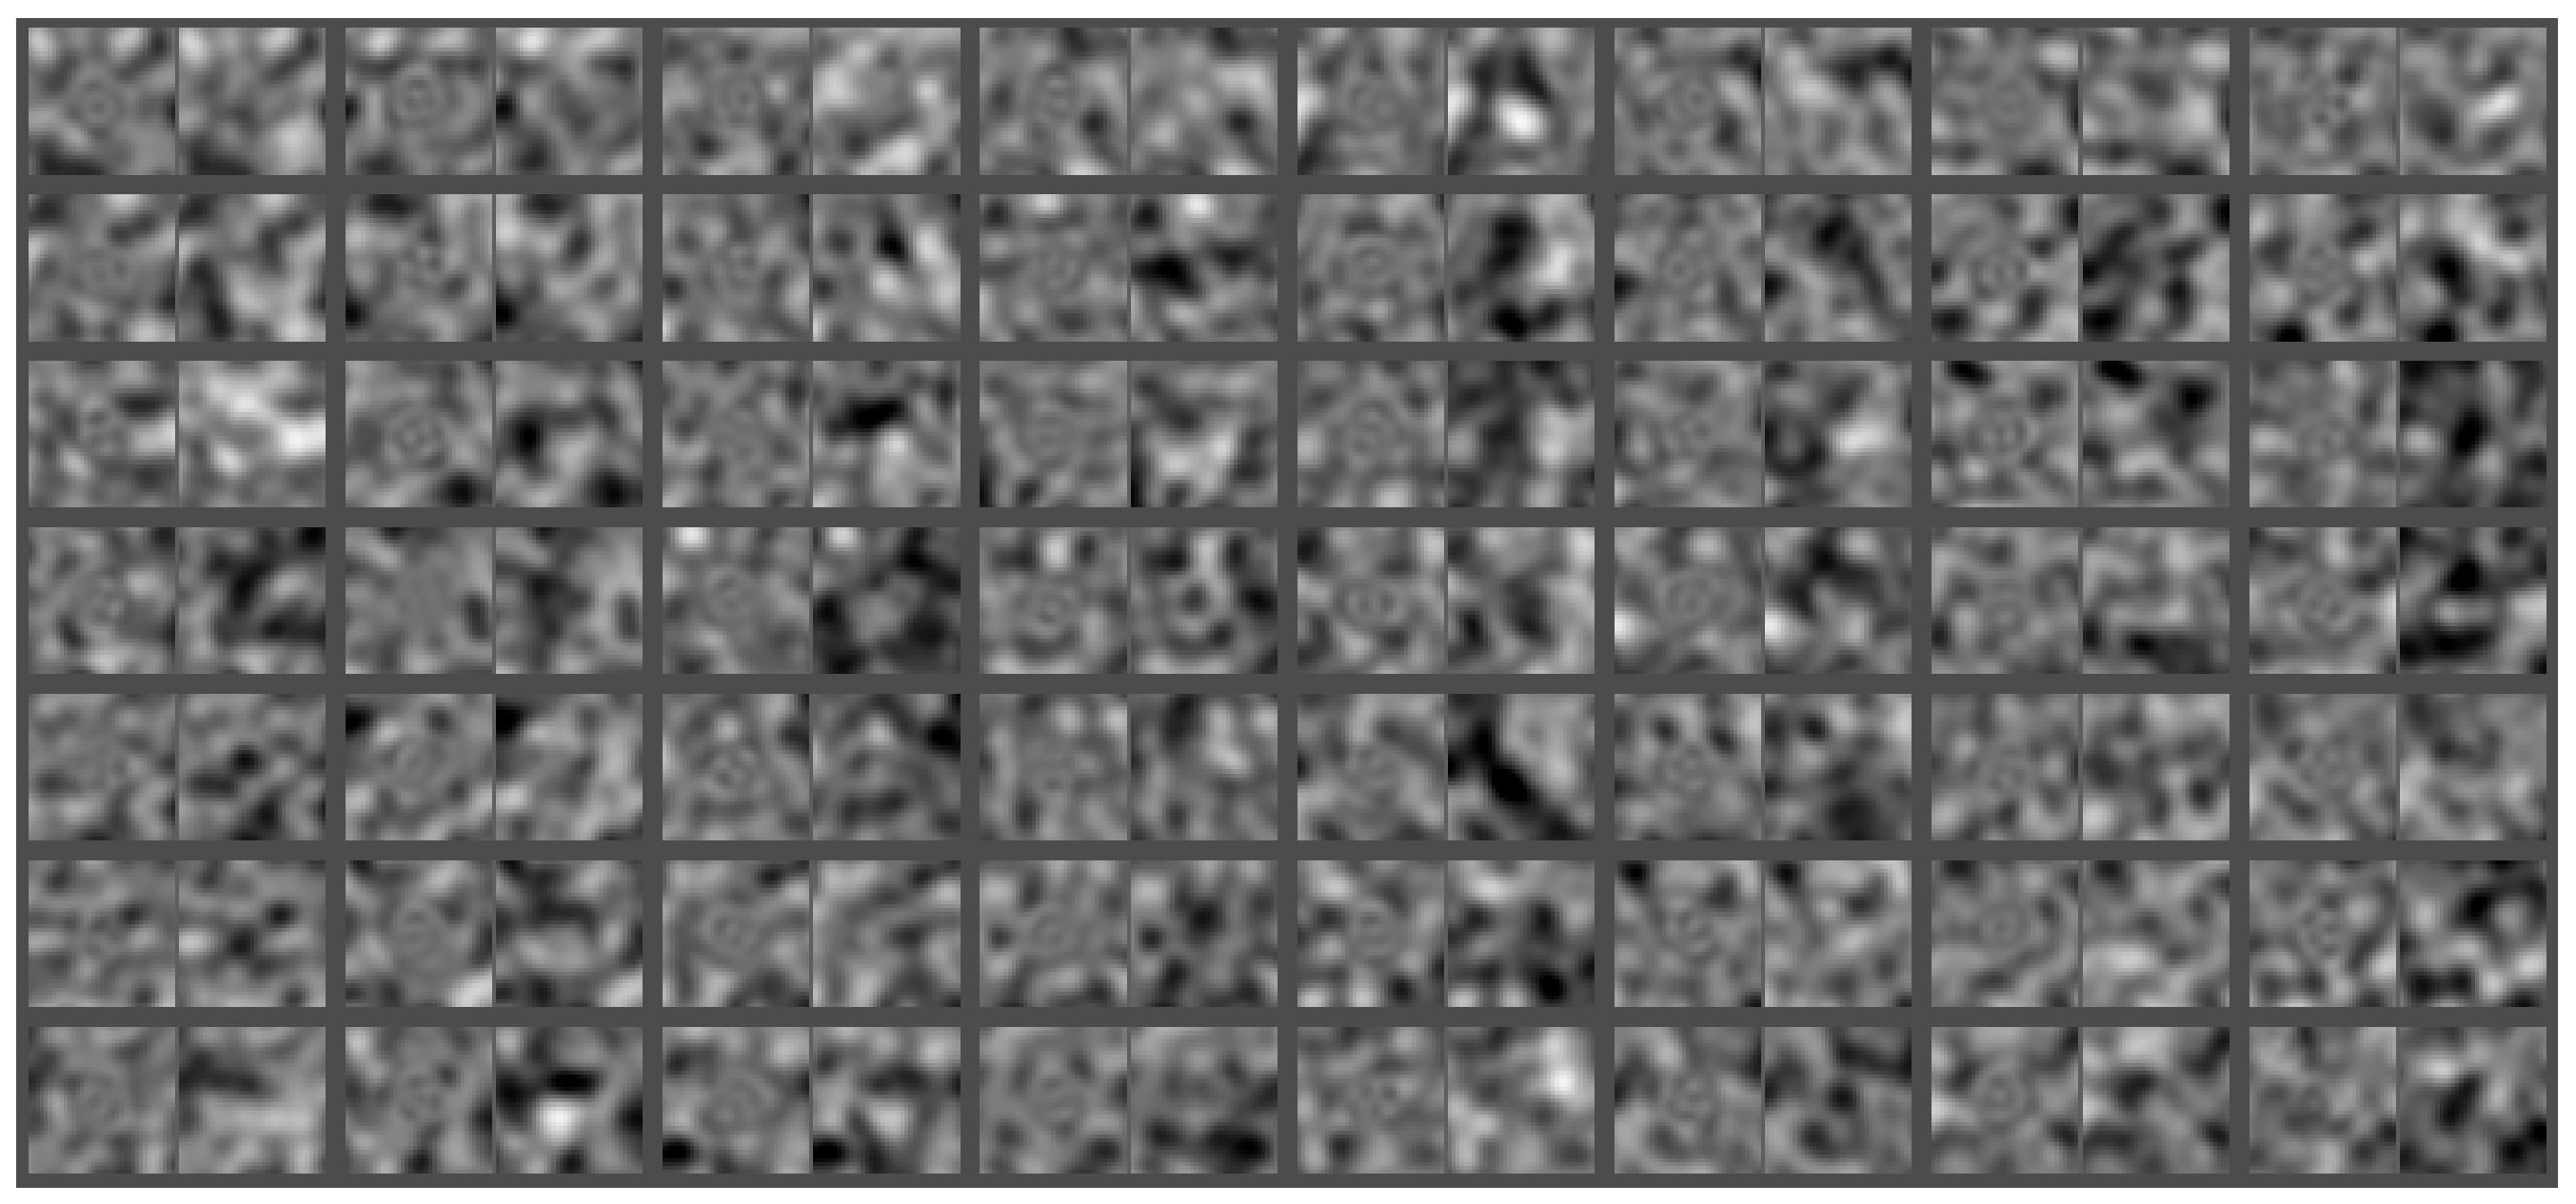
\includegraphics[width=0.9\textwidth]{figures/preconv2.eps}} \\
\end{center}
\caption{Pairs of LOCAL:SPATIAL {\tt KernelCandidate} difference images in the case of
  successful image subtraction, similar to
  Figure~\ref{fig_galleryBad}.  The {\it top} set of data are from
  postfiltered analysis, while the {\it lower} set are from
  prefiltered data.  Note that the noise is smoother in the
  prefiltered data due to correlation with the PSF. }
\label{fig_galleryGood}
\end{figure}

\begin{figure}
\centering{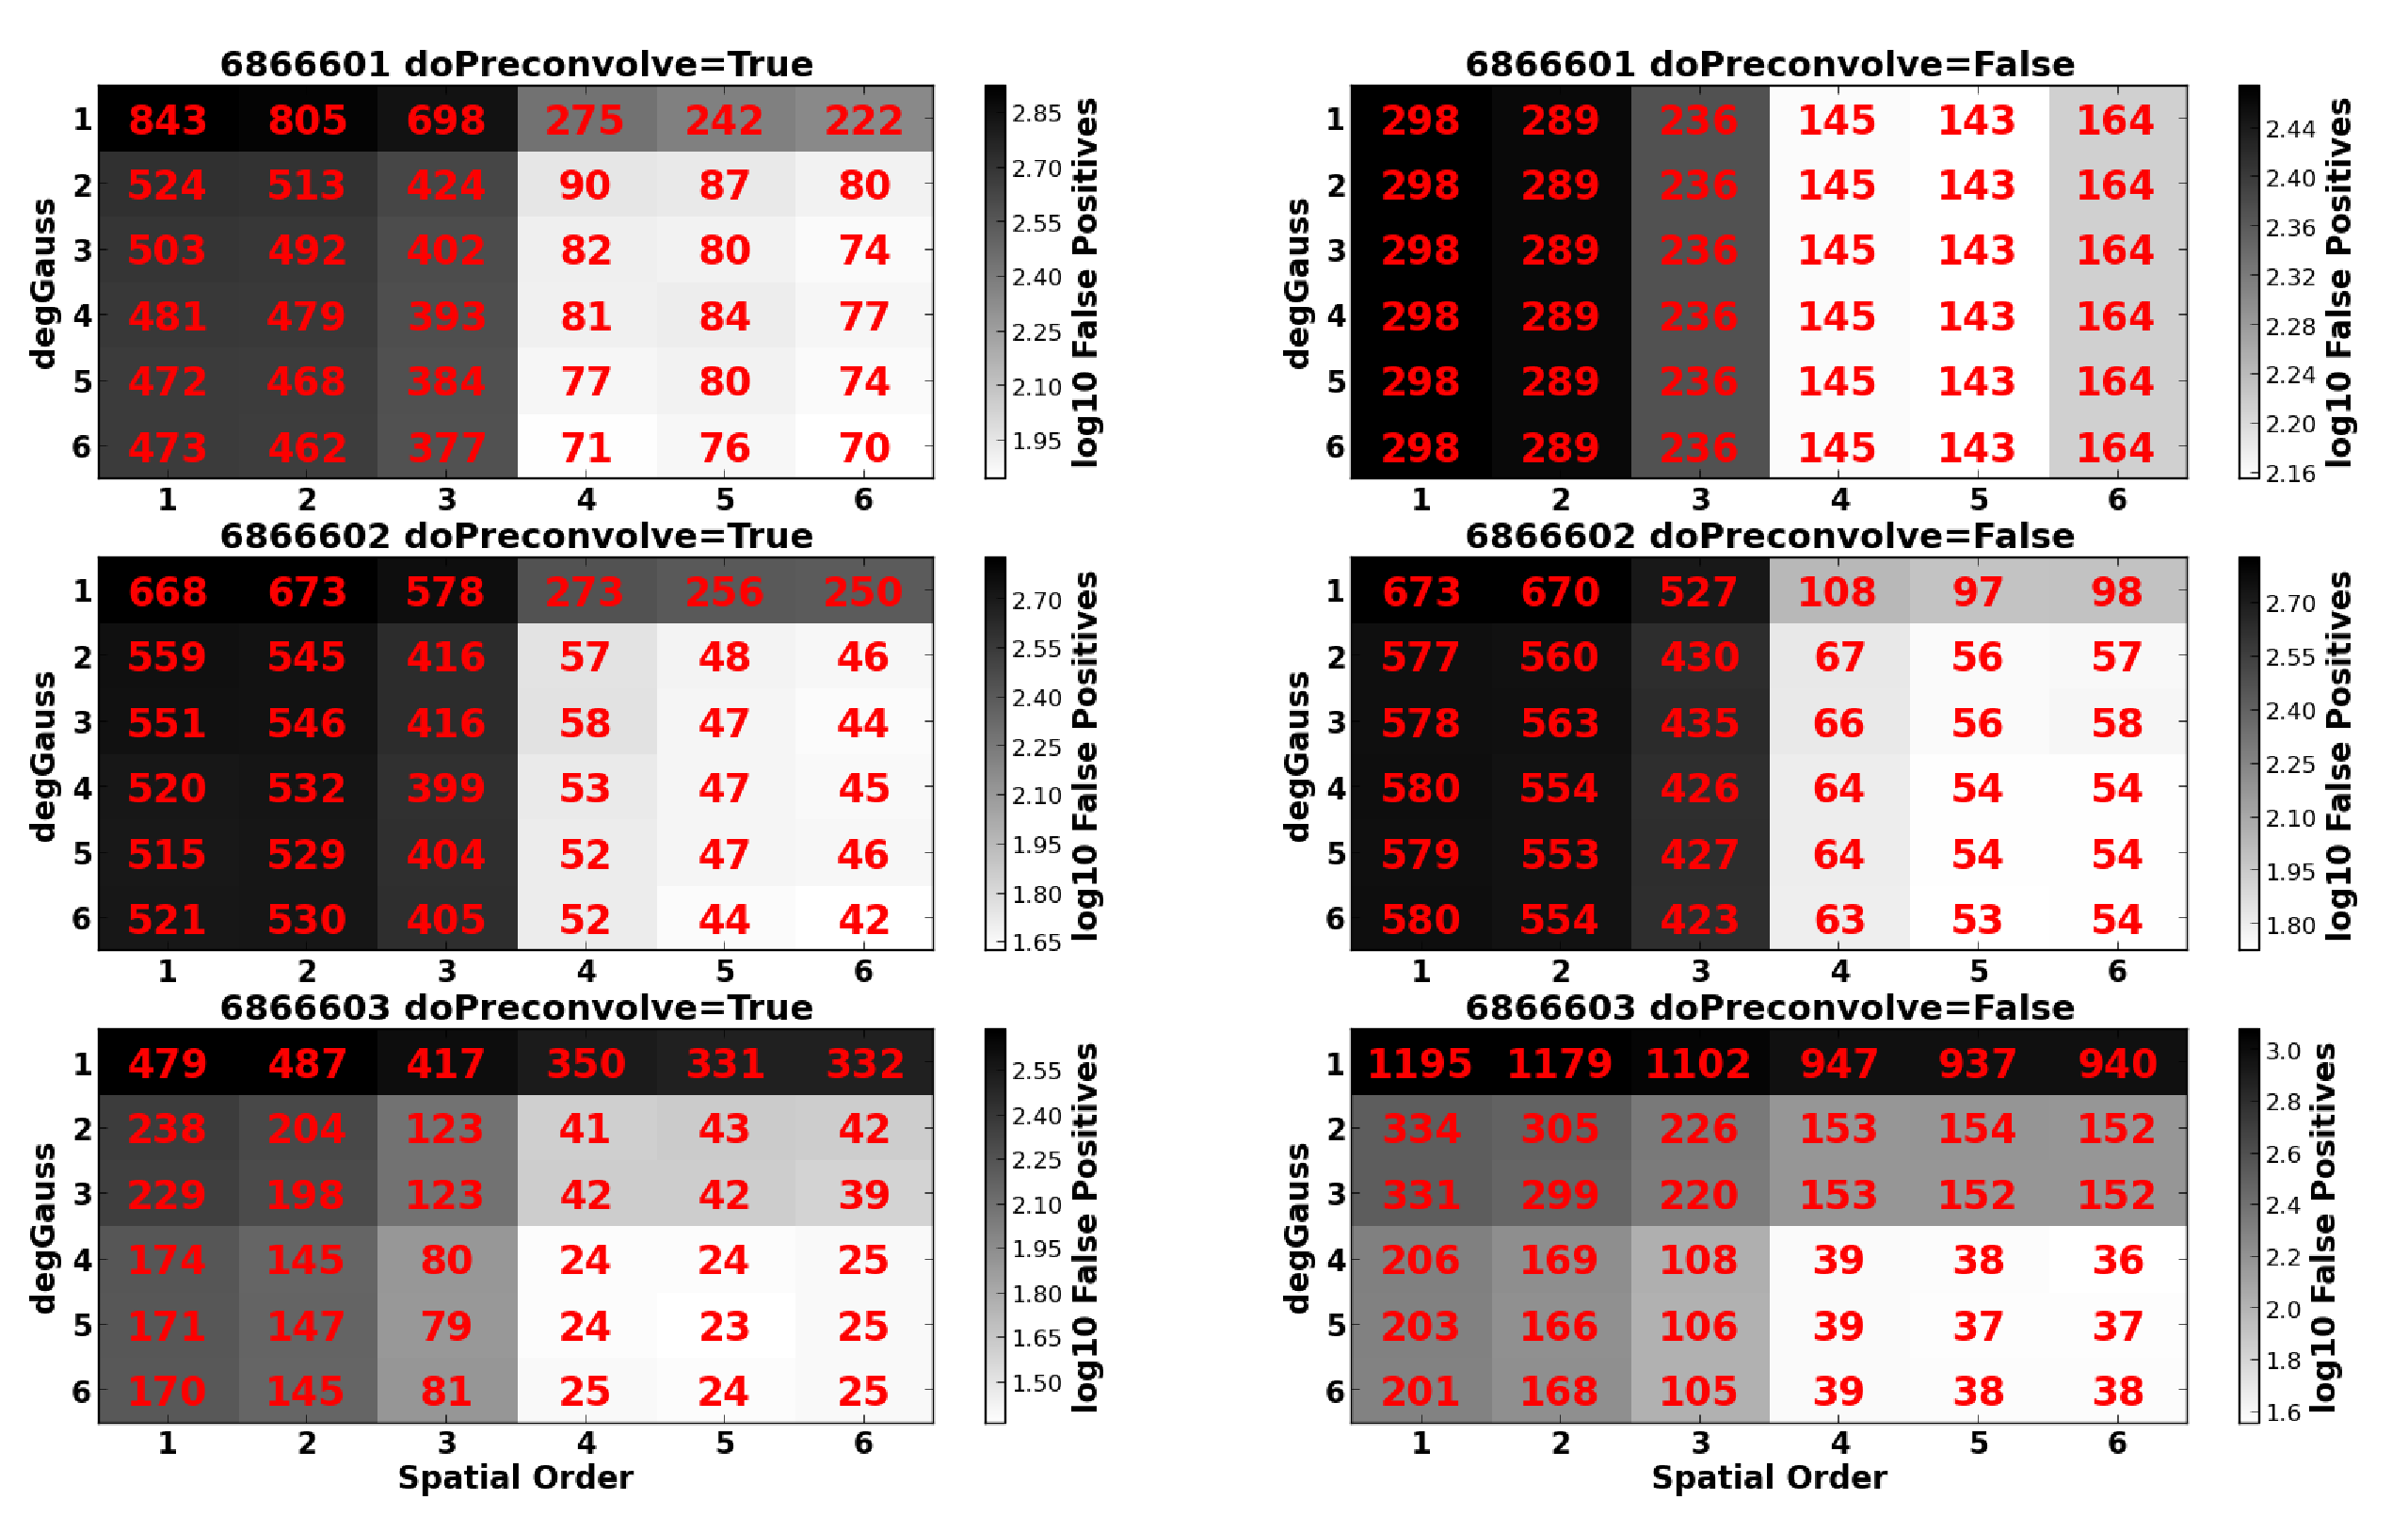
\includegraphics[width=1.0\textwidth]{figures/heatmap10.eps}} \\
\caption{``Heat--map'' detailing the total numbers of 5--sigma false
  positives as a function of two main degrees of freedom: the maximum
  order of basis Laguerre polynomials along the y--axis, and the
  spatial order of the Chebyshev expansion of the spatial model along
  the x--axis.  The {\it left} column shows these results for
  prefiltering, while the {\it right} column shows this for the
  postfiltered analysis.  The best results listed in
  Table~\ref{tab-bestfp10}, with the associated configurations from
  Table~\ref{tab-bestconfig10}, correspond to the minimum in each of the
  subpanels.  }
\label{fp_heatmap}
\end{figure}


\begin{figure}
\centering{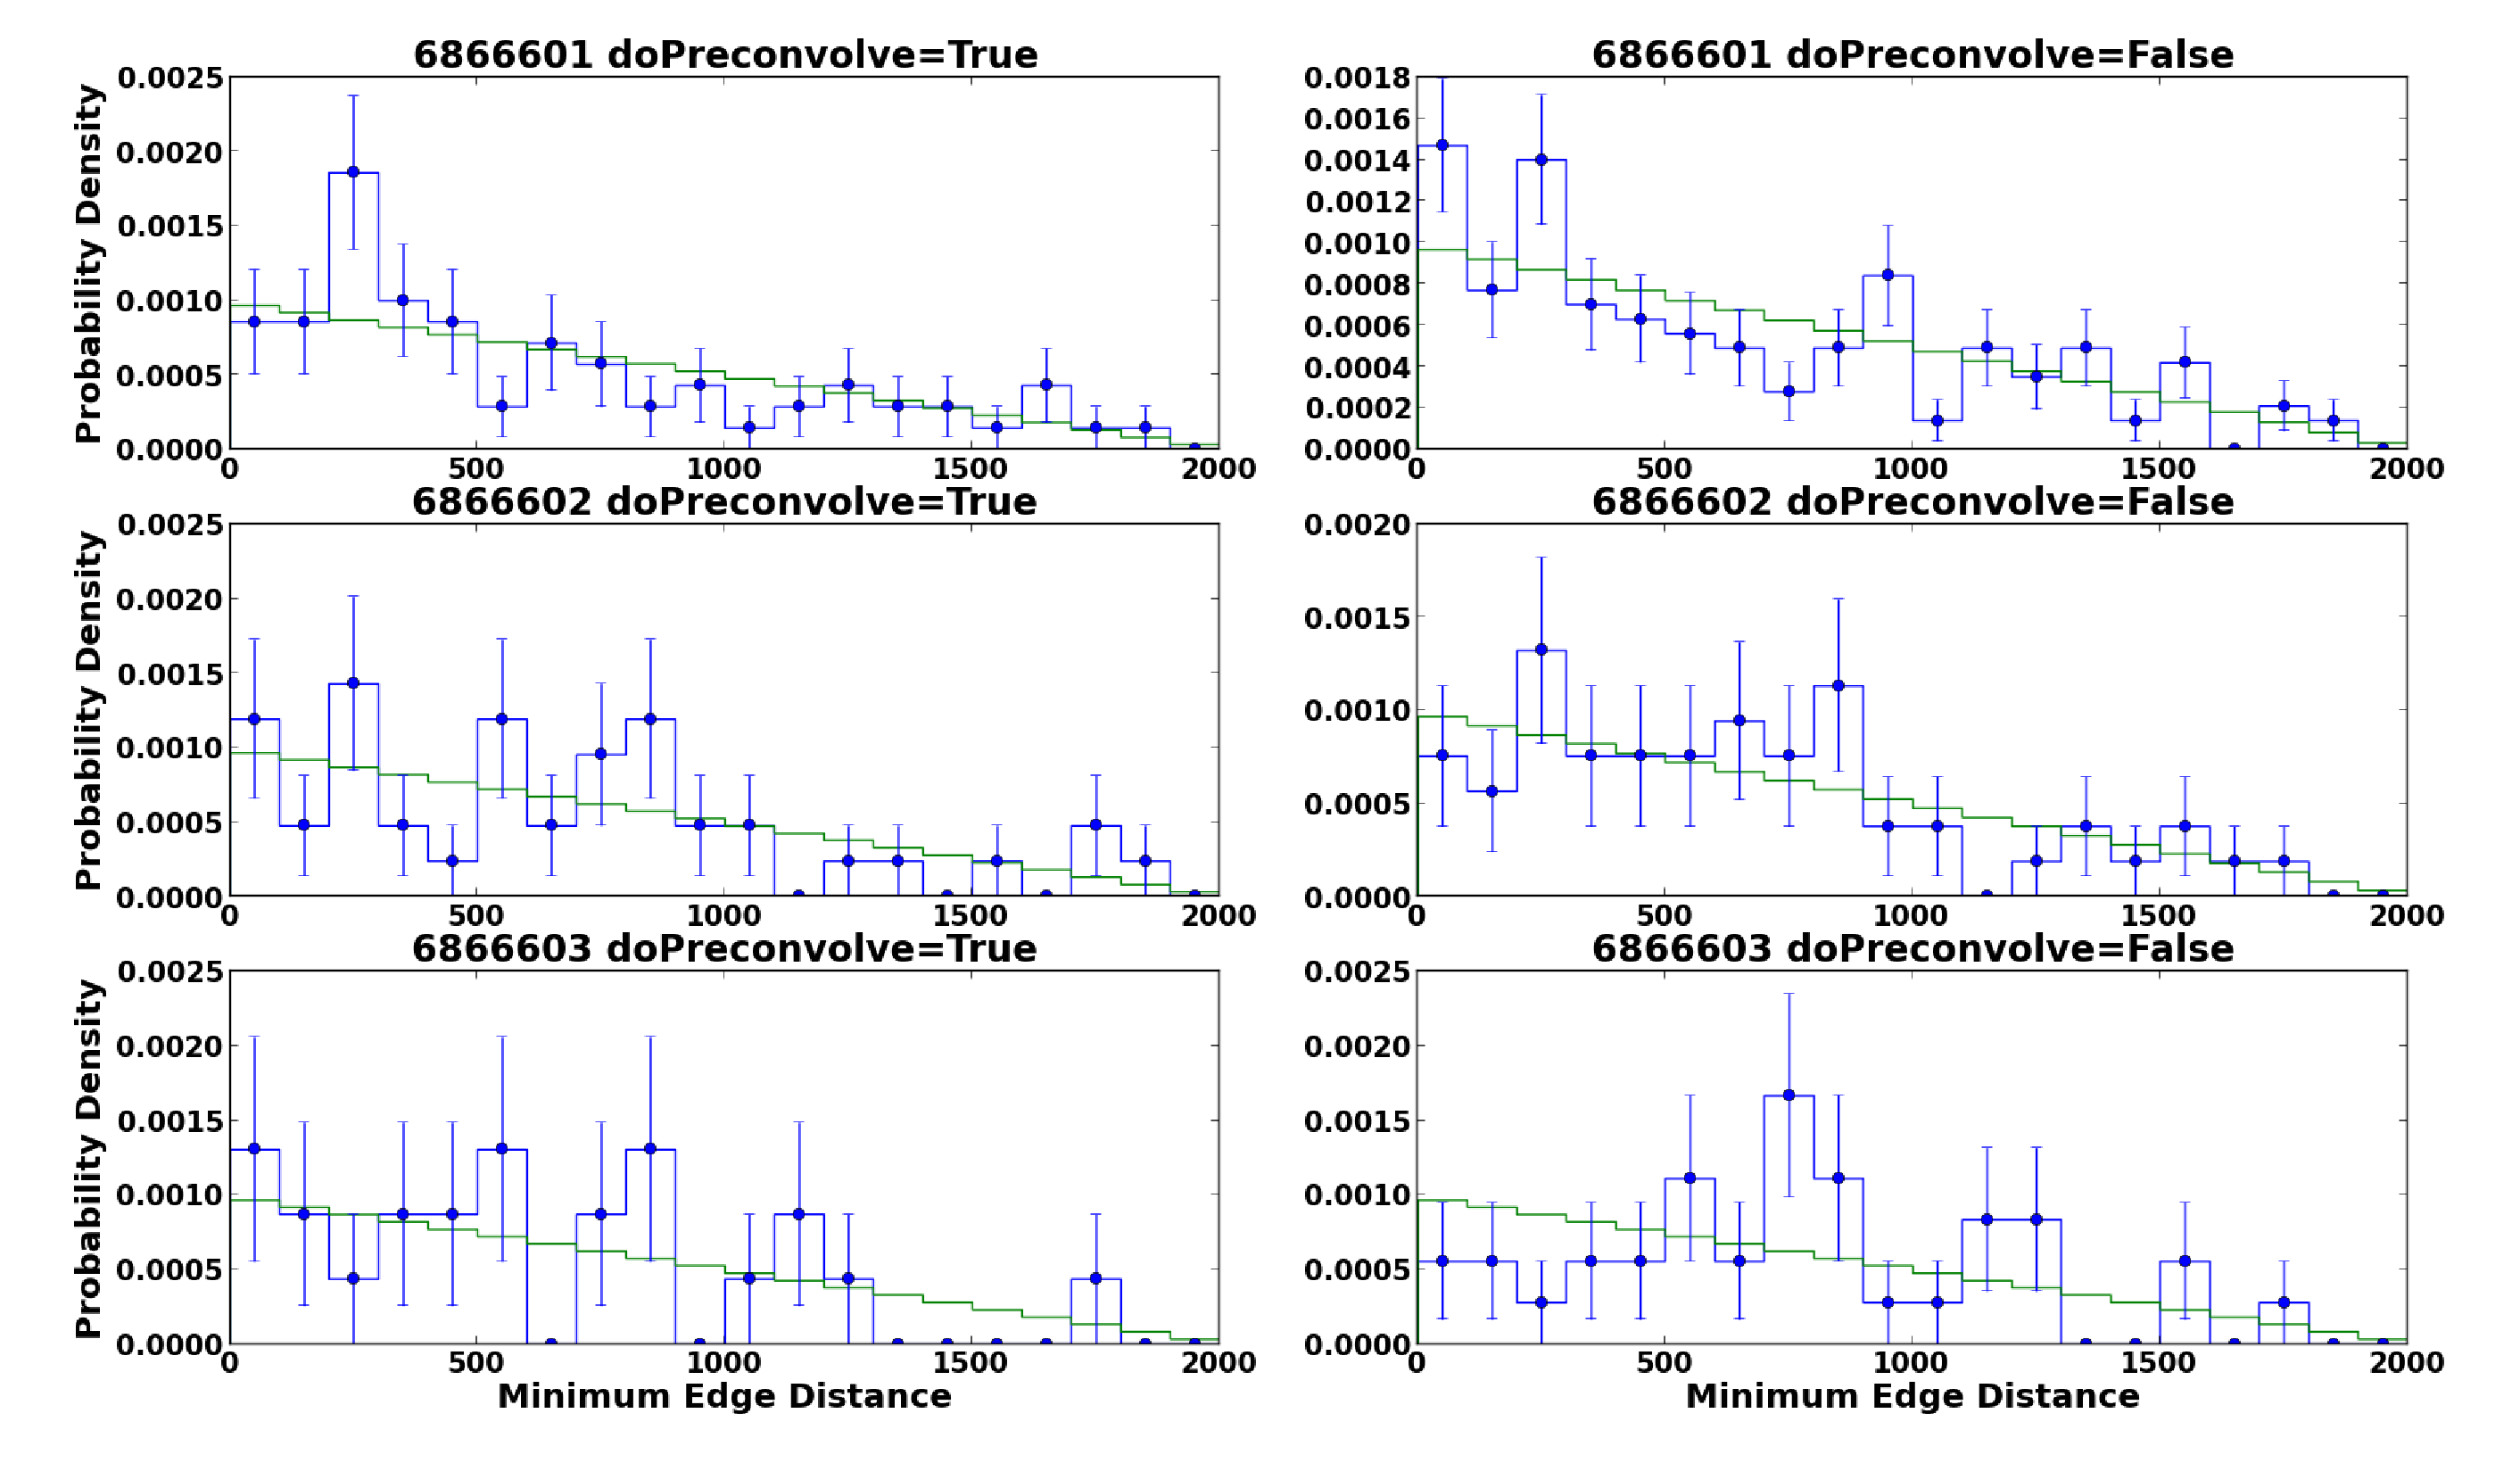
\includegraphics[width=1.0\textwidth]{figures/edge.eps}} \\
\caption{Distribution of false detections as a function of the minimum
  distance from the edge of the sensor.  The {\it green} line shows
  the results from a random distribution of points.  The {\it blue}
  lines show the measured distributions, normalized as a probability
  density ($\sum y~\Delta x = 1$).  Error bars come from the square
  root of the number of points in each bin. }
\label{edgedist}
\end{figure}

\begin{figure}
  \centering 
  \subfloat[][0.6$^{\prime\prime}$ FWHM]{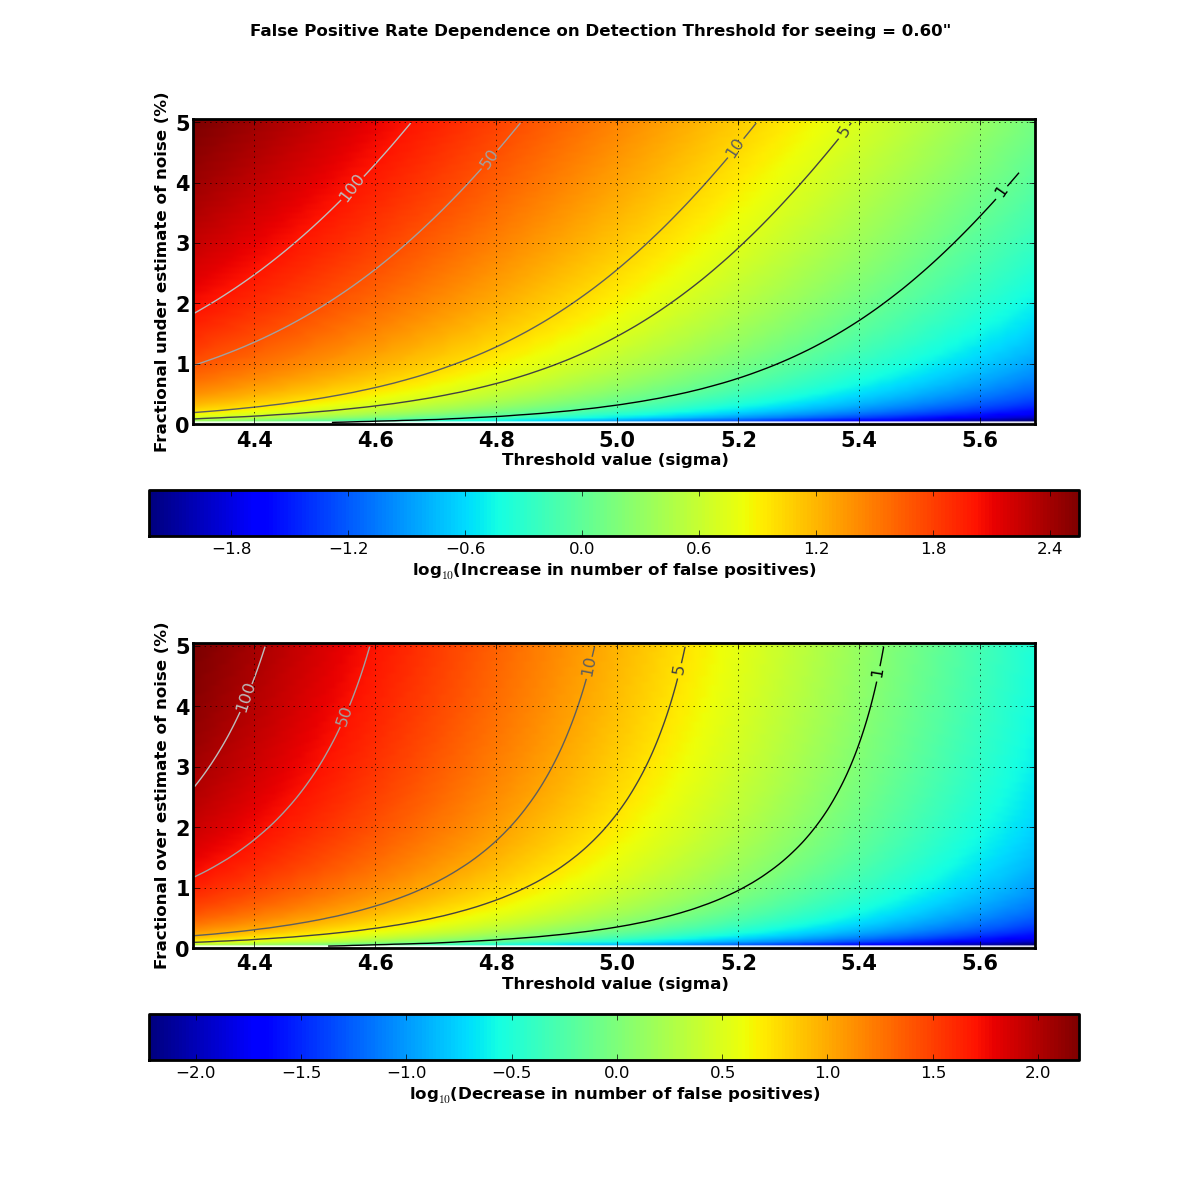
\includegraphics[width=1.0\textwidth]{figures/dfp_v_sigma0.60.eps}}
  \caption[]{ We plot here the effect on the number of false positives
    as a function of detection threshold and noise misestimate.  The
    panels on these 3 pages are for three values of seeing.  In each panel the
    top pane shows what happens when the noise is under-estimated and
    the bottom shows what happens to the false positive rate when the
    noise is over-estimated.  In all cases the counts are for the
    total number of false positives in a single 4000x4072 pixel random
    Gaussian field.
    }
  \label{fig-fpthresh}
\end{figure}
\clearpage
\begin{figure}
  \ContinuedFloat 
  \centering 
  \subfloat[][0.88$^{\prime\prime}$ FWHM]{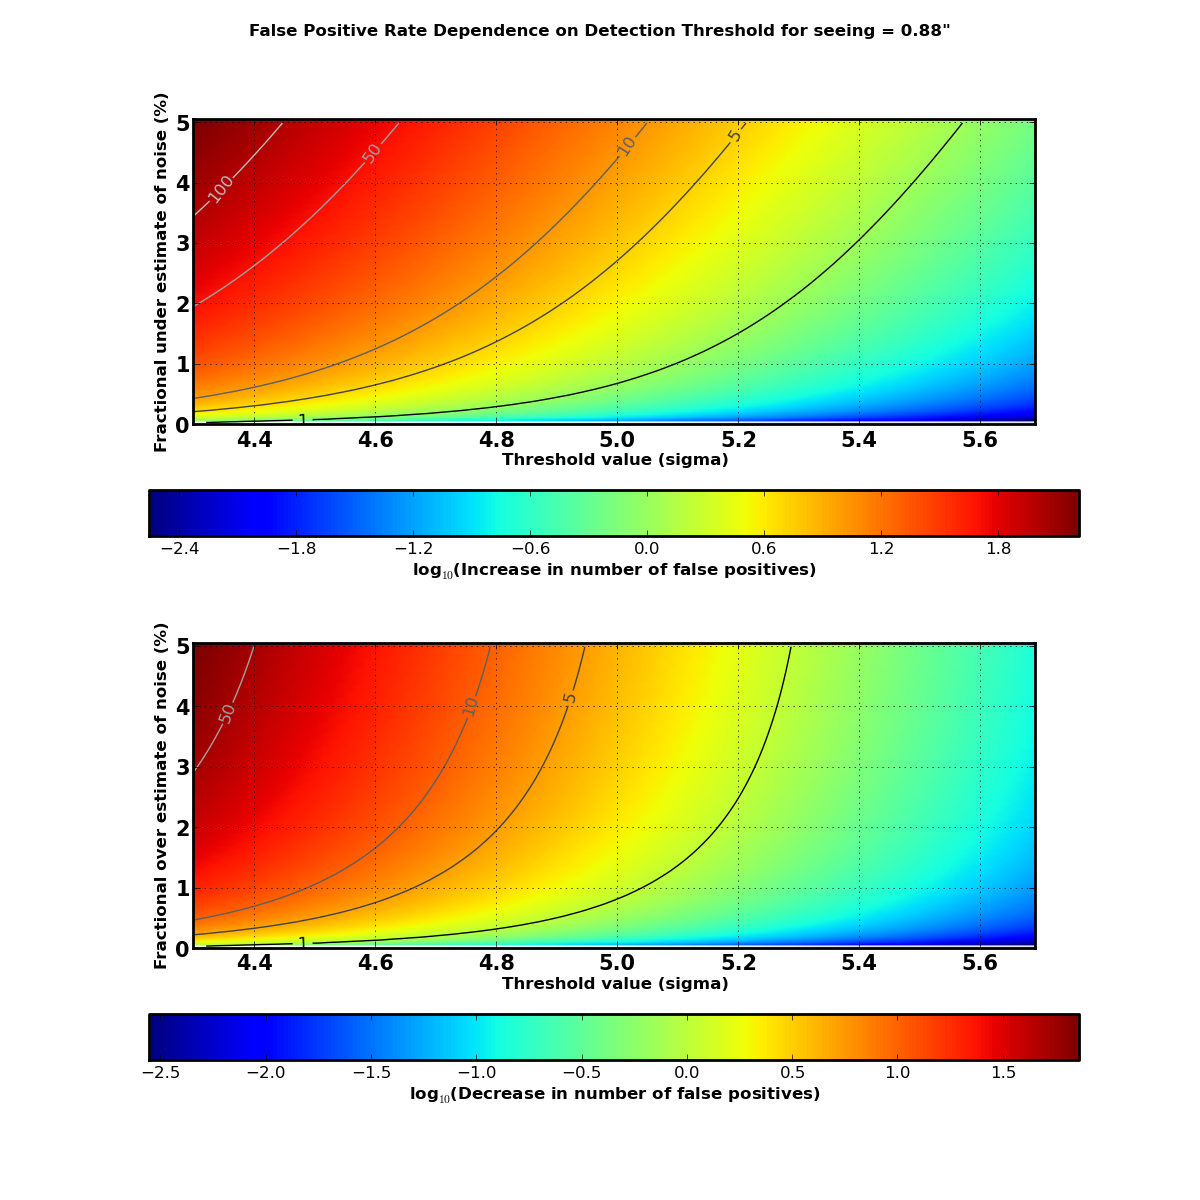
\includegraphics[width=1.0\textwidth]{figures/dfp_v_sigma0.88.eps}}
\end{figure} 
\clearpage
\begin{figure}
  \ContinuedFloat 
  \centering 
  \subfloat[][1.2$^{\prime\prime}$ FWHM]{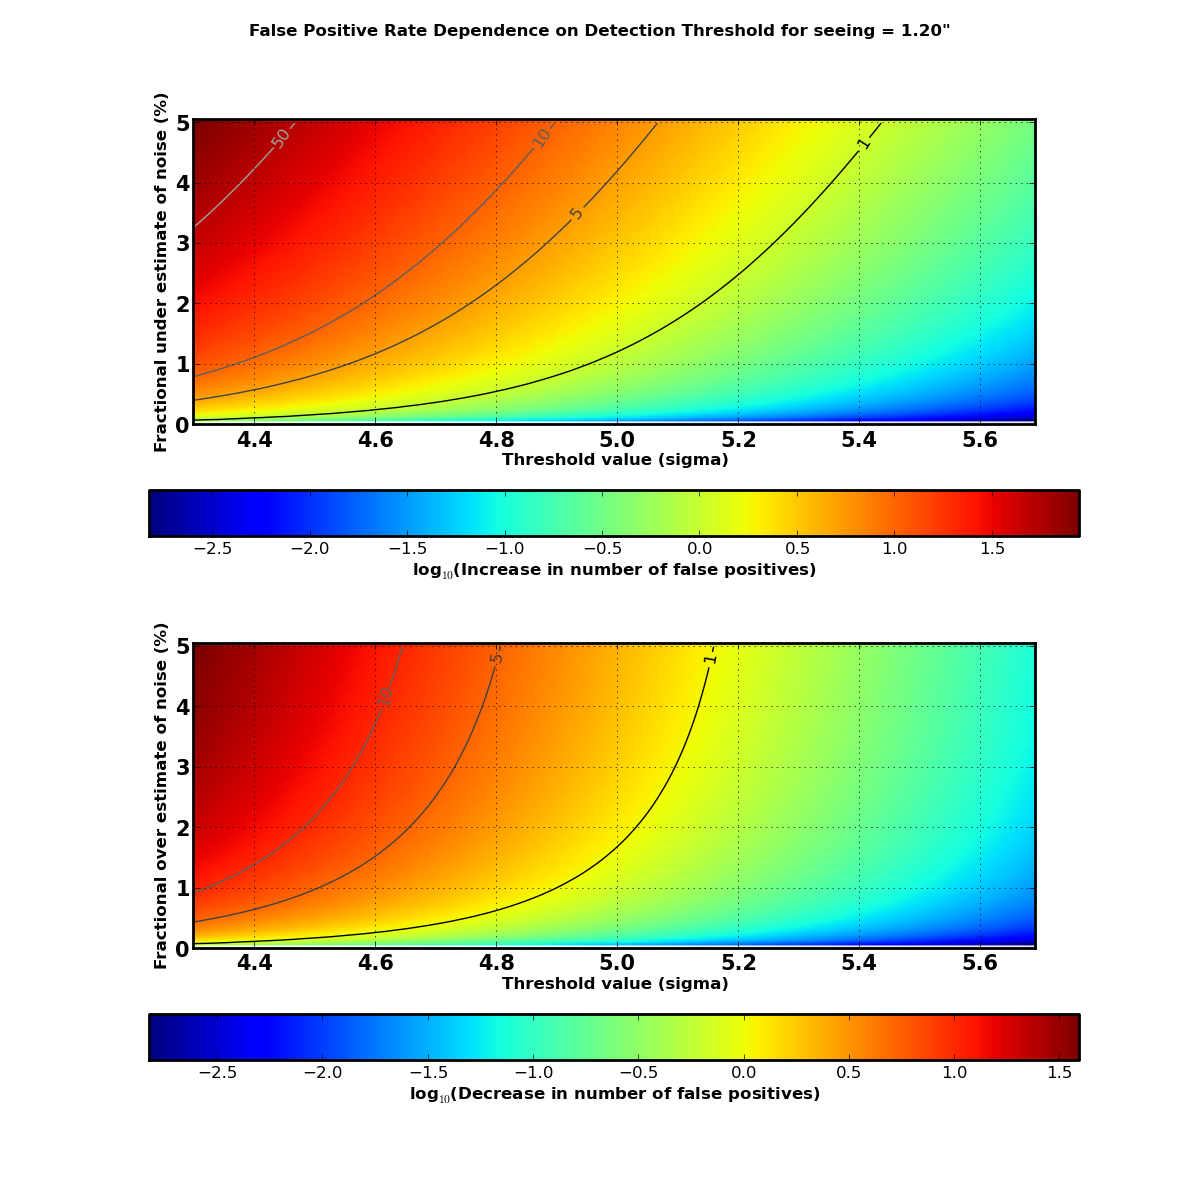
\includegraphics[width=1.0\textwidth]{figures/dfp_v_sigma1.20.eps}}
\end{figure} 

\begin{figure}
\centering
\centering{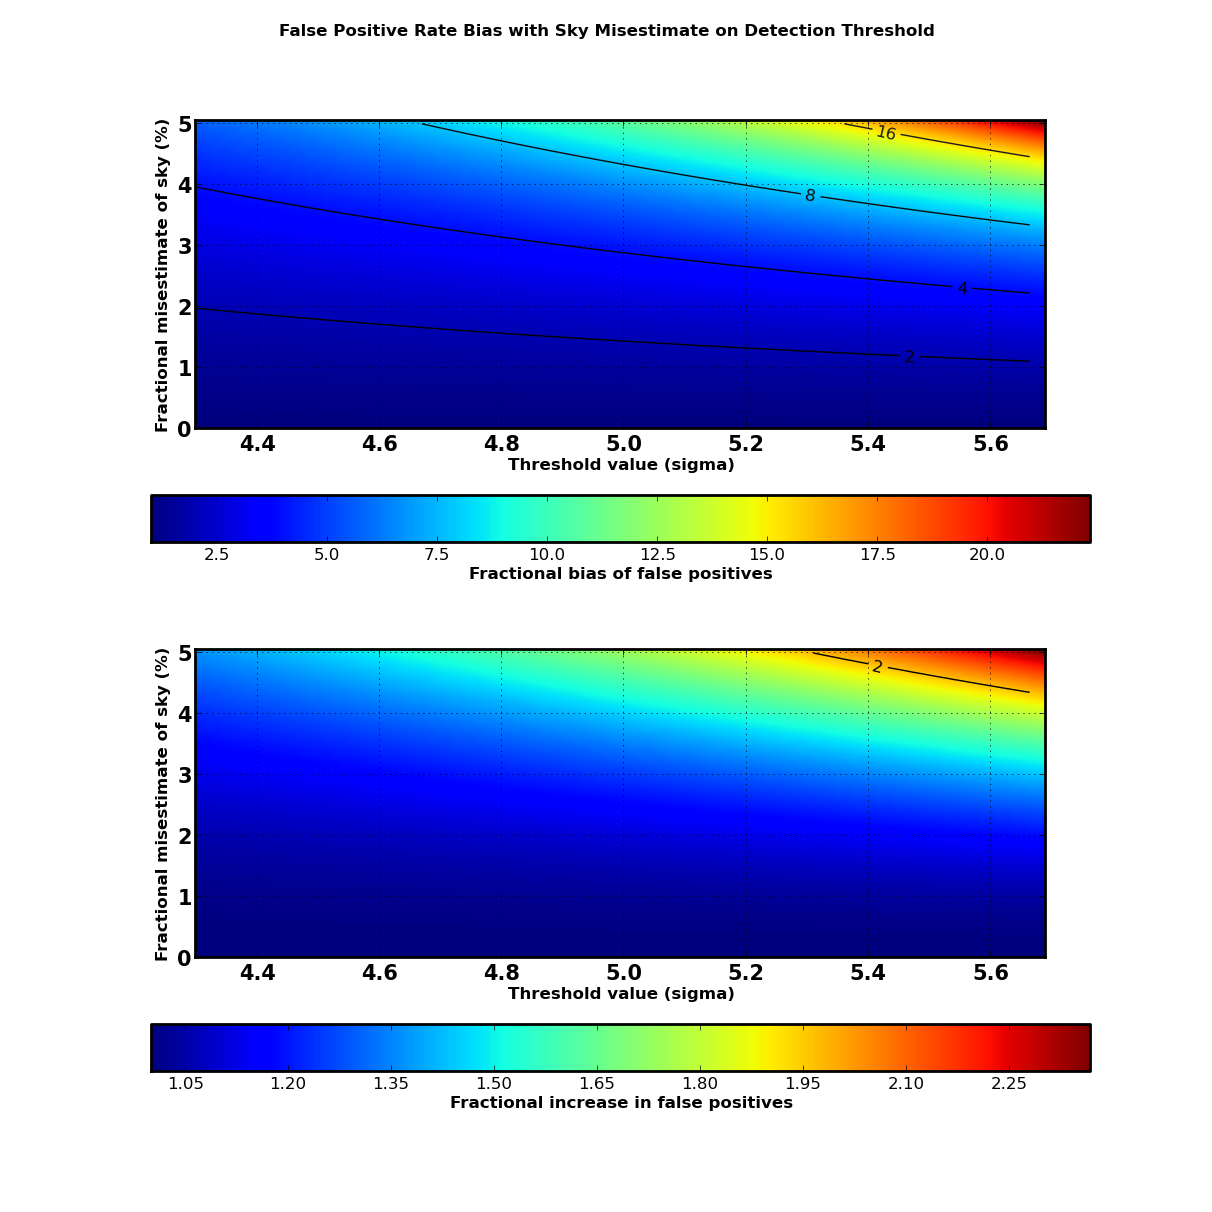
\includegraphics[width=1.0\textwidth]{figures/fp_v_dsky.eps}}
\caption{
Misestimation of the sky value has an effect on both the number of false positives and relative abundance of positive false positives to negative false positives.
The top pane of this figure shows the relative number of +ve/-ve (-ve/+ve) if the sky background is under (over) subtracted at a particular fractional level.  The 
bottom panel shows how the total number of false positives changes for the same misestimation.  This is not a strong function of the seeing, so only the best
seeing example is shown.
}
\label{fig-skythresh}
\end{figure}

\begin{figure}
\centering{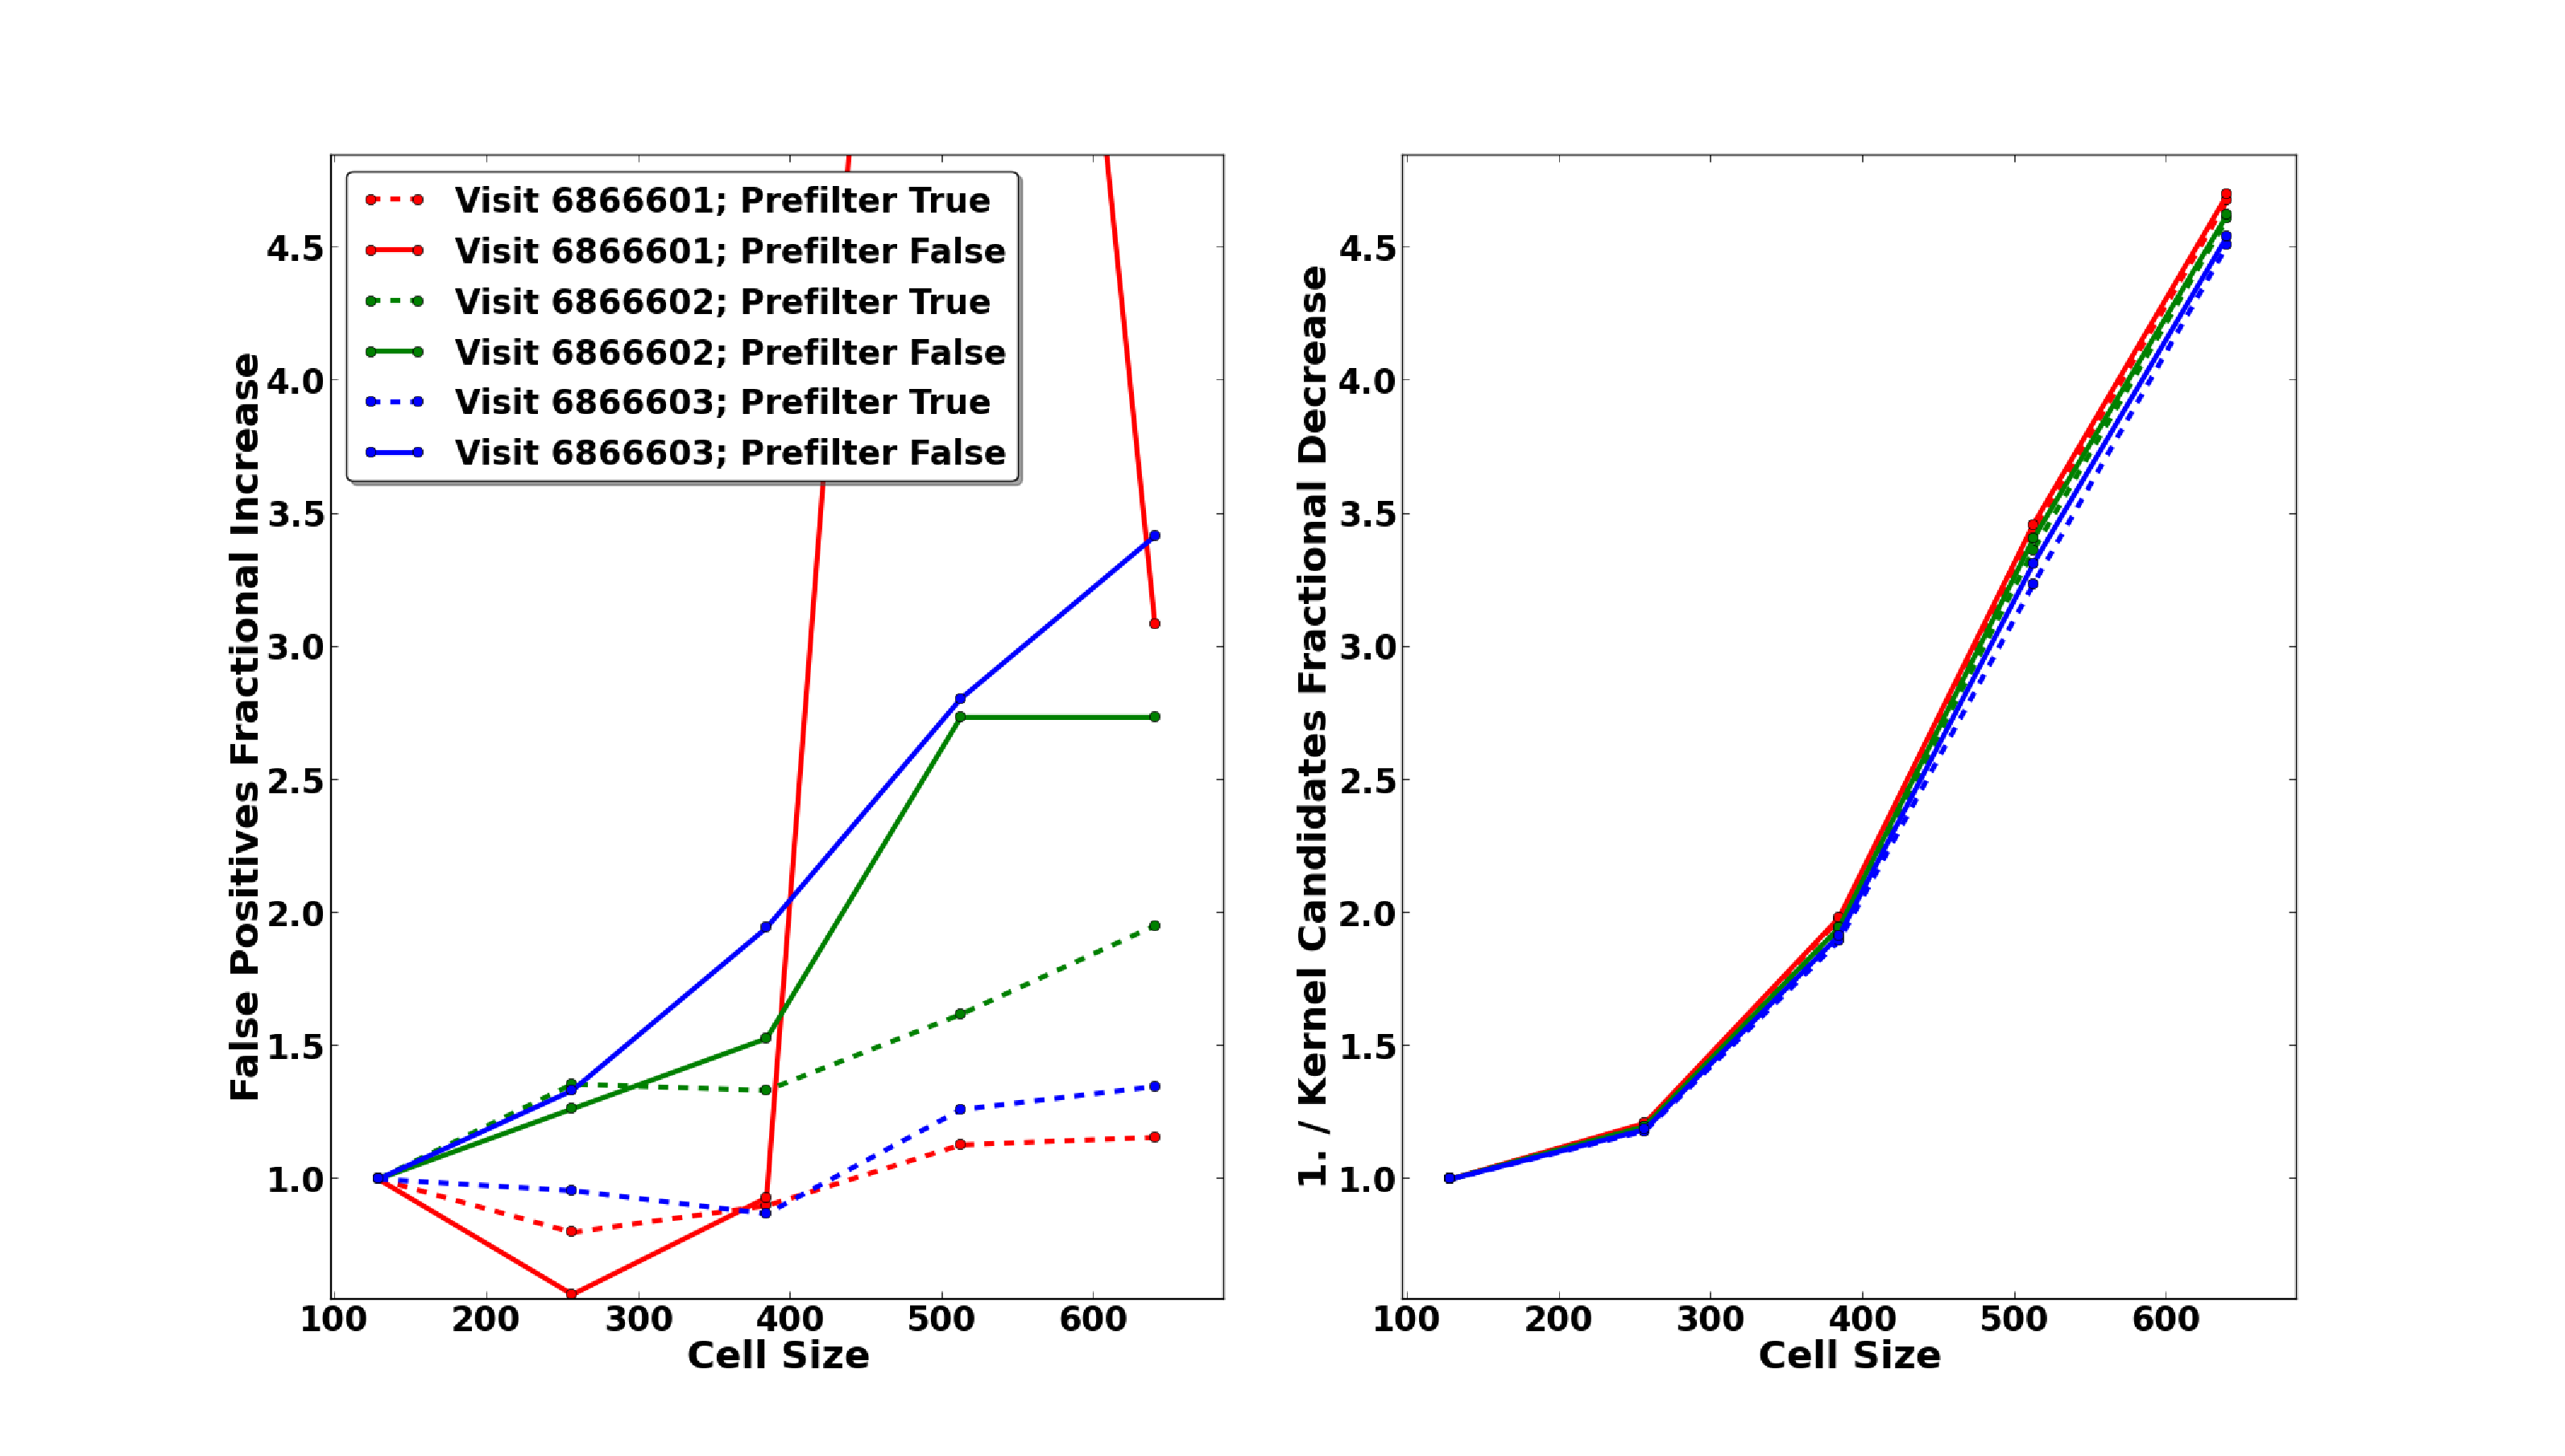
\includegraphics[width=1.0\textwidth]{figures/cellsize.eps}} \\
\caption{We show the number of false detections ({\it left}) and {\tt
    KernelCandidates} used in the spatial kernel fit ({\it right}) as
  a function of {\tt SpatialCell} size.  Increasing the cell size,
  while keep all other things equal, effectively decreases the number
  of constraints on the spatial model.  As shown on the left, the
  prefiltered data ({\it dashed} lines) have a less strong dependence
  on the number of constraints compared to the postfiltered data ({\it
    solid} lines).  The prefiltered data show essentially similar
  quality when using 300 vs. 600 {\tt KernelCandidates}, while in the
  postfiltered data the number of false positives increases by nearly
  a factor of 2 (from cellsize 128 to 384).  }
\label{cellsize}
\end{figure}

\begin{figure}
\centering{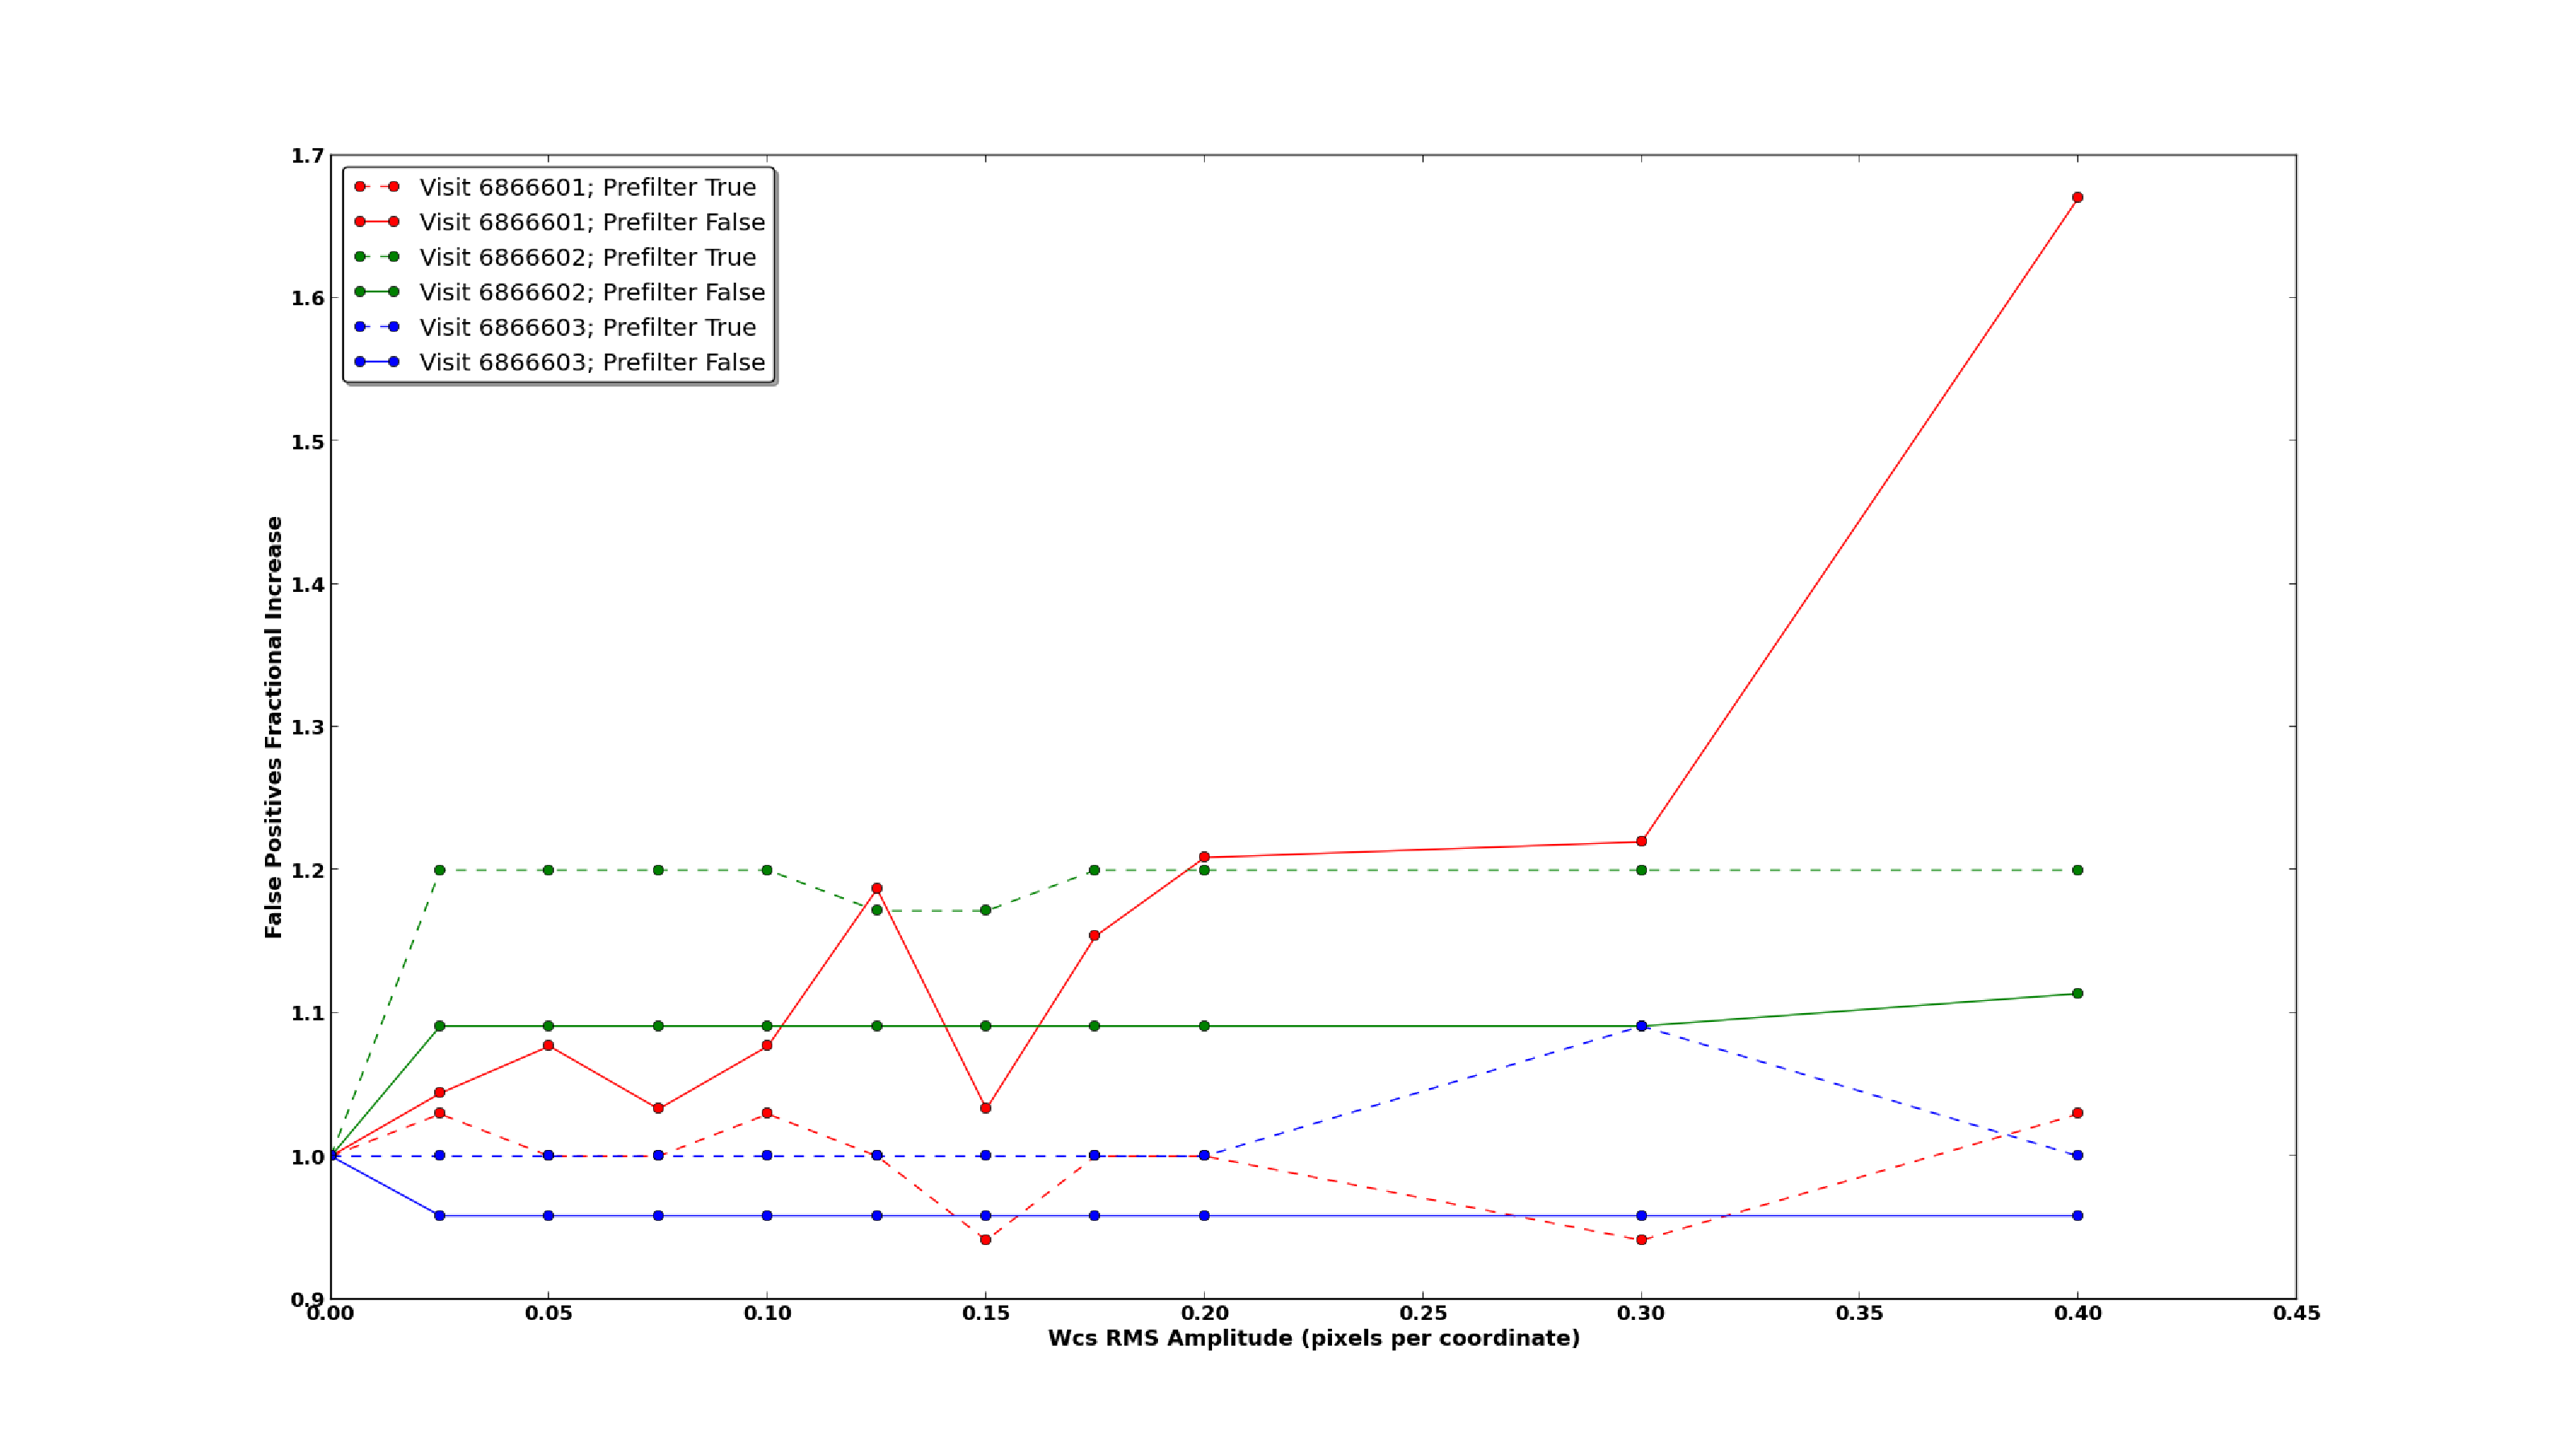
\includegraphics[width=1.0\textwidth]{figures/wcs_rms.eps}} \\
\caption{Fractional increase in false detections as a function of the
  amplitude of random astrometric offsets added to the coordinates of
  sources before image-to-image registration.  The {\it red}, {\it
    green}, and {\it blue} lines correspond to visits v6866601,
  v6866602, and v6866603 respectively, while the {\it dashed} and {\it
    solid} lines correspond to prefiltering and postfiltering,
  respectively.}
\label{wcsrms}
\end{figure}

\begin{figure}
\centering{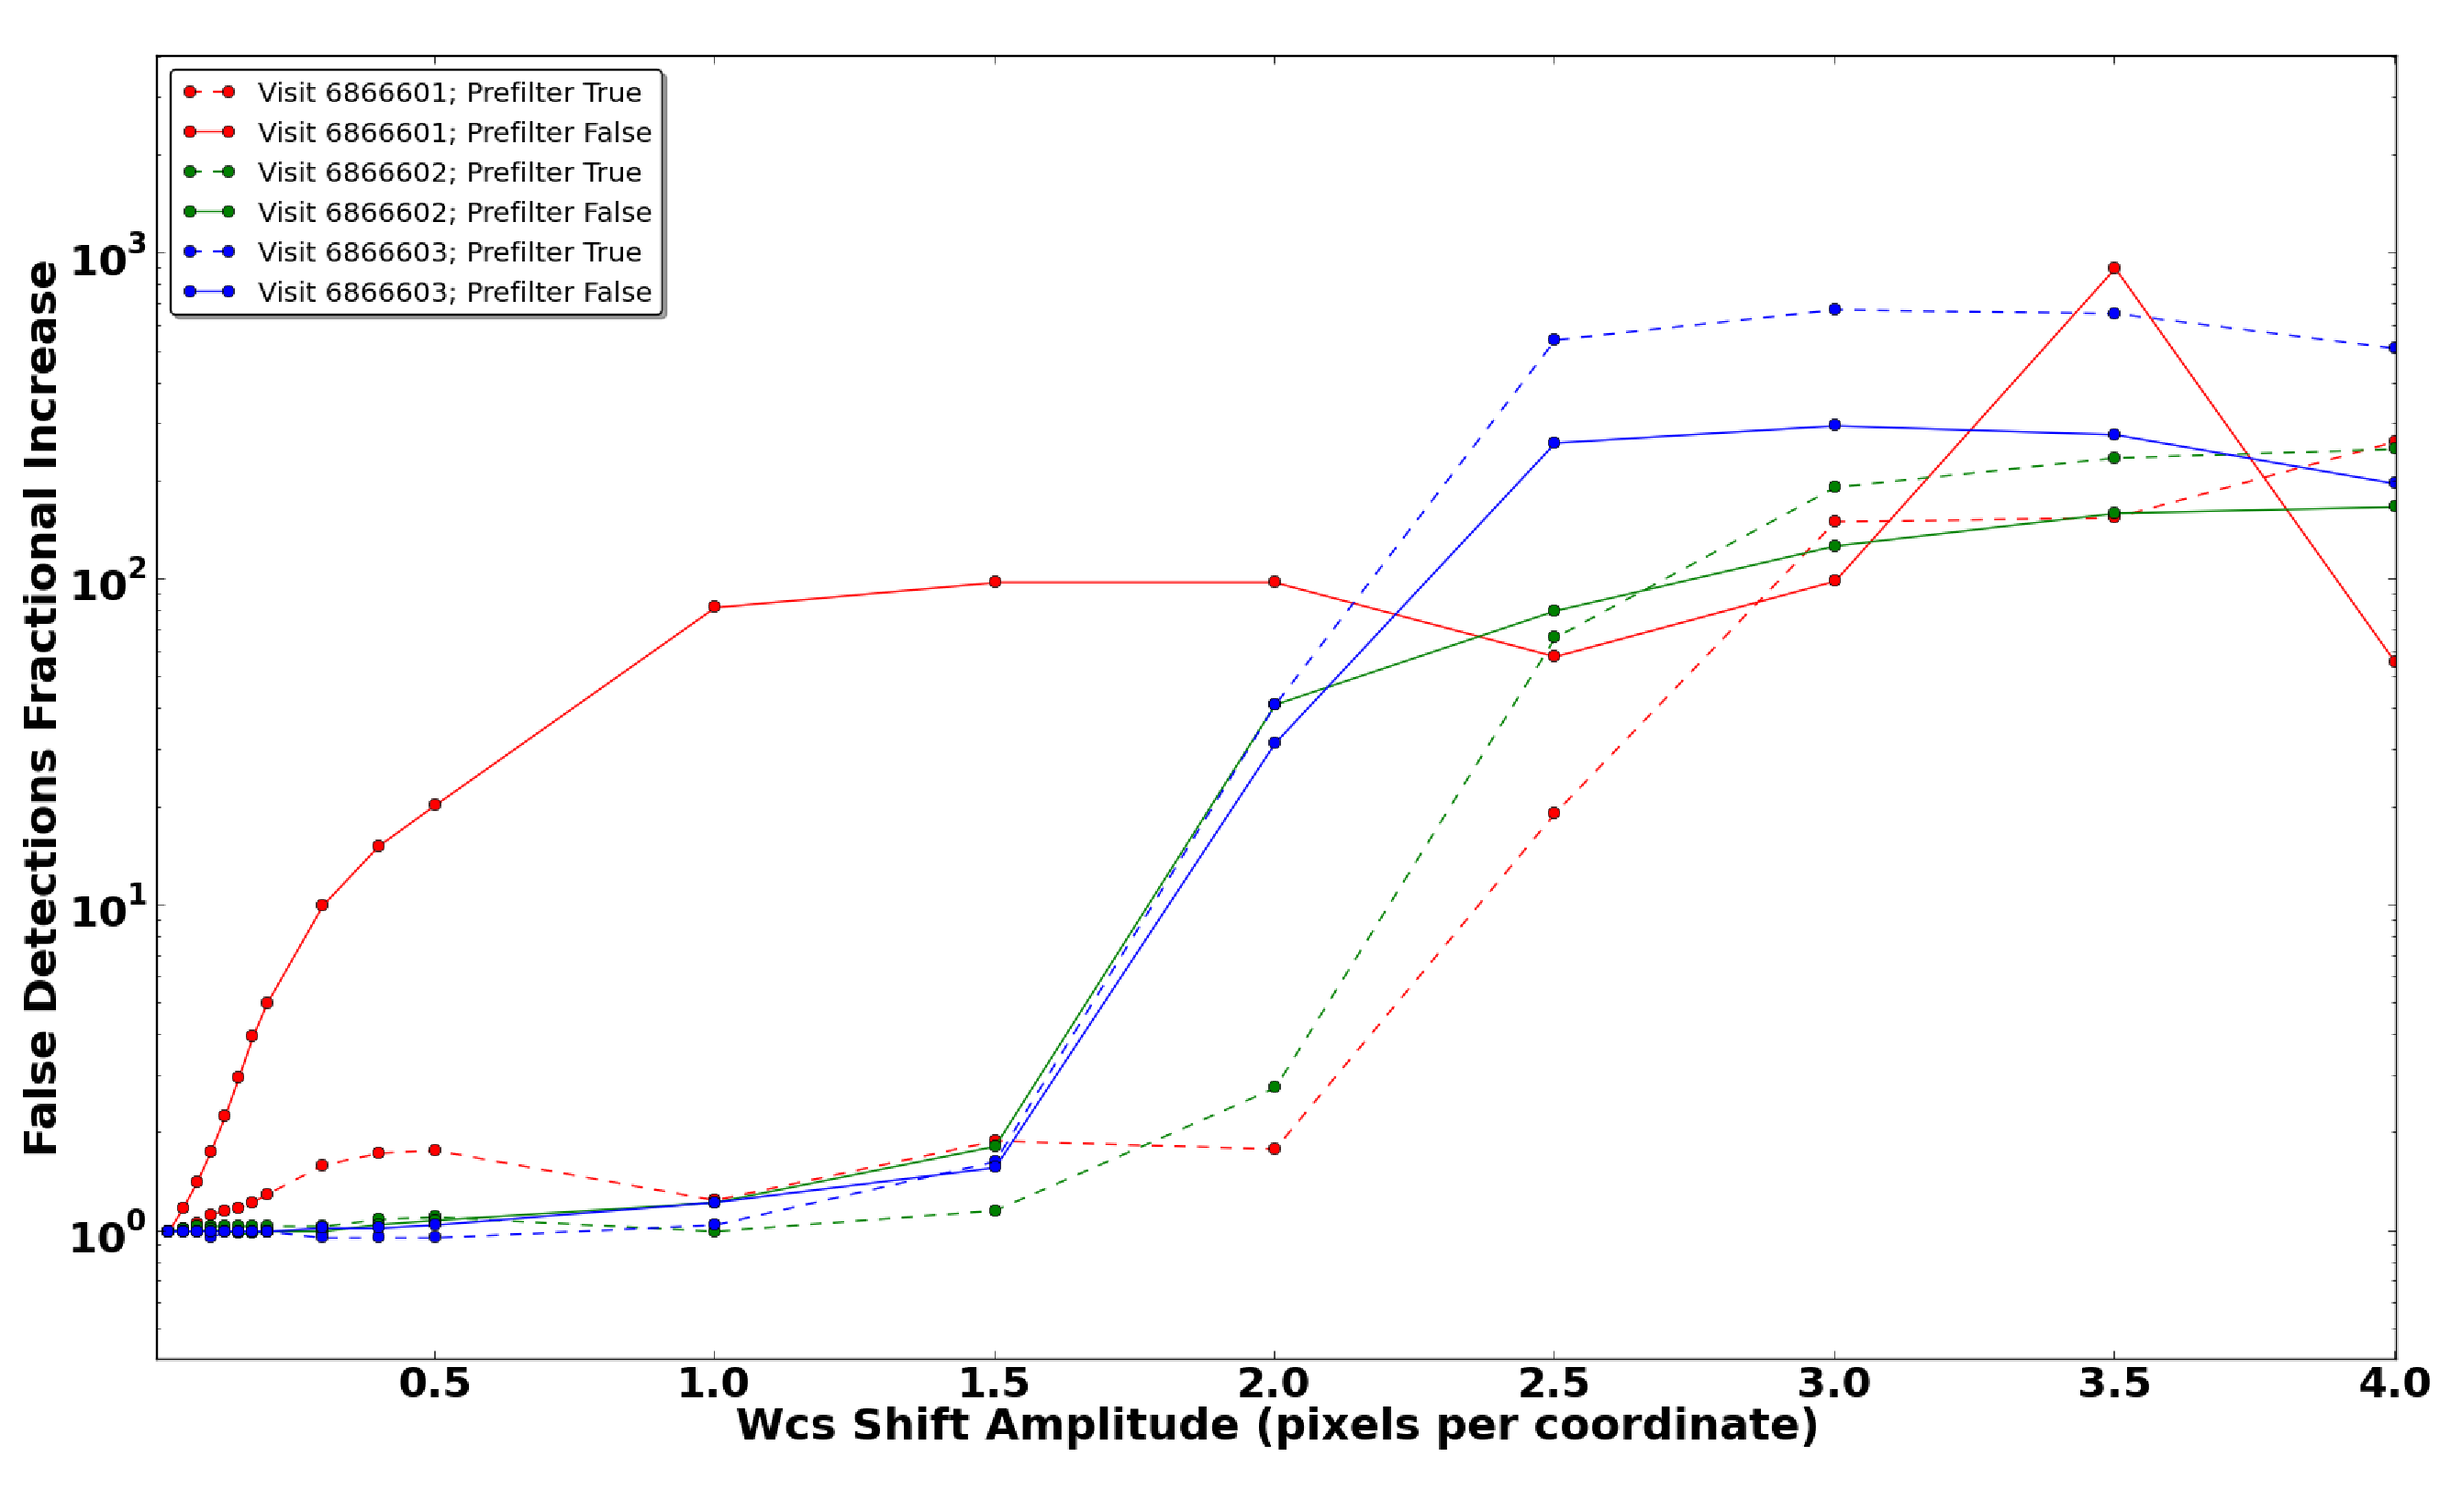
\includegraphics[width=1.0\textwidth]{figures/wcs_shift.eps}} \\
\caption{Fractional increase in false detections as a function of bulk
  astrometric offsets added to the coordinates of sources before
  image-to-image registration.  The {\it red}, {\it green}, and {\it
    blue} lines correspond to visits v6866601, v6866602, and v6866603
  respectively, while the {\it dashed} and {\it solid} lines
  correspond to prefiltering and postfiltering, respectively.}
\label{wcsshift}
\end{figure}

\begin{figure}
\centering{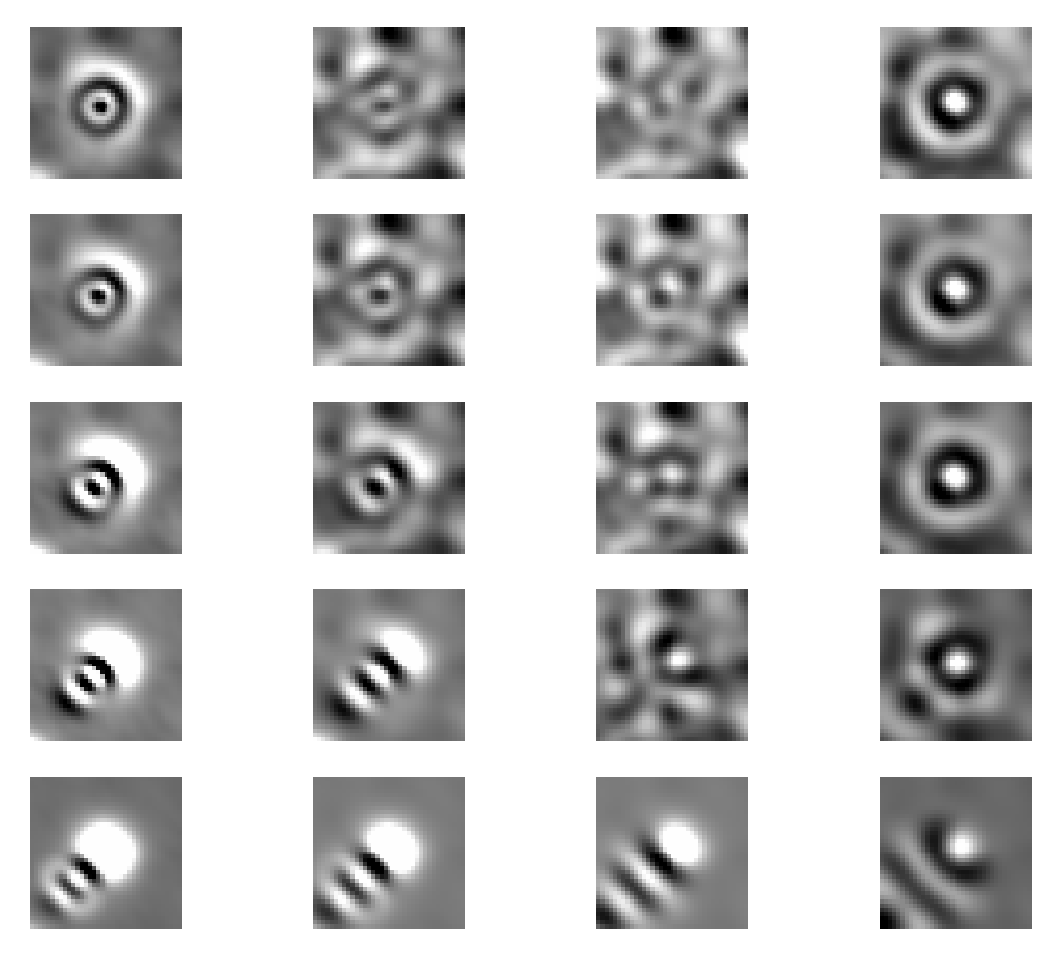
\includegraphics[width=0.8\textwidth]{figures/shift.eps}} \\
\caption{Figure illustrating the ability of the kernel basis to
  compensate, locally, for the effects of misregistration.  Each
  element of the grid shows a single {\tt KernelCandidate} local
  difference image (visit=6866603, doPreFilter=True).  Columns
  indicate the Gaussian sigma of the basis, which is designed to have
  one Gaussian with the prescribed width, modified to fourth order.
  Rows indicate the amplitude of the astrometric offset that was
  introduced into the Source positions before image-to-image
  registration.  In the {\it top} row, we see that even with a small
  astrometric offset, the sigma=2 basis is unable to produce a quality
  subtraction, because the width is inappropriate for matching the two
  input PSFs (the theoretical Gaussian matching sigma here is 3.4 pixels).  At
  sigma=4 the basis is able to produce a quality subtraction, and by
  sigma=5 the basis is too large to match the PSFs.  In {\it row 4},
  we show that even for an astrometric offset of 4 pixels (0.8''), the
  sigma=4 basis can produce a reasonable difference image without
  structured residuals.  However, by {\it row 5}, with an offset of 6
  pixels, none of the Gaussians provide a successful local difference
  image.  The ability of the basis to compensate for bulk astrometric
  offsets is a function of the kernel width, and the kernel width is
  itself a function of the two input PSF FWHMs.  Thus there is a
  complicated dependence of the ability of the kernel to shift the
  centroids of stars.  Roughly, in our implementation, the basis may
  compensate for local astrometric residuals at a scale up to $\beta
  \times \sqrt{\sigma_S^2 - \sigma_T^2}$, which is the width of the
  largest Gaussian in our bases.}
\label{kernel_offsets}
\end{figure}


\begin{figure}%
\captionsetup[subfloat]{labelformat=empty}
\centering
\subfloat[]{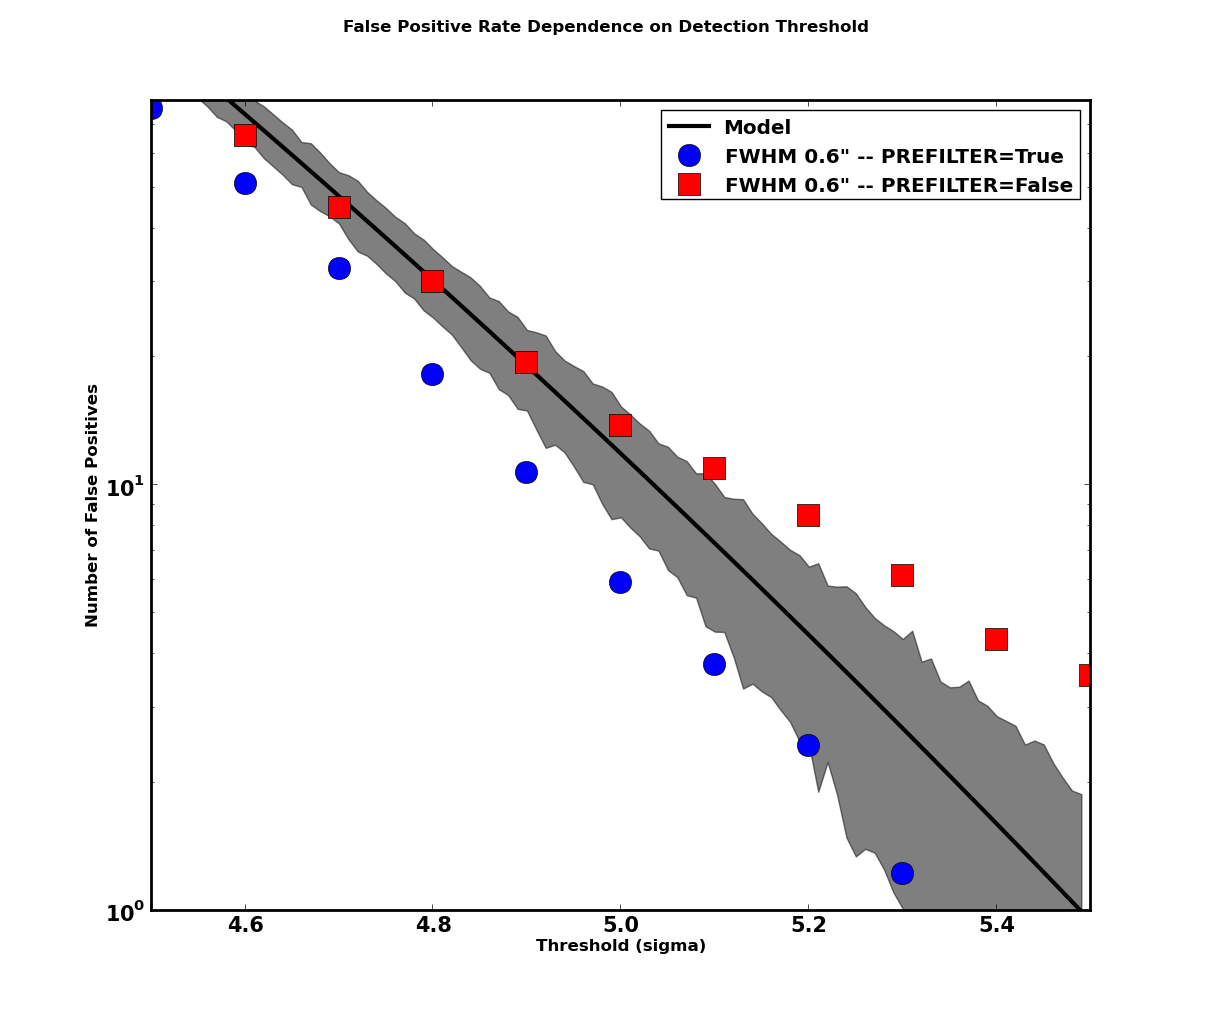
\includegraphics[width=0.3\textwidth]{figures/fp_v_thresh_01_nocorr.eps}}
\subfloat[]{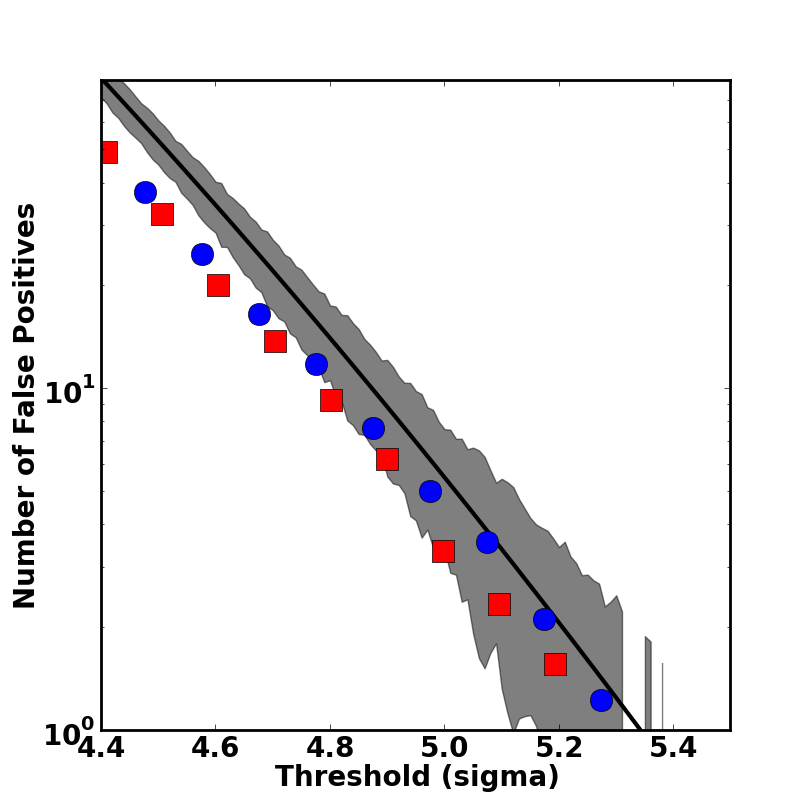
\includegraphics[width=0.3\textwidth]{figures/fp_v_thresh_02_nocorr.eps}}
\subfloat[]{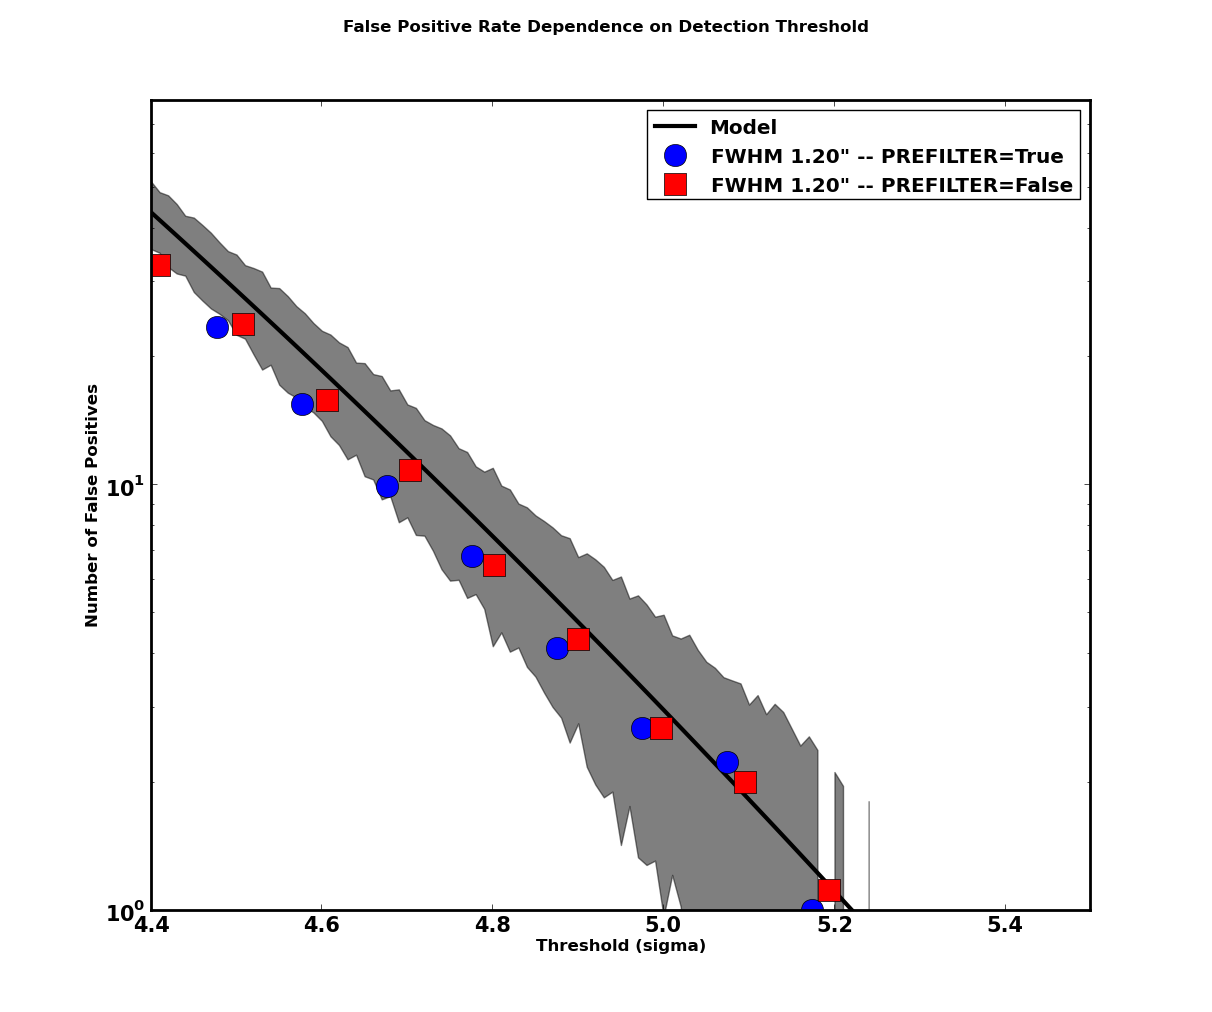
\includegraphics[width=0.3\textwidth]{figures/fp_v_thresh_03_nocorr.eps}}\\
\subfloat[]{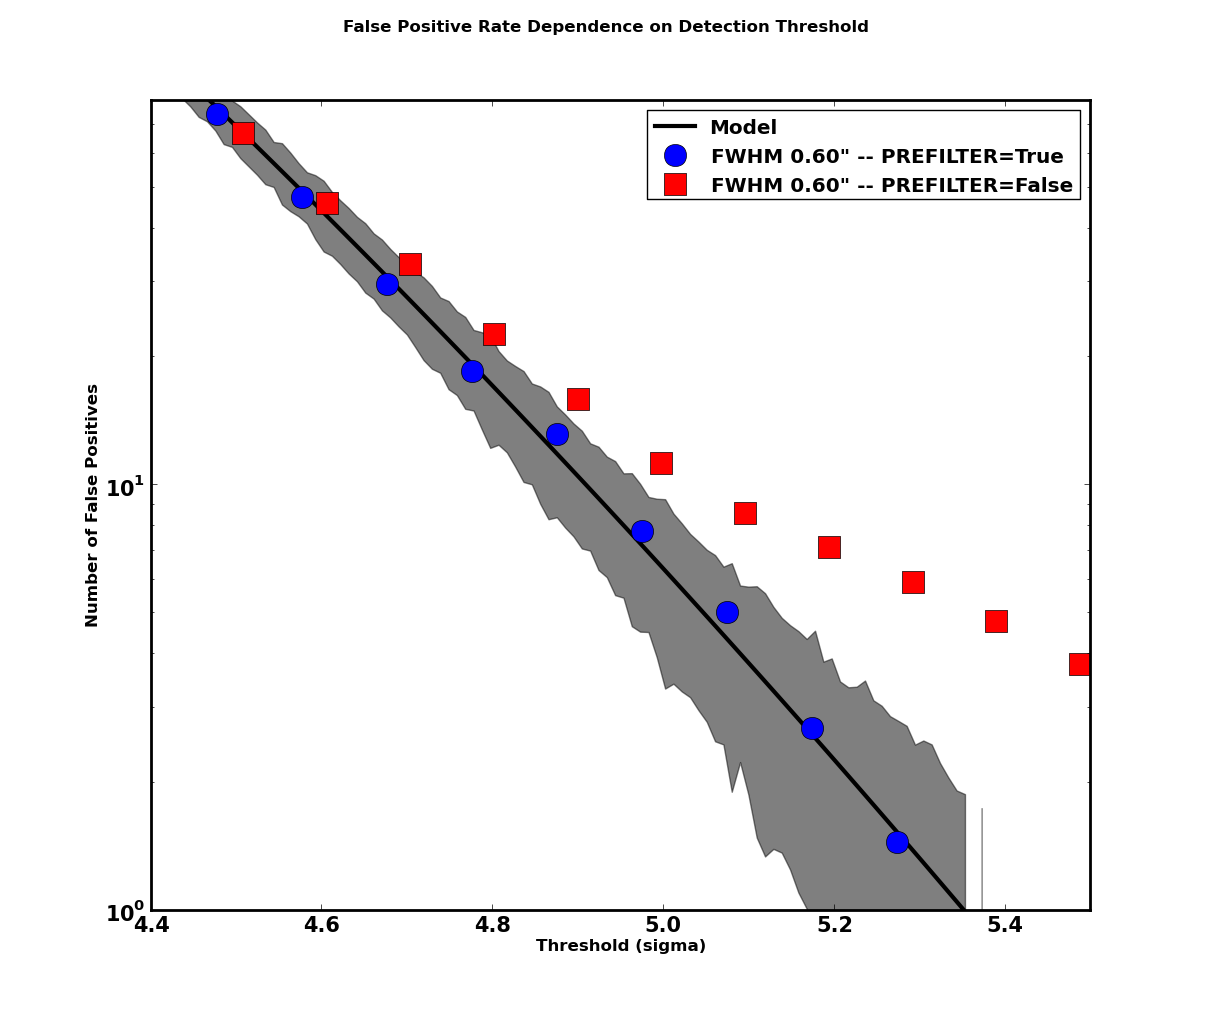
\includegraphics[width=0.3\textwidth]{figures/fp_v_thresh_01_corr.eps}}%
\subfloat[]{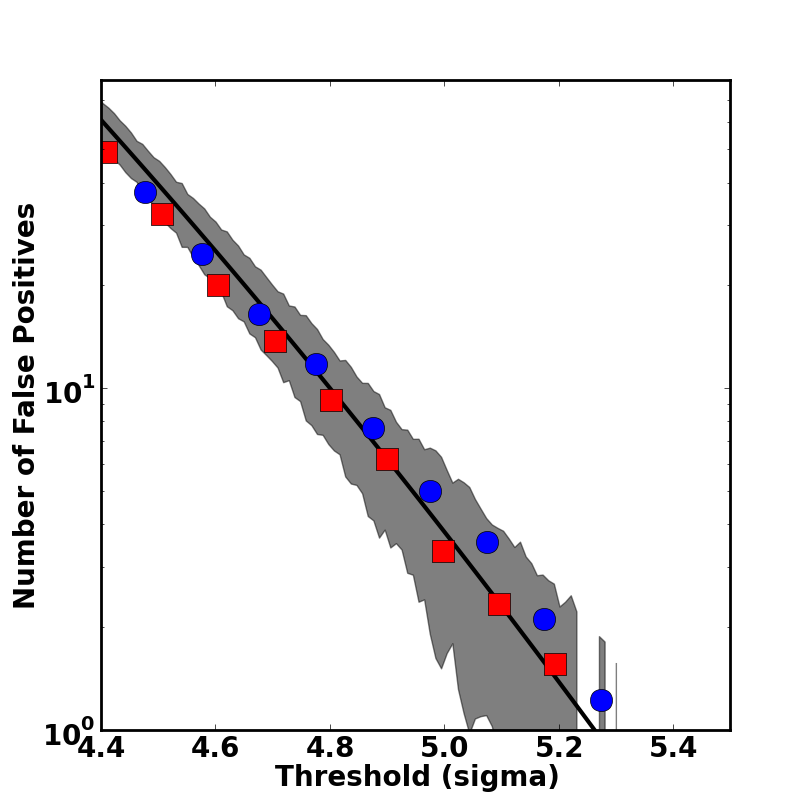
\includegraphics[width=0.3\textwidth]{figures/fp_v_thresh_02_corr.eps}}%
\subfloat[]{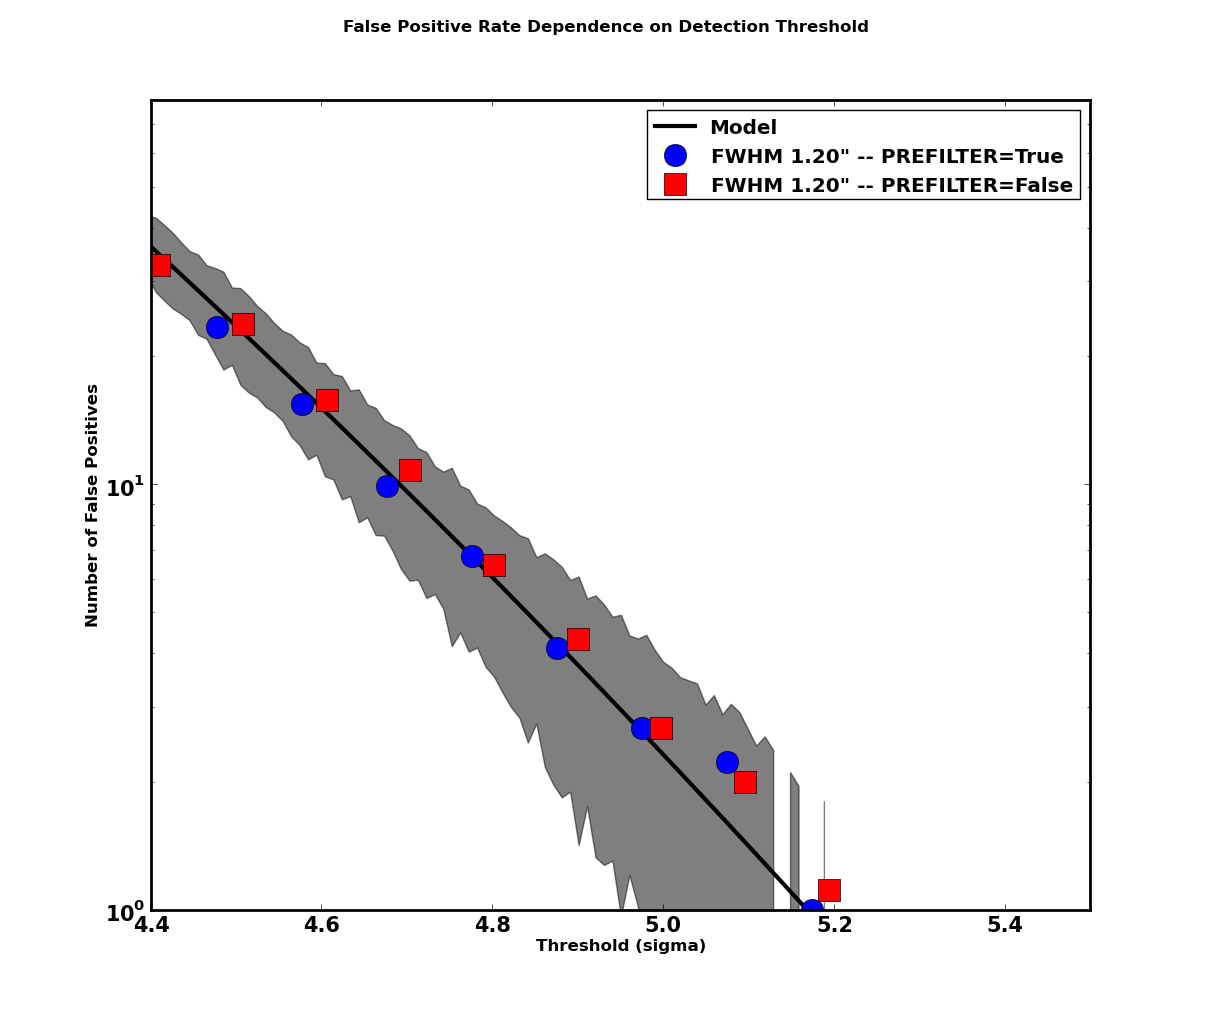
\includegraphics[width=0.3\textwidth]{figures/fp_v_thresh_03_corr.eps}}%
\caption{}
\label{fig-fp_v_thresh}
\end{figure}


\begin{figure}
\begin{center}
\centering{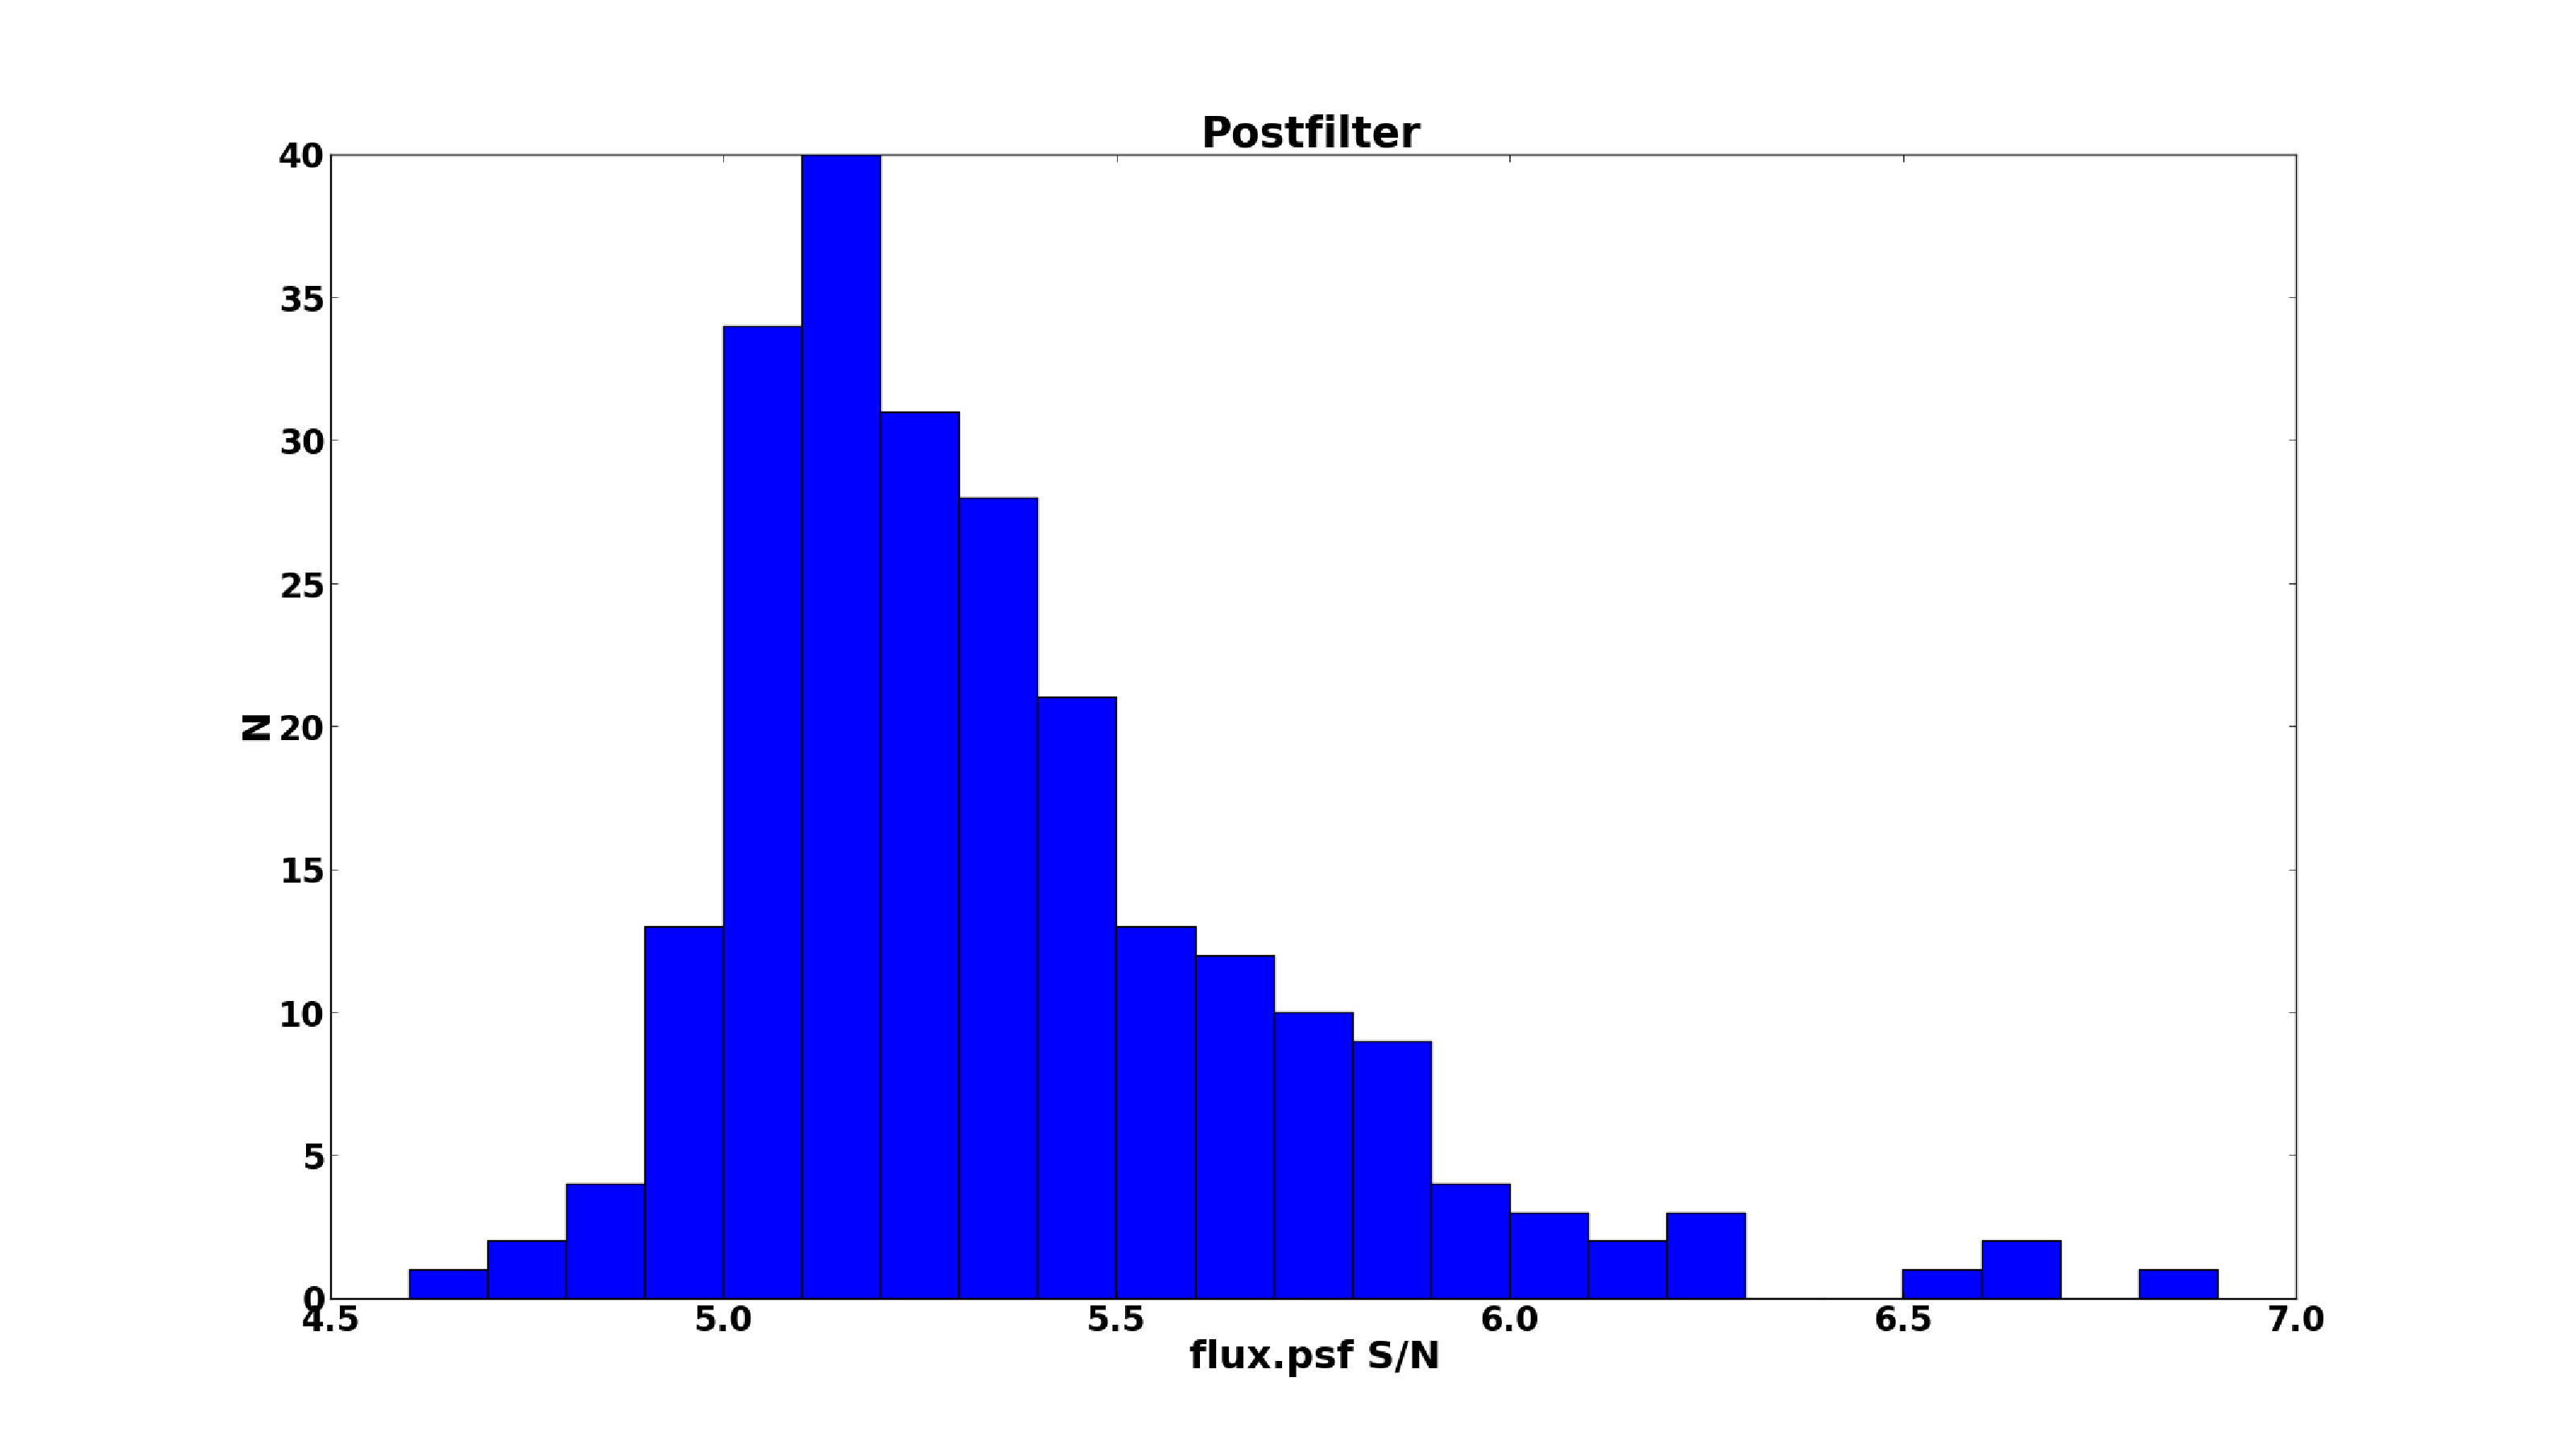
\includegraphics[width=0.9\textwidth]{figures/fluxpost.eps}} \\
\centering{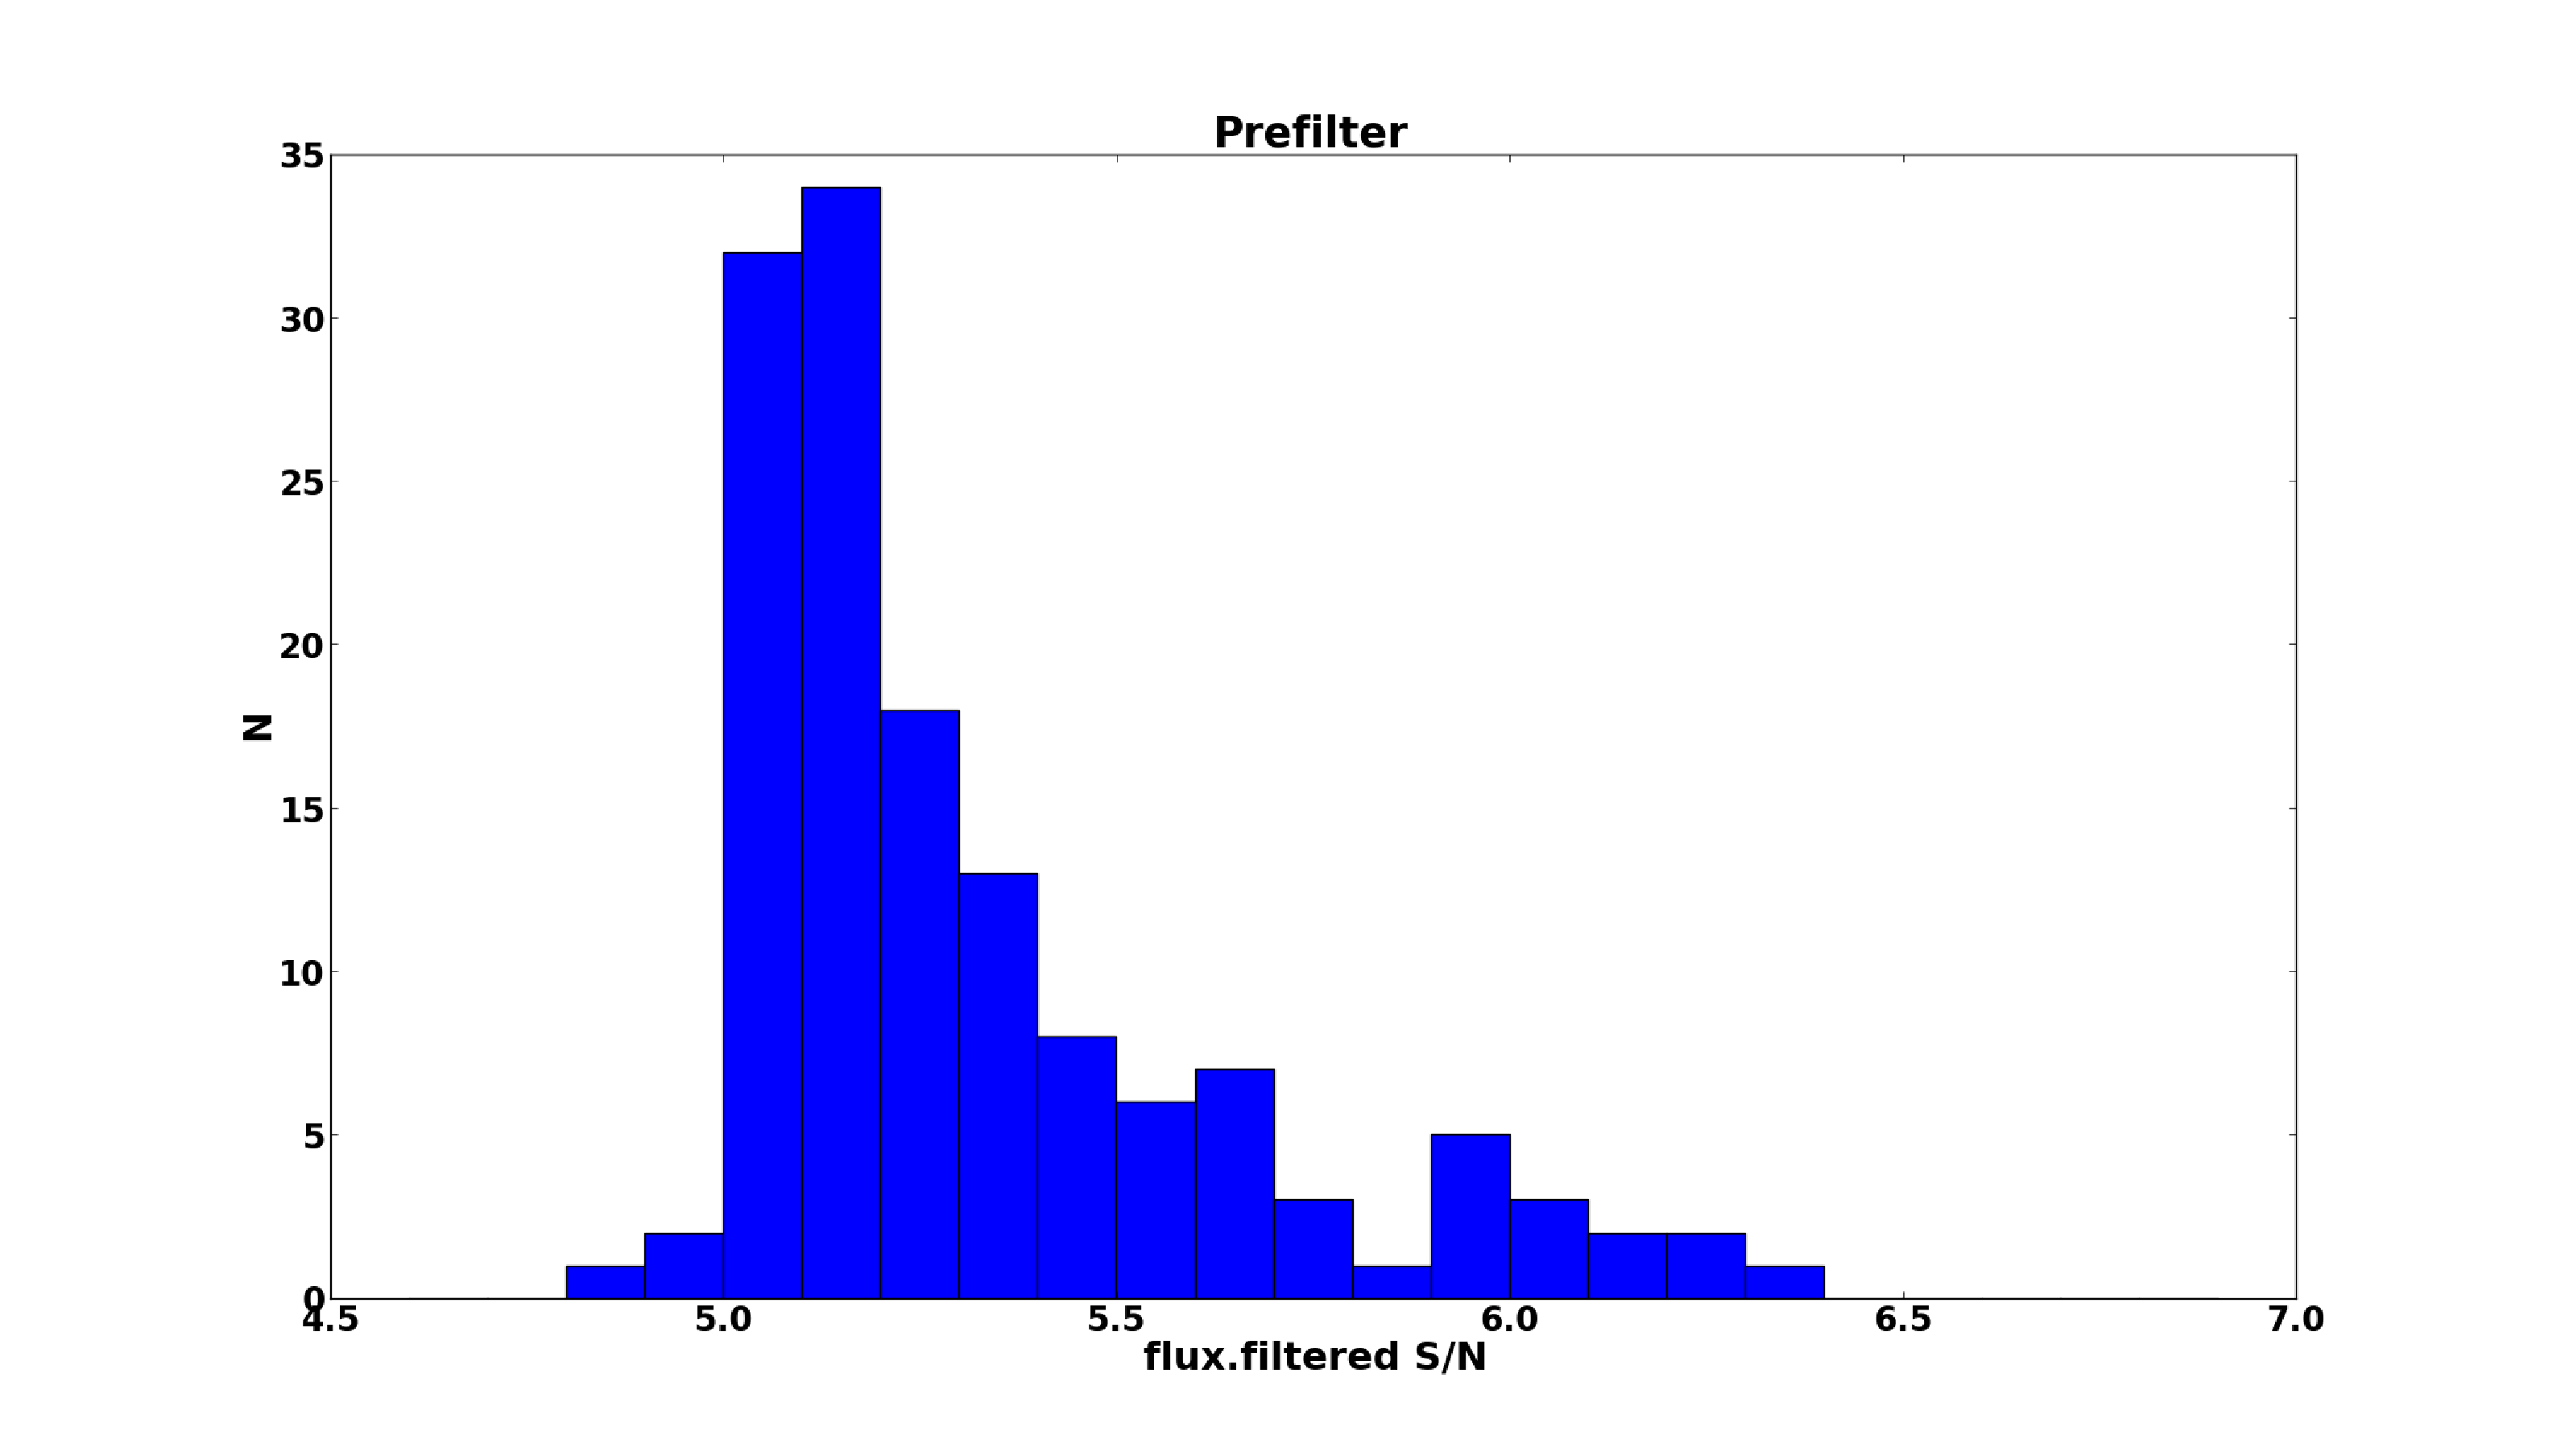
\includegraphics[width=0.9\textwidth]{figures/fluxpre.eps}} \\
\end{center}
\caption{Histograms of measured $|$ signal--to--noise $|$
  for sources detected at 5--sigma in the best postfiltered ({\it
    top}) and prefiltered ({\it bottom}) data.  In postfiltering, we
  use the PSF flux, while in prefiltering we use the filtered flux
  measurement.  }
\label{fluxerr}
\end{figure}

\begin{figure}
\centering{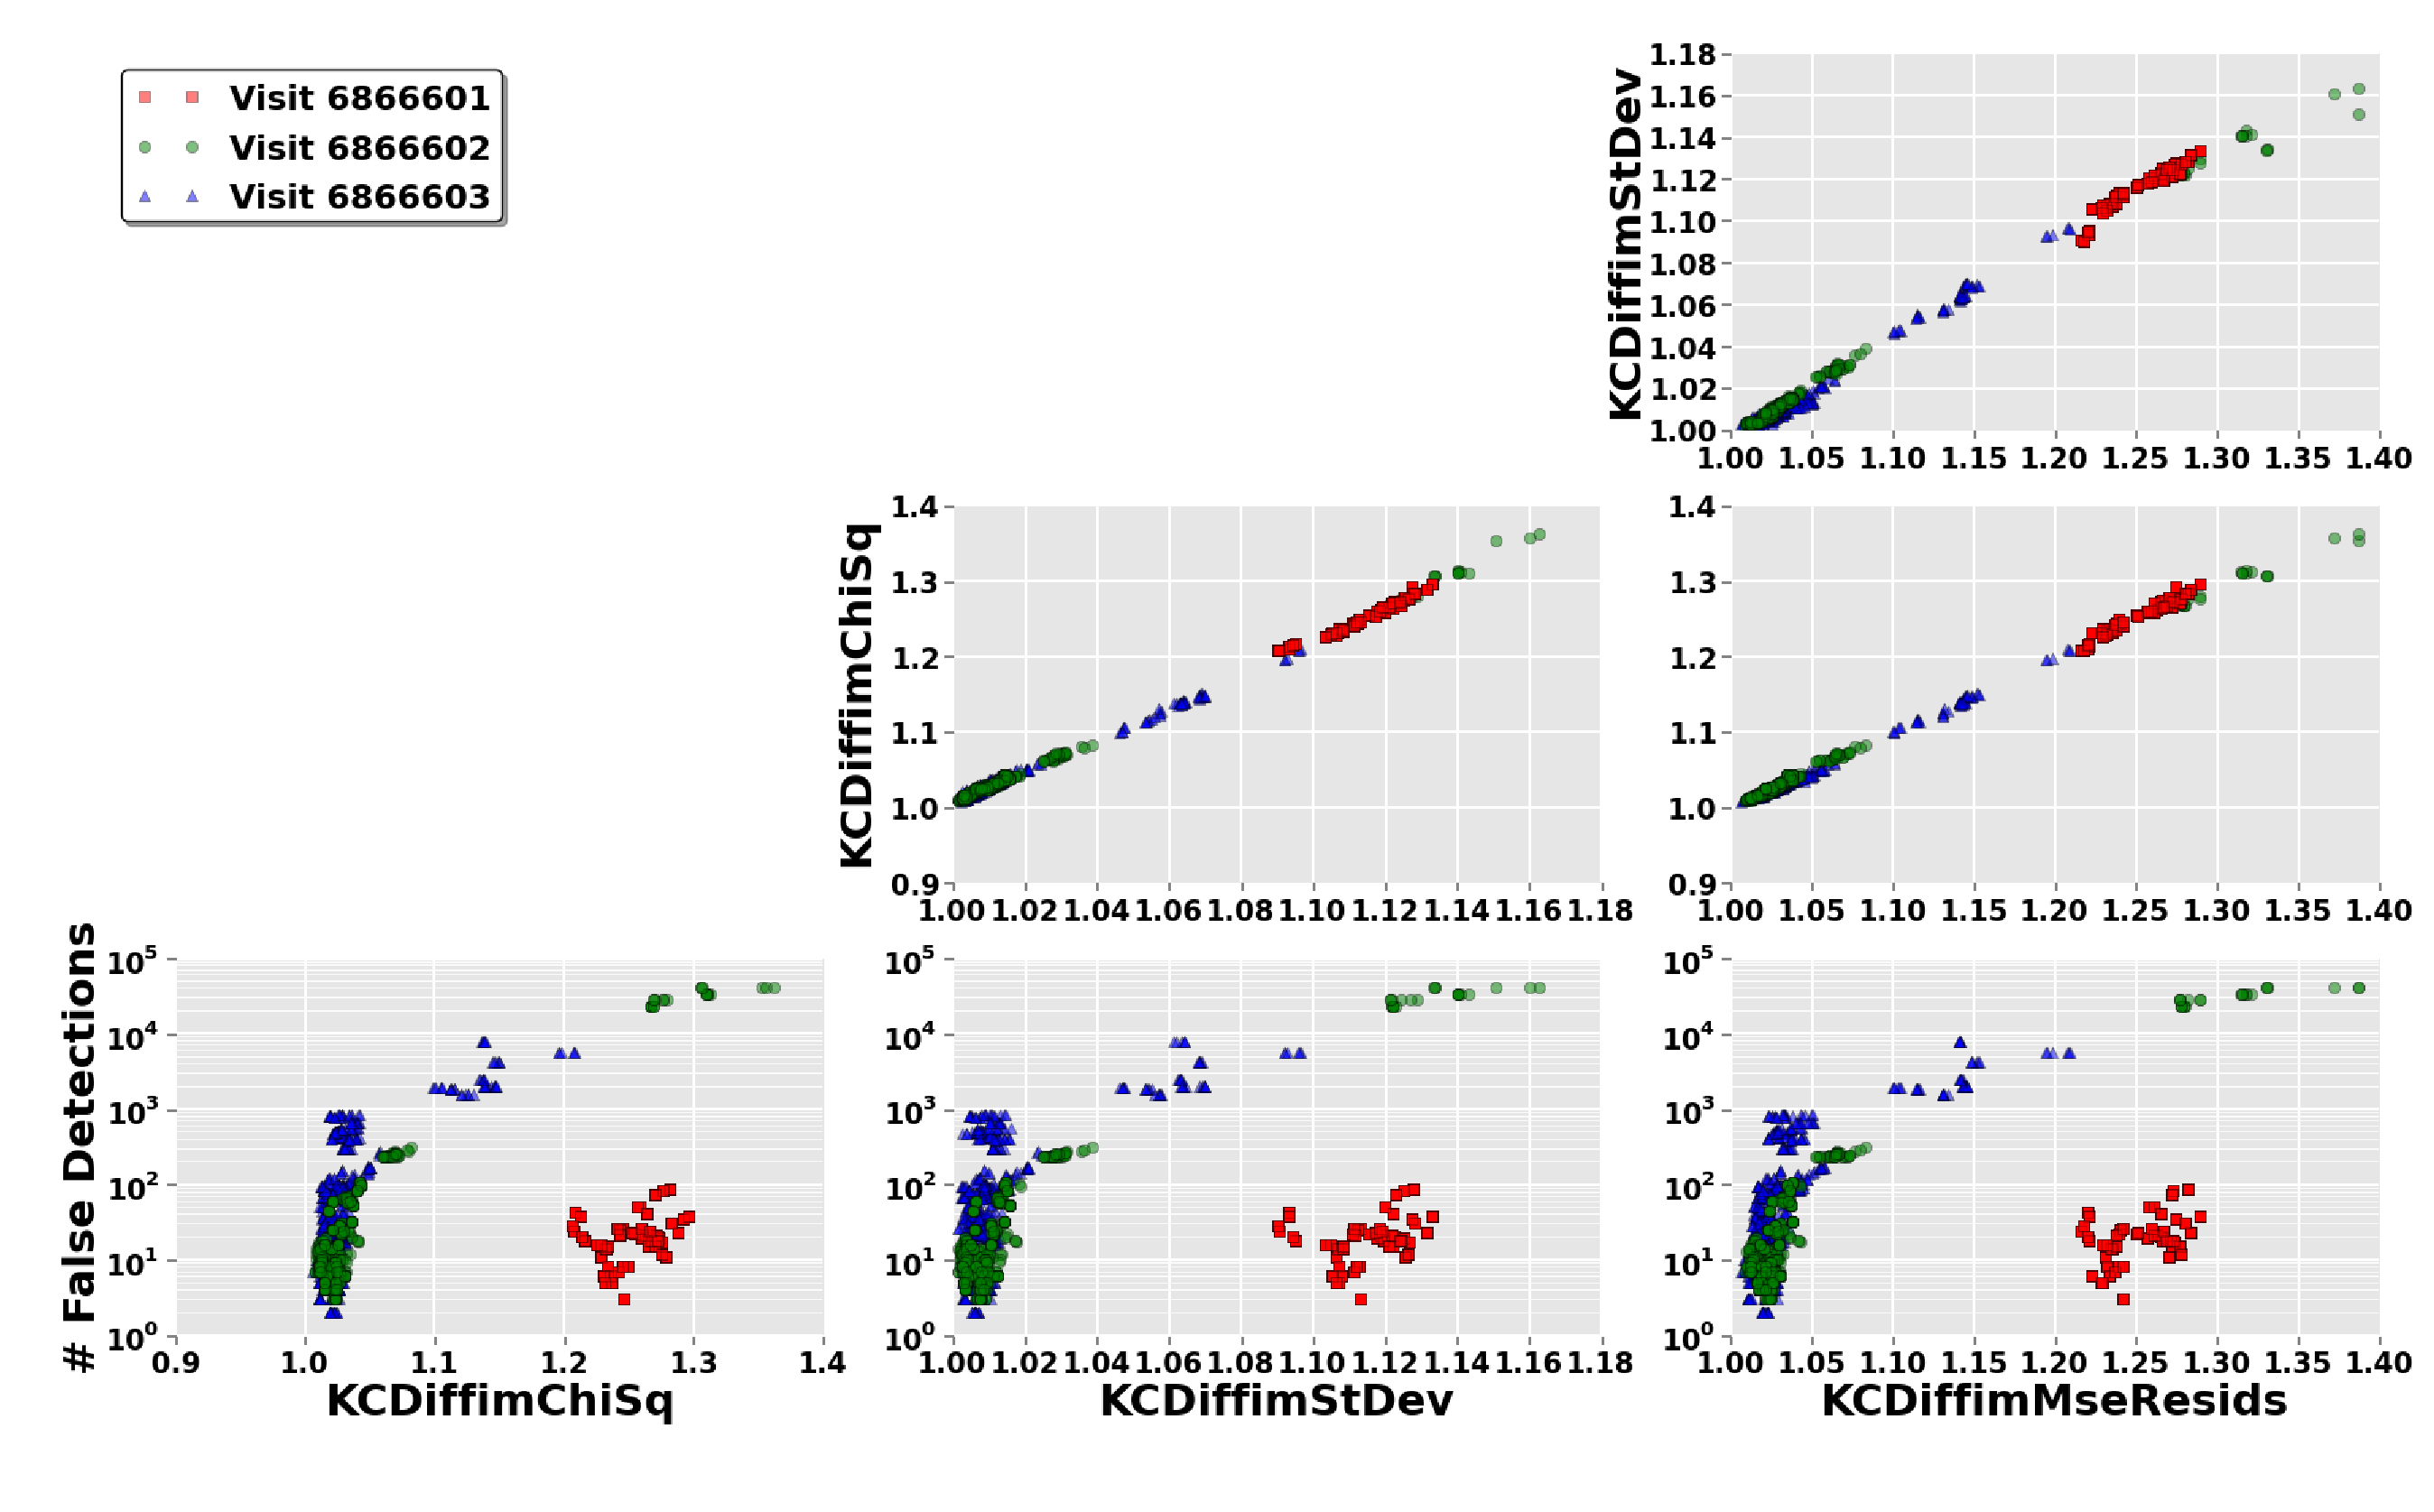
\includegraphics[width=0.9\textwidth]{figures/corrA.eps}} \\
\caption{Correlation of the statistics calculated on the control
  sample {\tt KernelCandidates} during the model fitting with the
  number of false positives per sensor coming from
  detection and measurement, for the {\bf postfiltering} pipeline.
  Results for visit v6866601 are shown as {\it red squares}, for
  v6866602 as {\it green circles}, and for v6866603 {\it blue
    triangles}.  Three of the statistics, described in
  Section~\ref{sec-stats}, are presented.  They clearly correlate with
  each other.  For the deconvolution visit v6866601, the statistics
  are very poor even for the ``best'' solutions.  
}
\label{corrpost}
\end{figure}

\begin{figure}
\centering{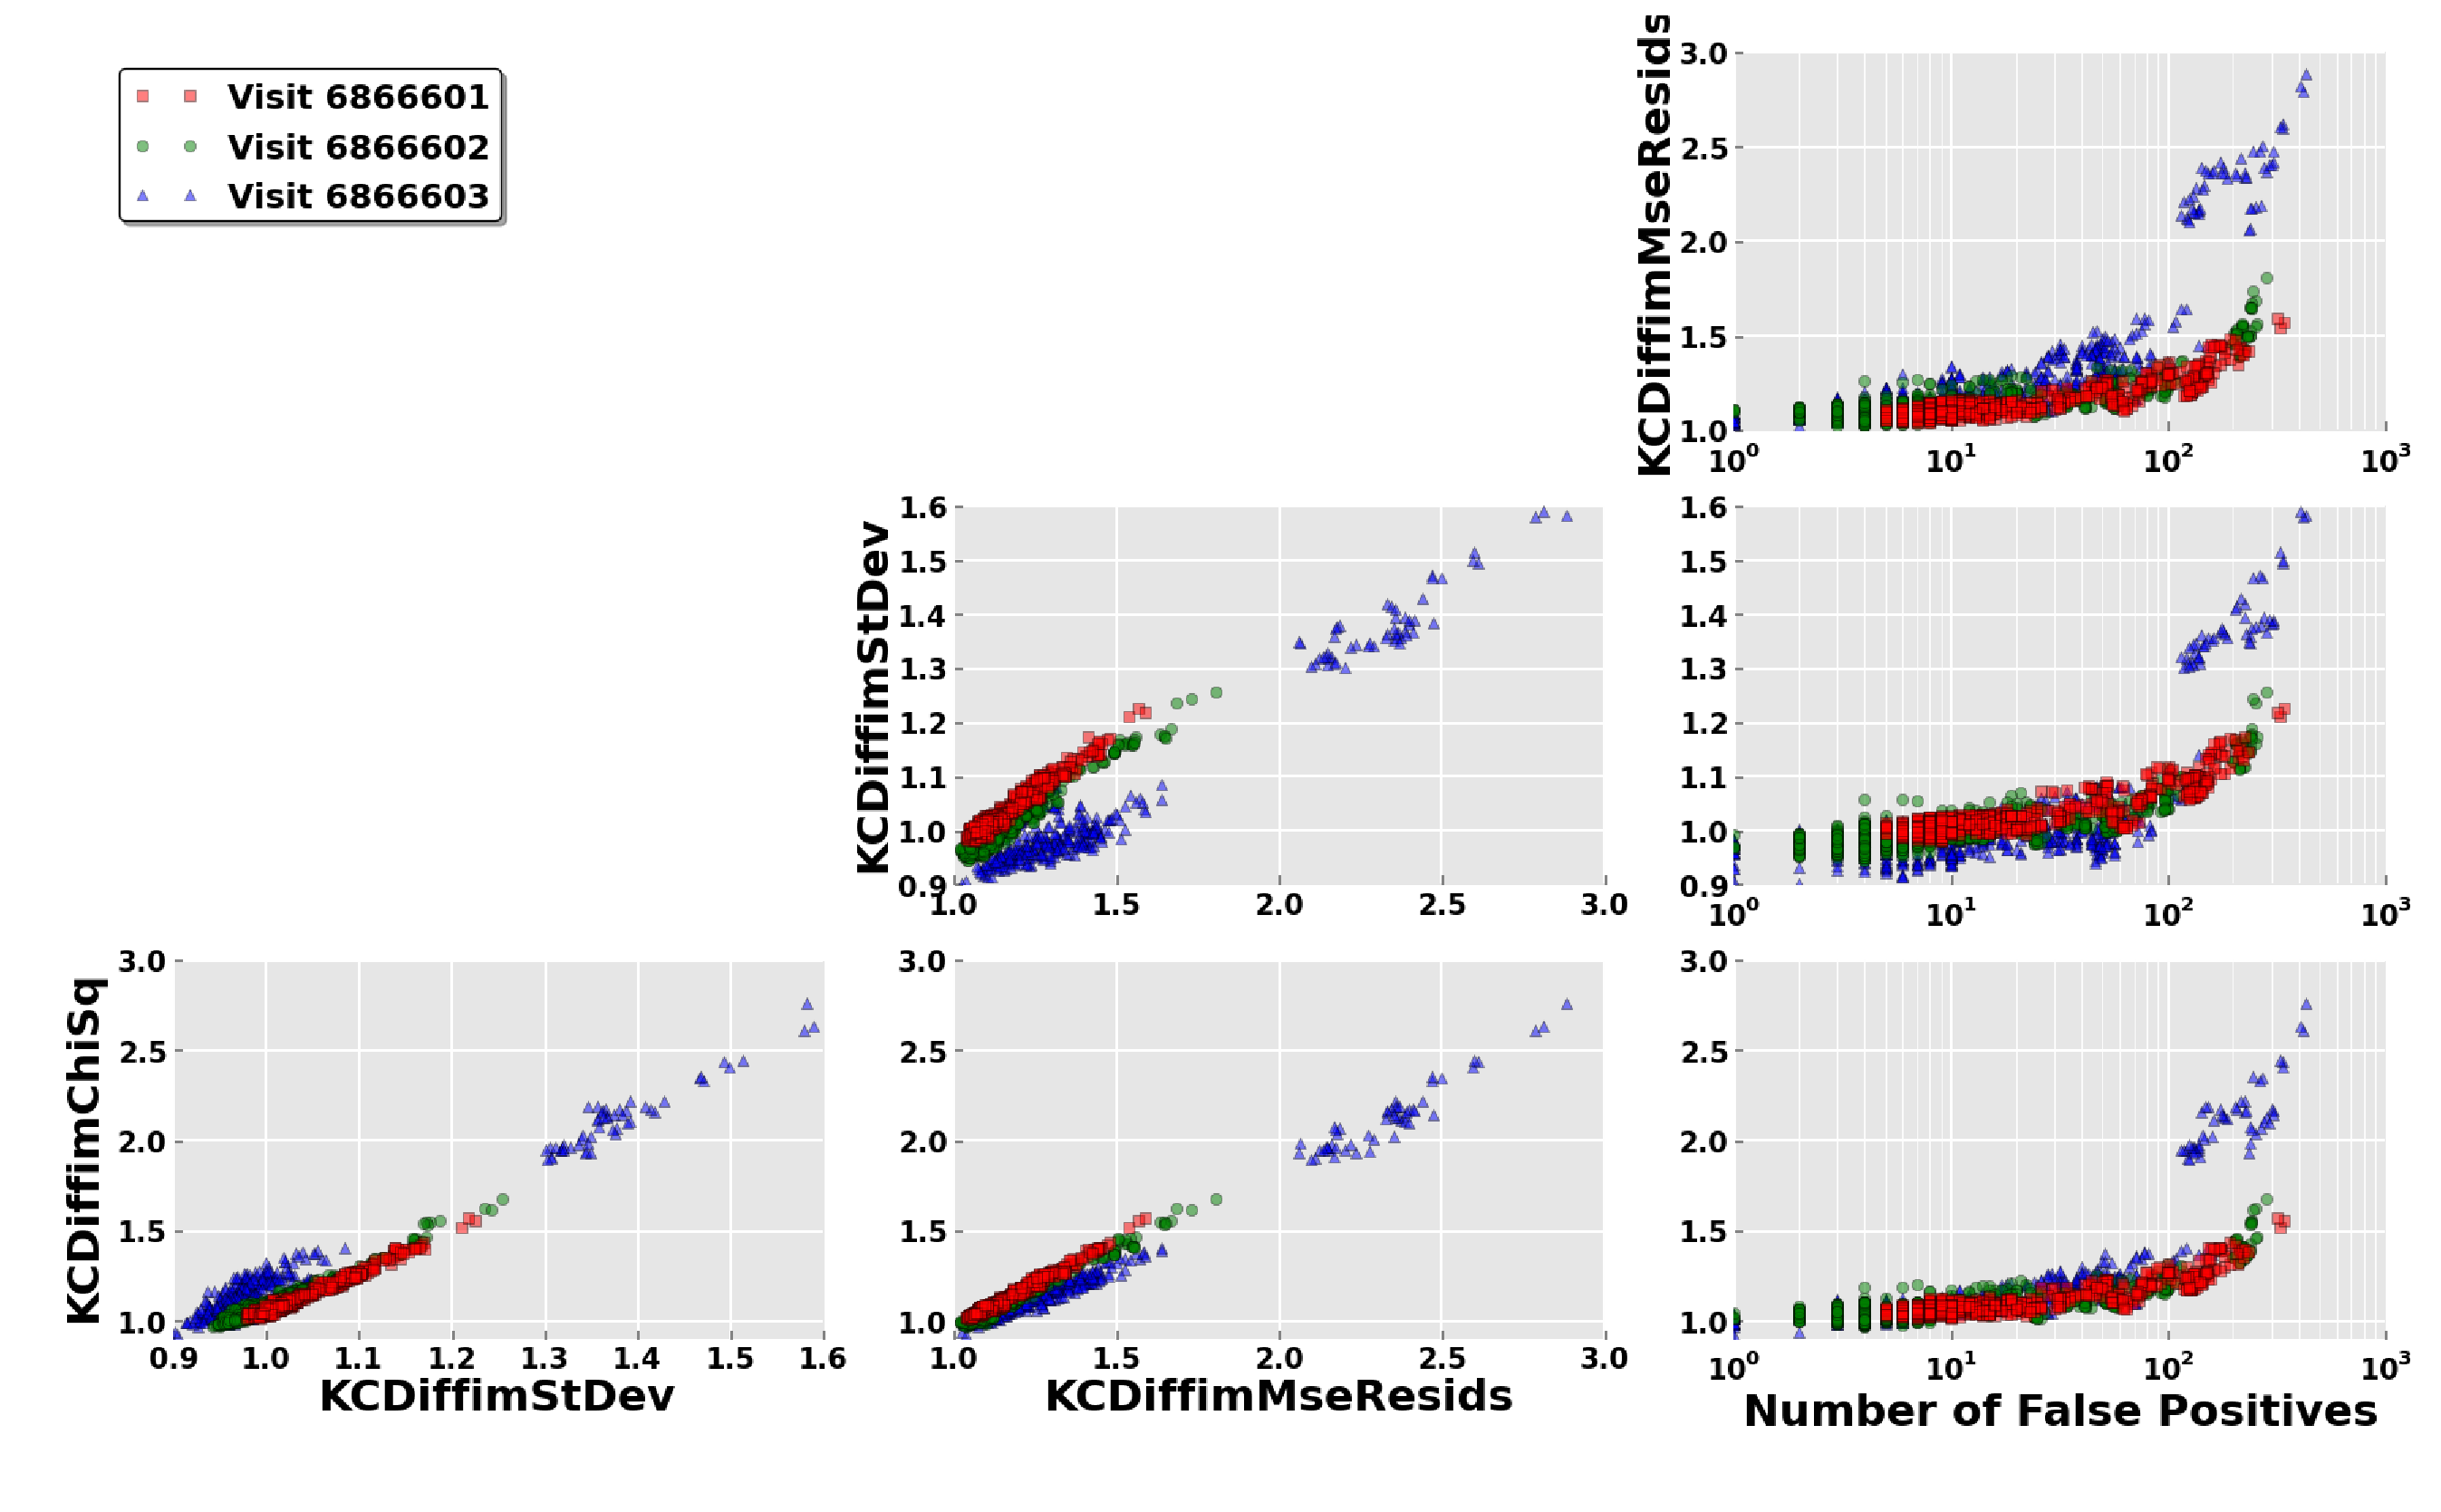
\includegraphics[width=0.9\textwidth]{figures/corrB.eps}} \\
\caption{Correlation of the statistics calculated on the control
  sample {\tt KernelCandidates} during the model fitting with the
  number of false positives per sensor coming from detection and
  measurement, for the {\bf prefiltering} pipeline.  Results for visit
  v6866601 are shown as {\it red squares}, for v6866602 as {\it green
    circles}, and for v6866603 {\it blue triangles}.  Three of the
  statistics, described in Section~\ref{sec-stats}, are presented.
  They clearly correlate with each other, and also tend to correlate
  with the number of false detections (bottom row).}
\label{corrpre}
\end{figure}

\clearpage 
\begin{appendices}
\section{Phosim Configuration for Production Data \label{sec-phosim}}
\begin{verbatim}
zenith_v 23.0
qevariation 0.0
backbeta 4
raydensity 0.0
airglowvariation 0
cleartracking
clearperturbations
clearclouds
saturation 0
blooming 0
diffractionmode 0
centroidfile 1
\end{verbatim}

\section{Phosim Data for Extended Analysis \label{sec-phosimextend}}

Images for the extended analysis contain stars and galaxies, at
densities appropriate for high Galactic latitudes, with a range of
spectral energy distributions, but with no asteroids, no variability,
no cosmic rays, and no proper motions or parallax.  Images simulated
from these catalogs were generated using the input parameters
described above, with the following exceptions.

Visit 11111111 was generated for the $i$-band:
\begin{itemize}
\item Visit 1111111100: A pair of 300s exposure template images with
  an atmospheric seeing value of 0.88 arcsec.
\item Visit 1111111101: A pair of 15s exposure exposures with 0.6
arcsec atmospheric seeing at zenith.
\item Visit 1111111102: A pair of 15s exposure exposures with 0.88
arcsec atmospheric seeing at zenith.
\item Visit 1111111103: A pair of 15s exposure exposures with 1.2
arcsec atmospheric seeing at an altitude of 45 degrees.
\item Visit 1111111104: A pair of 15s exposure exposures with 0.6
arcsec atmospheric seeing at an altitude of 45 degrees.
\item Visit 1111111105: A pair of 15s exposure exposures with 0.88
arcsec atmospheric seeing at an altitude of 45 degrees.
\item Visit 1111111106: A pair of 15s exposure exposures with 1.2
arcsec atmospheric seeing at an altitude of 45 degrees.
\end{itemize}

Visit 22222222 was generated for the $g$-band:
 \begin{itemize}
\item Visit 2222222200: A pair of 300s exposure template images with
  an atmospheric seeing value is 0.88 arcsec.
\item Visit 2222222201: A pair of 15s exposure exposures with 0.6
arcsec atmospheric seeing at zenith.
\item Visit 2222222202: A pair of 15s exposure exposures with 0.88
arcsec atmospheric seeing at zenith.
\item Visit 2222222203: A pair of 15s exposure exposures with 1.2
arcsec atmospheric seeing at an altitude of 45 degrees.
\item Visit 2222222204: A pair of 15s exposure exposures with 0.6
arcsec atmospheric seeing at an altitude of 45 degrees.
\item Visit 2222222205: A pair of 15s exposure exposures with 0.88
arcsec atmospheric seeing at an altitude of 45 degrees.
\item Visit 2222222206: A pair of 15s exposure exposures with 1.2
arcsec atmospheric seeing at an altitude of 45 degrees.
\end{itemize}

\end{appendices}

\end{document}
